% Generated by Sphinx.
\def\sphinxdocclass{report}
\documentclass[a4paper,11pt,english]{sphinxmanual}
\usepackage[utf8]{inputenc}
\DeclareUnicodeCharacter{00A0}{\nobreakspace}
\usepackage{cmap}
\usepackage[T1]{fontenc}
\usepackage{babel}
\usepackage{times}
\usepackage[Bjarne]{fncychap}
\usepackage{longtable}
\usepackage{sphinx}
\usepackage{multirow}

\usepackage{mathpazo}
\usepackage{courier}
\usepackage[scaled=0.9]{berasans}
\let\oldprintindex\printindex
\def\printindex{\raggedright\oldprintindex}


\title{JuliaBase}
\date{February 13, 2015}
\release{1.0c}
\author{Torsten Bronger}
\newcommand{\sphinxlogo}{
\includegraphics{juliabase_logo.pdf}\par}
\renewcommand{\releasename}{Release}
\makeindex

\makeatletter
\def\PYG@reset{\let\PYG@it=\relax \let\PYG@bf=\relax%
    \let\PYG@ul=\relax \let\PYG@tc=\relax%
    \let\PYG@bc=\relax \let\PYG@ff=\relax}
\def\PYG@tok#1{\csname PYG@tok@#1\endcsname}
\def\PYG@toks#1+{\ifx\relax#1\empty\else%
    \PYG@tok{#1}\expandafter\PYG@toks\fi}
\def\PYG@do#1{\PYG@bc{\PYG@tc{\PYG@ul{%
    \PYG@it{\PYG@bf{\PYG@ff{#1}}}}}}}
\def\PYG#1#2{\PYG@reset\PYG@toks#1+\relax+\PYG@do{#2}}

\expandafter\def\csname PYG@tok@gd\endcsname{\def\PYG@tc##1{\textcolor[rgb]{0.63,0.00,0.00}{##1}}}
\expandafter\def\csname PYG@tok@gu\endcsname{\let\PYG@bf=\textbf\def\PYG@tc##1{\textcolor[rgb]{0.50,0.00,0.50}{##1}}}
\expandafter\def\csname PYG@tok@gt\endcsname{\def\PYG@tc##1{\textcolor[rgb]{0.00,0.27,0.87}{##1}}}
\expandafter\def\csname PYG@tok@gs\endcsname{\let\PYG@bf=\textbf}
\expandafter\def\csname PYG@tok@gr\endcsname{\def\PYG@tc##1{\textcolor[rgb]{1.00,0.00,0.00}{##1}}}
\expandafter\def\csname PYG@tok@cm\endcsname{\let\PYG@it=\textit\def\PYG@tc##1{\textcolor[rgb]{0.25,0.50,0.56}{##1}}}
\expandafter\def\csname PYG@tok@vg\endcsname{\def\PYG@tc##1{\textcolor[rgb]{0.73,0.38,0.84}{##1}}}
\expandafter\def\csname PYG@tok@m\endcsname{\def\PYG@tc##1{\textcolor[rgb]{0.13,0.50,0.31}{##1}}}
\expandafter\def\csname PYG@tok@mh\endcsname{\def\PYG@tc##1{\textcolor[rgb]{0.13,0.50,0.31}{##1}}}
\expandafter\def\csname PYG@tok@cs\endcsname{\def\PYG@tc##1{\textcolor[rgb]{0.25,0.50,0.56}{##1}}\def\PYG@bc##1{\setlength{\fboxsep}{0pt}\colorbox[rgb]{1.00,0.94,0.94}{\strut ##1}}}
\expandafter\def\csname PYG@tok@ge\endcsname{\let\PYG@it=\textit}
\expandafter\def\csname PYG@tok@vc\endcsname{\def\PYG@tc##1{\textcolor[rgb]{0.73,0.38,0.84}{##1}}}
\expandafter\def\csname PYG@tok@il\endcsname{\def\PYG@tc##1{\textcolor[rgb]{0.13,0.50,0.31}{##1}}}
\expandafter\def\csname PYG@tok@go\endcsname{\def\PYG@tc##1{\textcolor[rgb]{0.20,0.20,0.20}{##1}}}
\expandafter\def\csname PYG@tok@cp\endcsname{\def\PYG@tc##1{\textcolor[rgb]{0.00,0.44,0.13}{##1}}}
\expandafter\def\csname PYG@tok@gi\endcsname{\def\PYG@tc##1{\textcolor[rgb]{0.00,0.63,0.00}{##1}}}
\expandafter\def\csname PYG@tok@gh\endcsname{\let\PYG@bf=\textbf\def\PYG@tc##1{\textcolor[rgb]{0.00,0.00,0.50}{##1}}}
\expandafter\def\csname PYG@tok@ni\endcsname{\let\PYG@bf=\textbf\def\PYG@tc##1{\textcolor[rgb]{0.84,0.33,0.22}{##1}}}
\expandafter\def\csname PYG@tok@nl\endcsname{\let\PYG@bf=\textbf\def\PYG@tc##1{\textcolor[rgb]{0.00,0.13,0.44}{##1}}}
\expandafter\def\csname PYG@tok@nn\endcsname{\let\PYG@bf=\textbf\def\PYG@tc##1{\textcolor[rgb]{0.05,0.52,0.71}{##1}}}
\expandafter\def\csname PYG@tok@no\endcsname{\def\PYG@tc##1{\textcolor[rgb]{0.38,0.68,0.84}{##1}}}
\expandafter\def\csname PYG@tok@na\endcsname{\def\PYG@tc##1{\textcolor[rgb]{0.25,0.44,0.63}{##1}}}
\expandafter\def\csname PYG@tok@nb\endcsname{\def\PYG@tc##1{\textcolor[rgb]{0.00,0.44,0.13}{##1}}}
\expandafter\def\csname PYG@tok@nc\endcsname{\let\PYG@bf=\textbf\def\PYG@tc##1{\textcolor[rgb]{0.05,0.52,0.71}{##1}}}
\expandafter\def\csname PYG@tok@nd\endcsname{\let\PYG@bf=\textbf\def\PYG@tc##1{\textcolor[rgb]{0.33,0.33,0.33}{##1}}}
\expandafter\def\csname PYG@tok@ne\endcsname{\def\PYG@tc##1{\textcolor[rgb]{0.00,0.44,0.13}{##1}}}
\expandafter\def\csname PYG@tok@nf\endcsname{\def\PYG@tc##1{\textcolor[rgb]{0.02,0.16,0.49}{##1}}}
\expandafter\def\csname PYG@tok@si\endcsname{\let\PYG@it=\textit\def\PYG@tc##1{\textcolor[rgb]{0.44,0.63,0.82}{##1}}}
\expandafter\def\csname PYG@tok@s2\endcsname{\def\PYG@tc##1{\textcolor[rgb]{0.25,0.44,0.63}{##1}}}
\expandafter\def\csname PYG@tok@vi\endcsname{\def\PYG@tc##1{\textcolor[rgb]{0.73,0.38,0.84}{##1}}}
\expandafter\def\csname PYG@tok@nt\endcsname{\let\PYG@bf=\textbf\def\PYG@tc##1{\textcolor[rgb]{0.02,0.16,0.45}{##1}}}
\expandafter\def\csname PYG@tok@nv\endcsname{\def\PYG@tc##1{\textcolor[rgb]{0.73,0.38,0.84}{##1}}}
\expandafter\def\csname PYG@tok@s1\endcsname{\def\PYG@tc##1{\textcolor[rgb]{0.25,0.44,0.63}{##1}}}
\expandafter\def\csname PYG@tok@gp\endcsname{\let\PYG@bf=\textbf\def\PYG@tc##1{\textcolor[rgb]{0.78,0.36,0.04}{##1}}}
\expandafter\def\csname PYG@tok@sh\endcsname{\def\PYG@tc##1{\textcolor[rgb]{0.25,0.44,0.63}{##1}}}
\expandafter\def\csname PYG@tok@ow\endcsname{\let\PYG@bf=\textbf\def\PYG@tc##1{\textcolor[rgb]{0.00,0.44,0.13}{##1}}}
\expandafter\def\csname PYG@tok@sx\endcsname{\def\PYG@tc##1{\textcolor[rgb]{0.78,0.36,0.04}{##1}}}
\expandafter\def\csname PYG@tok@bp\endcsname{\def\PYG@tc##1{\textcolor[rgb]{0.00,0.44,0.13}{##1}}}
\expandafter\def\csname PYG@tok@c1\endcsname{\let\PYG@it=\textit\def\PYG@tc##1{\textcolor[rgb]{0.25,0.50,0.56}{##1}}}
\expandafter\def\csname PYG@tok@kc\endcsname{\let\PYG@bf=\textbf\def\PYG@tc##1{\textcolor[rgb]{0.00,0.44,0.13}{##1}}}
\expandafter\def\csname PYG@tok@c\endcsname{\let\PYG@it=\textit\def\PYG@tc##1{\textcolor[rgb]{0.25,0.50,0.56}{##1}}}
\expandafter\def\csname PYG@tok@mf\endcsname{\def\PYG@tc##1{\textcolor[rgb]{0.13,0.50,0.31}{##1}}}
\expandafter\def\csname PYG@tok@err\endcsname{\def\PYG@bc##1{\setlength{\fboxsep}{0pt}\fcolorbox[rgb]{1.00,0.00,0.00}{1,1,1}{\strut ##1}}}
\expandafter\def\csname PYG@tok@kd\endcsname{\let\PYG@bf=\textbf\def\PYG@tc##1{\textcolor[rgb]{0.00,0.44,0.13}{##1}}}
\expandafter\def\csname PYG@tok@ss\endcsname{\def\PYG@tc##1{\textcolor[rgb]{0.32,0.47,0.09}{##1}}}
\expandafter\def\csname PYG@tok@sr\endcsname{\def\PYG@tc##1{\textcolor[rgb]{0.14,0.33,0.53}{##1}}}
\expandafter\def\csname PYG@tok@mo\endcsname{\def\PYG@tc##1{\textcolor[rgb]{0.13,0.50,0.31}{##1}}}
\expandafter\def\csname PYG@tok@mi\endcsname{\def\PYG@tc##1{\textcolor[rgb]{0.13,0.50,0.31}{##1}}}
\expandafter\def\csname PYG@tok@kn\endcsname{\let\PYG@bf=\textbf\def\PYG@tc##1{\textcolor[rgb]{0.00,0.44,0.13}{##1}}}
\expandafter\def\csname PYG@tok@o\endcsname{\def\PYG@tc##1{\textcolor[rgb]{0.40,0.40,0.40}{##1}}}
\expandafter\def\csname PYG@tok@kr\endcsname{\let\PYG@bf=\textbf\def\PYG@tc##1{\textcolor[rgb]{0.00,0.44,0.13}{##1}}}
\expandafter\def\csname PYG@tok@s\endcsname{\def\PYG@tc##1{\textcolor[rgb]{0.25,0.44,0.63}{##1}}}
\expandafter\def\csname PYG@tok@kp\endcsname{\def\PYG@tc##1{\textcolor[rgb]{0.00,0.44,0.13}{##1}}}
\expandafter\def\csname PYG@tok@w\endcsname{\def\PYG@tc##1{\textcolor[rgb]{0.73,0.73,0.73}{##1}}}
\expandafter\def\csname PYG@tok@kt\endcsname{\def\PYG@tc##1{\textcolor[rgb]{0.56,0.13,0.00}{##1}}}
\expandafter\def\csname PYG@tok@sc\endcsname{\def\PYG@tc##1{\textcolor[rgb]{0.25,0.44,0.63}{##1}}}
\expandafter\def\csname PYG@tok@sb\endcsname{\def\PYG@tc##1{\textcolor[rgb]{0.25,0.44,0.63}{##1}}}
\expandafter\def\csname PYG@tok@k\endcsname{\let\PYG@bf=\textbf\def\PYG@tc##1{\textcolor[rgb]{0.00,0.44,0.13}{##1}}}
\expandafter\def\csname PYG@tok@se\endcsname{\let\PYG@bf=\textbf\def\PYG@tc##1{\textcolor[rgb]{0.25,0.44,0.63}{##1}}}
\expandafter\def\csname PYG@tok@sd\endcsname{\let\PYG@it=\textit\def\PYG@tc##1{\textcolor[rgb]{0.25,0.44,0.63}{##1}}}

\def\PYGZbs{\char`\\}
\def\PYGZus{\char`\_}
\def\PYGZob{\char`\{}
\def\PYGZcb{\char`\}}
\def\PYGZca{\char`\^}
\def\PYGZam{\char`\&}
\def\PYGZlt{\char`\<}
\def\PYGZgt{\char`\>}
\def\PYGZsh{\char`\#}
\def\PYGZpc{\char`\%}
\def\PYGZdl{\char`\$}
\def\PYGZhy{\char`\-}
\def\PYGZsq{\char`\'}
\def\PYGZdq{\char`\"}
\def\PYGZti{\char`\~}
% for compatibility with earlier versions
\def\PYGZat{@}
\def\PYGZlb{[}
\def\PYGZrb{]}
\makeatother

\begin{document}

\maketitle
\tableofcontents
\phantomsection\label{toc::doc}



\chapter{Introduction}
\label{index:introduction}\label{index::doc}\label{index:juliabase}
Your scientific institute or working group creates lots of samples, and your
team needs a tool to keep track of them?  JuliaBase is made for exactly that!
It is a database solution for samples, their processing and their
characterization, with the following features:
\begin{itemize}
\item {} 
intuitive browser-based interface, fully working even on mobile devices

\item {} 
maximal flexibility for being adapted perfectly to your production and
measurement setups, and to your workflows

\item {} 
possibility to manage more than one department in a single database

\item {} 
fine-grained access control

\item {} 
connects to your LDAP server for user management

\item {} 
keeps track of samples across sample splits

\item {} 
support for pre-evaluating raw data and creating plots

\item {} 
automatic notification of changes in your samples

\item {} 
sample management by sample series, topics, and tags

\item {} 
arbitrarily complex searches made easy, e.g. “find all samples with infrared
measurements, deposited together with a sample on glass substrate with a
conductivity greater than \(10^{-6}\) S/cm; oh yes, and only from this year and made
by John”

\item {} 
export to spreadsheets

\item {} 
automatic lab notebooks

\item {} 
database interaction from own programs, e.g. for connecting your measurement
setup directly to the database

\item {} 
fully translatable; core is available in English and German so far

\item {} 
fully brandable; adjust the look to your corporate identity and/or your taste

\item {} 
mature codebase

\item {} 
compliance with state-of-the-art Web standards and security considerations

\item {} 
fully open source

\end{itemize}

We believe that the database should adapt to the people and the existing
workflows rather than the other way round!

However, there is no free lunch … JuliaBase's flexibility comes at a cost.  You
have to create the Python code to describe your setups and apparatuses.
Leaving out fancy things, this is copy, paste, and modify of \textless{} 100 lines of
code for each apparatus.  JuliaBase contains code for typical processing and
measurement setups that you can use as a starting point.


\section{Technical overview}
\label{index:technical-overview}
For better evaluation, here is a short list of the technical aspects of
JuliaBase:
\begin{itemize}
\item {} 
JuliaBase is built on top of the \href{https://www.djangoproject.com/}{Django web framework}.

\item {} 
JuliaBase is written 100\% in the Python programming language (version 2.7 or
3.2 onward).

\item {} 
Although other setups are possible, the easiest server installation bases on
Linux, PostgreSQL, and Apache.

\item {} 
Hardware requirements are very low; a 100 people institute could be served by
a single ordinary desktop computer.

\end{itemize}


\section{Getting started}
\label{index:getting-started}\label{index:django-web-framework}
If you want to give JuliaBase a try, visit the {\hyperref[demo::doc]{\emph{demo site}}}.  If you
like it, the next step could be {\hyperref[programming/installation::doc]{\emph{installing it}}}.  Its installation includes the demo site, so you
have immediately something up and running, and you can evaluate it even better.

If you consider actually using JuliaBase, have a look at the full {\hyperref[toc::doc]{\emph{table
of contents}}}.  This documentation also exists \href{http://www.juliabase.org/juliabase.pdf}{in PDF format}.

Finally, see {\hyperref[project::doc]{\emph{The JuliaBase project}}} for how to get in touch with the JuliaBase
community.


\chapter{A walk through JuliaBase}
\label{demo:a-walk-through-juliabase}\label{demo::doc}
\index{demo}

\section{The demo site}
\label{demo:the-demo-site}\label{demo:index-0}
At \href{https://demo.juliabase.org}{https://demo.juliabase.org}, a demo of JuliaBase is installed so that you can
play with it a little bit.  You can log in with various accounts with different
levels of permissions, add samples, processes, tasks etc., have a look at
sample data sheets or a lab notebook, and much more.

However, since this site is accessable to everyone, it may become chaotic over
time.  In order to prevent that, all the data is reset every night at central
european midnight.  So, don't be surprised if you have to log in again after
some time – all session data is reset, too.  There is nothing to worry though
as you may log in as often as you wish.

This demo site is also the default target of the remote client code shipped
with JuliaBase.  You are encouraged to use the demo as a test bed for your
client code.


\section{The demo accounts}
\label{demo:the-demo-accounts}
The demo site is the JuliaBase installation of the “Institute of Nifty New
Materials” (INM).  It's a very small institute with only six employees.  All
accounts have the password “12345”.

\index{user!privileges}\index{privileges!user}\index{user!permissions}\index{permissions!user}

\subsection{The boss}
\label{demo:the-boss}\label{demo:index-1}
\textbf{Sean Renard} (s.renard) is the lead scientist and director of this
institute.  Accordingly, his JuliaBase account allows him to view all samples,
but he has got other privileges, too.  More about that later.


\subsection{The technical staff}
\label{demo:the-technical-staff}
\textbf{Nick Burkhardt} (n.burkhardt) is a technician in the INM for a very long time.  He is
responsible for the \emph{PDS setup} (photothermal deflection spectroscopy), a
measurement setup.  He performs measurements for researchers.  He would never
let another person use his PDS.

\textbf{Hank Griffin} (h.griffin) is also a technician.  He is responsible for the
\emph{solarsimulator}, another measurement setup.  He performs measurements for
researchers, but after proper instructions by him, other people may use the
apparatus, too.

\textbf{Eddie Monroe} (e.monroe) is a deposition operator.  This is a technician who
manages a deposition system, in his case, the \emph{cluster tool deposition}.  Here
too, other institute members may use this system after proper instructions.


\subsection{The scientific staff}
\label{demo:the-scientific-staff}
\textbf{Rosalee Calvert} (r.calvert) is a tenure scientist and creates samples by
herself in the \emph{5-chamber deposition setup}.  Currently, she's the only one
using this setup.  Afterwards, she measures the samples in the solarsimulator.
His current project is a cooperation with the University of Paris.

\textbf{Juliette Silverton} (j.silverton) is a PhD student with a lot of work.
Thus, she is unable to do sample preparation and measurements herself, and let
others do it.  Consequently, she makes intensive use of JuliaBase's “task
lists” feature in order to commission the work.


\section{Rosalee: The everyday work}
\label{demo:rosalee-the-everyday-work}
{\hfill\scalebox{0.500000}{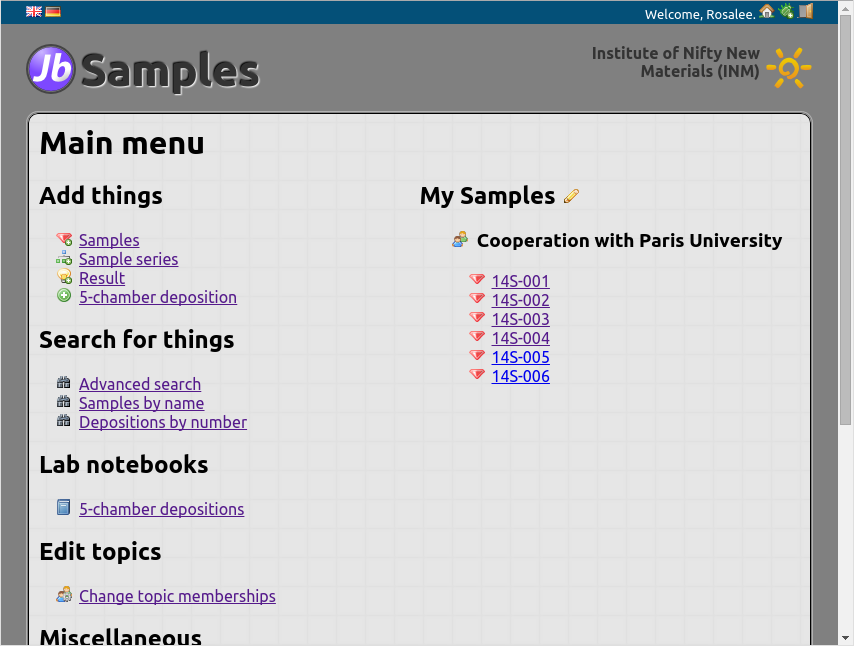
\includegraphics{ss_main.png}}}

Log in as \code{r.calvert}, the typical ordinary user.  We will see how she gets
her work done.

\index{My Samples}\index{main menu}\index{topics}\index{sample!series}\index{series!sample}

\subsection{The “My Samples” list}
\label{demo:the-my-samples-list}\label{demo:index-2}
In the main menu, you can see Rosalee's “My Samples” on the right hand side.
This list usually contains not \emph{all} samples of a user but only those that are
\emph{currently of interest} to him/her.  Still, this list may become quite long,
and is therefore structured by \emph{topics} and \emph{sample series}.  You may click on
the bullet icons (
\includegraphics{group.png} or 
\includegraphics{chart_organisation.png}) in the list to fold and
unfold sections that you want to hide.

\index{topics|textbf}

\subsection{Topics}
\label{demo:topics}\label{demo:index-3}
One sample usually belongs to exactly one topic.  This helps to organise
samples.  For one thing, one can give topics expressive names, which makes the
samples' purpose clear.  In Rosalee's list, all samples belong to the topic
“Cooperation with Paris University”.

\index{permissions}
But even more important is that topics define who can see the sample.  The
prime directive in JuliaBase is: \emph{You can only see samples of your topics.}

If a sample is in no topic, it is completely unprotected.  Everyone can see it
and take possession of it.  There may be use cases for that but usually, you
should put all your samples in topics.

People can be in an arbitrary lot of topics at the same time, but a sample is
in exactly one topic.  It may change it during its lifetime, though.  Senior
team members may have the permission to see all samples, whether in their
topics or not.  Sean Renard is such a person.

\index{sample!data sheet}\index{data sheet!sample}

\subsection{Sample data sheet}
\label{demo:sample-data-sheet}\label{demo:index-5}
{\hfill\scalebox{0.500000}{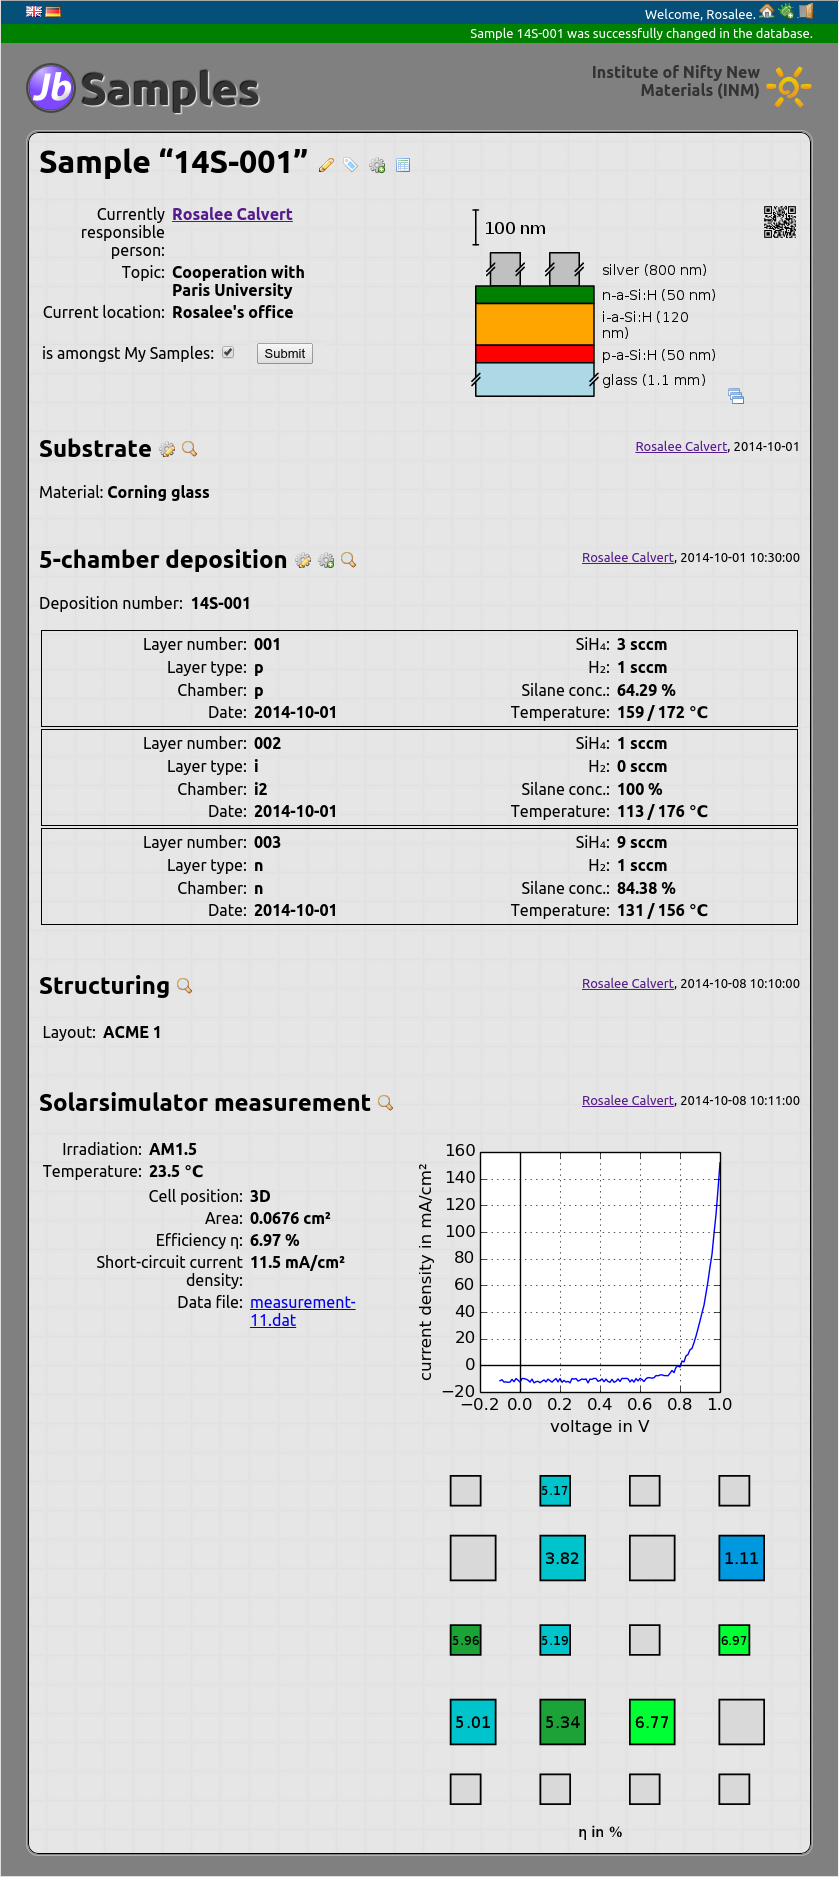
\includegraphics{ss_datasheet.png}}}

Let's visit a sample by clicking on “14S-001”.  You see its data sheet.  At the
top, it contains some general information like the currently responsible person
and the topic.  Then, you see a list of everything that has been done with this
sample, in chronological order.  It starts with the substrate, is continued
with the deposition of the silicon layers, and ends with a measurement in the
solar simulator.

\index{process}
Every such step is called a “process” in JuliaBase.  Even the “Substrate” is a
process, albeit a slightly odd one.  Every process has an operator and a
timestamp.  You can fold processes that would otherwise clobber the data sheet
by clicking on the heading.

The main work when adapting JuliaBase to a new institute is programming all the
processes that the institute needs.  The solarsimulator measurement at the
bottom is a good example why it is worth the effort.  Just click on the colored
squares, and you see how the data and the plot change immediately.  Such
features are lacking in off-the-shelf databases.  This high degree of
adaptability and flexibility is the primary strength of JuliaBase.

Let's scroll back to the top.  You see a schematic cross section of the sample,
called an “informal stack” because it may not be totally accurate.  This is not
part of JuliaBase's core because it may not be useful for every institute.  But
it's part of the source code and you may use it.  If you click on it, you get
it as a PDF.  This is also true for all plots in JuliaBase.

\index{sample!edit}\index{edit!sample}

\subsection{Edit samples}
\label{demo:edit-samples}
You can edit a sample by clicking on the pencil icon 
\includegraphics{pencil.png} next to the
sample's name.  “Editing a sample” refers \emph{only} to the data at the top of the
data sheet.  In particular, no processes are affected.  Very often when you
change somethin in JuliaBase, you have to describe your changes shortly at the
bottom right.  It may be tedious sometimes, but it may be very helpful to
others who get notified by your changes.


\subsection{Add processes}
\label{demo:add-processes}
Also on the top of the sample data sheet there is the gear icon 
\includegraphics{cog_add.png}, which is to append a new process to the sample.  If you click on it, you
are asked which kind of process you'd like to add.  Let's have a look at two
possibilities: Splitting and result process.

\index{sample!split}\index{split!sample}

\subsubsection{Split a sample}
\label{demo:split-a-sample}\label{demo:index-8}
If you split samples into pieces, you surely want to keep track of that.  For
doing so, you click on the gear icon 
\includegraphics{cog_add.png} and select “sample split”.
Then, you can enter the new names of the samples.  Usually, they extend their
parent's name.  When looking at a sample's data sheet, you also see all
processes of the parents.

\index{result}

\subsubsection{Result process}
\label{demo:index-9}\label{demo:result-process}
Result processes, often simply called “result”, are a handy ad-hoc way to
append something to a sample's data sheet.  If you want to add a measurement
result for which no dedicated process has been programmed so far, or if you
want to add a plot, a picture, or a comment, then create a result.  It's the
Swiss-Army-knife process if nothing else fits.  Because it's so flexible, be
careful not to have spelling errors in order to keep searching and exporting
easy.

\index{advanced!search}

\subsection{Advanced search}
\label{demo:advanced-search}\label{demo:index-10}
{\hfill\scalebox{0.500000}{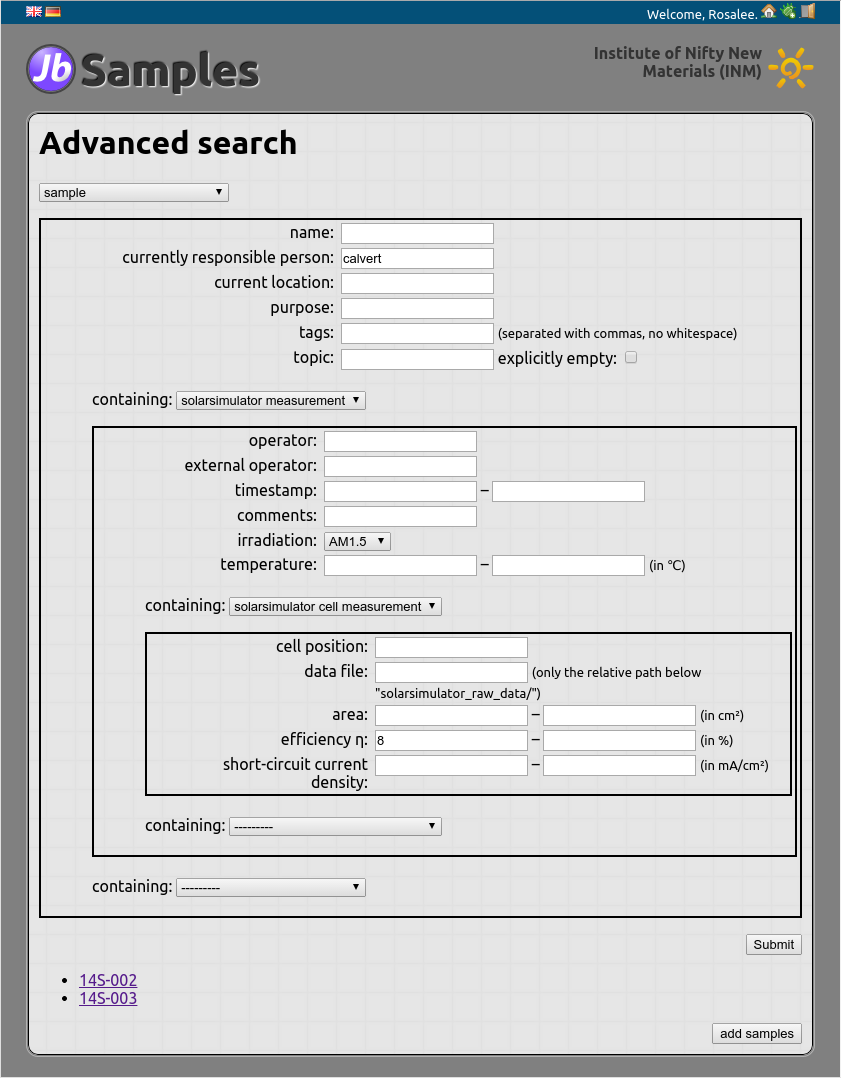
\includegraphics{ss_advanced_search.png}}}

Rosalee wants to see her best samples.  For this, go back to the main menu (the
house icon 
\includegraphics{house.png} on the top right, or the big text “Samples”) and select
“Search for things – Advanced search”.  Now, perform the following steps,
clicking on “Submit” after each step:
\begin{enumerate}
\item {} 
Select “sample” in the drop down menu.

\item {} 
Enter “calvert” in “currently responsible person” and select “solarsimulator
measurement” in the drop-down menu “containing”.

\item {} 
Select “AM1.5” in “irradiation”, and select “solarsimulator cell
measurement” in the inner drop-down menu “containing”.

\item {} 
Enter in “efficiency \(\eta\)“ the value “8”.

\end{enumerate}

You get the result as in the image next to this text: Two of her samples match
the criteria, namely “14S-002” and “14S-003”.  This means, both samples have at
least one solarsimulator measurement under AM 1.5 irradiation, with at least
one cell with an efficiency greater than 8\%.

\begin{notice}{note}{Note:}
You may bookmark advanced searches and revisit them as often as you wish.
Every time, you get new results for your old search criteria.
\end{notice}

\index{data!CSV export}\index{CSV!export, data}\index{export!data CSV}

\subsection{Data export}
\label{demo:data-export}\label{demo:index-11}
{\hfill\scalebox{0.500000}{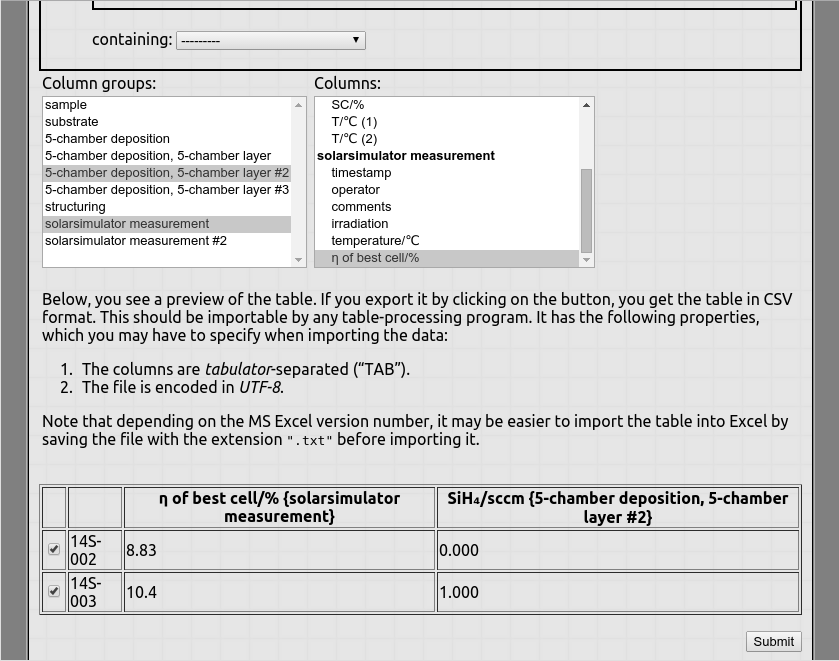
\includegraphics{ss_csv_export.png}}}

Rosalee needs the data in her spreadsheet program.  So, click yet another time
on “Submit”.  You may select the processes on the sample data sheet that should
be included into the output.  Select the second layer of the 5-chamber
deposition and the first solarsimulator measurement.  Click on “Submit”.  Now,
you may select the fields of these processes that should be included into the
output.  Select “\(\mathrm{SiH}_4\)/sccm” (the silane flux, by the way) of
the layer and “\(\eta\) of best cell/\%” of the solarsimulator measurement.  Click on
“Submit”.

The result is shown in the screenshot.  The table comprises all the data that
will be included into the output.  Click one last time on “Submit”, and you can
download that table as a CSV file ready-to-be-opened with your favourite
spreadsheet program.  When opening it, take care that columns are separated
\emph{only} by tabstops.

\index{add!sample}\index{sample!add}

\subsection{Add samples}
\label{demo:add-samples}\label{demo:index-12}
From the main menu, you can click on “Add things – Samples” to add samples.
Note that this page is quite institute-specific.  Your institute may not have
the concept of substrates, for example, and surely not something like a
“cleaning number”.  Anyway, you must enter the number of samples as well as
their current location.  Add a couple of samples, but don't rename them yet.

Fresh samples have a provisional name in JuliaBase.  It looks like “*00034”,
i.e., an asterisk followed by a five-digit number.  Never use these names on
sample boxes or in lab notebooks.  They are meant to be replaced by a real name
as quickly as possible.  Rosalee's samples get their names after the first
deposition of silicon, so let's do that now.

\index{lab notebook}

\subsection{Lab notebooks}
\label{demo:lab-notebooks}\label{demo:index-13}
From the main menu, open the lab notebook of the five-chamber deposition.  You
see six depositions of October 2014.  Select one of them.  JuliaBase shows you
a page containing the details of only this deposition.  At the top of it, click
on the gear icon 
\includegraphics{cog_add.png} in order to duplicate this deposition.


\subsection{Add new deposition process}
\label{demo:add-new-deposition-process}
Rosalee duplicates old depositions because she doesn't vary much.  This way,
she adds new depositions without fuss.  In the page for the new deposition, she
only has to select the samples for the deposition (which are the samples
recently added, with these “*…” names), change some other things that were
different in this run, and click on “Submit”.

{\hfill\scalebox{0.500000}{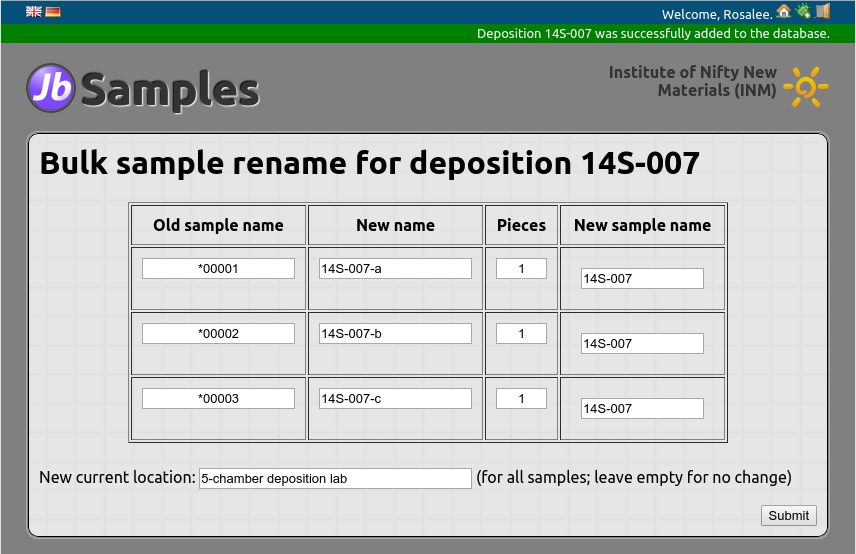
\includegraphics{ss_rename_after_depo.png}}}

Now, its a habit in the Institute of Nifty New Materials to give the sample the
same name as the deposition.  Therefore, immediately after having added the
deposition, you are redirected to a page where you can check and change the new
sample names.  JuliaBase suggests the deposition's name for all samples (in the
case of the screenshot, three of them).  However, names must be unique, so
Rosalee appends “…-a”, “…-b”, and “…-c” (see screenshot, second column).  Click
on “Submit”, that's it!  The newly deposited samples appear with their proper
names under “My Samples” on the main menu page.

Of course, your institute may have another workflow without such renaming,
which is a bad idea anyway – names in a database should never change.  So you
can just leave out the renaming page in your own code.

\index{permissions}

\subsection{Change permissions for processes}
\label{demo:permissions-to-processes}\label{demo:change-permissions-for-processes}\label{demo:index-14}
{\hfill\scalebox{0.500000}{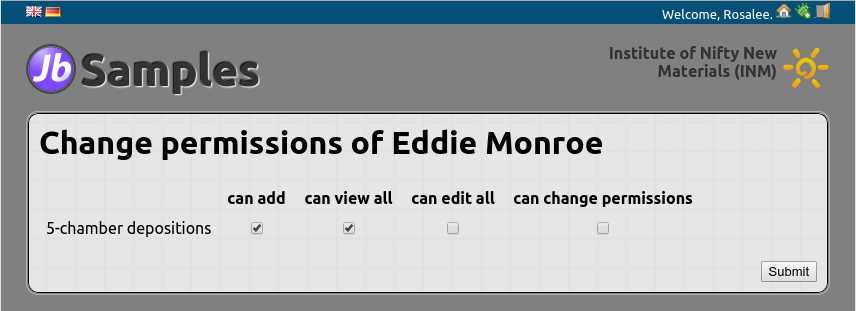
\includegraphics{ss_change_permissions.png}}}

As already mentioned, Rosalee is responsible for the 5-chamber deposition
setup.  But let's assume Eddie wants to do such depositions, too, and gets an
introduction?  Then, he should also be allowed to add such depositions to
JuliaBase.

Rosalee visits “Miscellaneous – Permissions to processes” from the main menu,
selects Eddie from the drop-down menu and clicks on “Submit”.  She puts tick
marks into the first two checkboxes and clicks again on “Submit”.  Now Eddie
has got the following additional permissions:
\begin{itemize}
\item {} 
He can add new 5-chamber depositions.

\item {} 
He can edit his own 5-chamber depositions (those that he's the operator of).

\item {} 
He can view all 5-chamber depositions.  In particular, this implies that he
can view the lab notebook.

\end{itemize}

\index{sample!claim}

\subsection{Claims of samples}
\label{demo:index-15}\label{demo:claims-of-samples}
There is one of Juliette's samples that Rosalee wants to acquire possession of.
In principle, Juliette could set the sample's “currently responsible person” to
Rosalee, but Juliette is reluctant to do work that also other could do (more on
that later).

Moreover, sometimes you must acquire possesion of orphaned samples; or of
samples that were imported as legacy data without any ownership information.
In these cases, it is really \emph{necessary} to be able to claim samples.  This is
done in two steps.

{\hfill\scalebox{0.500000}{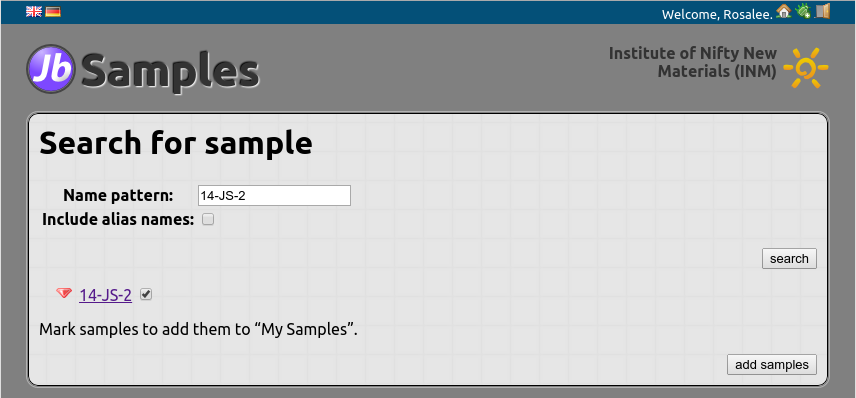
\includegraphics{ss_search_for_sample.png}}}


\subsubsection{Adding a sample to My Samples}
\label{demo:adding-a-sample-to-my-samples}
Rosalee clicks on “Search for things – Samples by name” in the main menu and
enters the name “14-JS-2” into the field.  She puts a tick into the checkbox
and clicks on “add samples”.  This way, the sample 14-JS-2 is added to
Rosalee's “My Samples”.


\subsubsection{The actual claim}
\label{demo:the-actual-claim}
{\hfill\scalebox{0.500000}{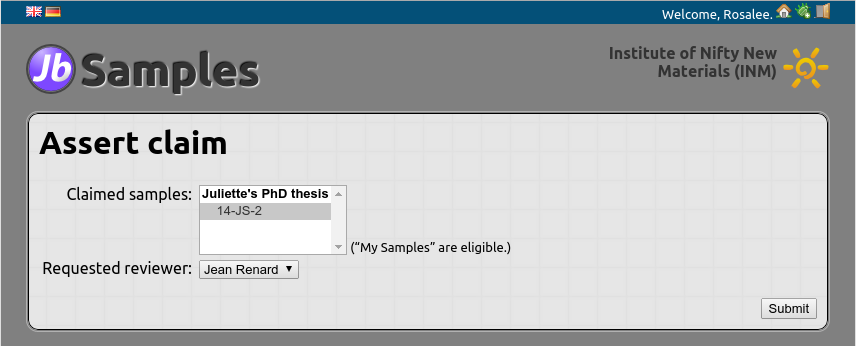
\includegraphics{ss_sample_claim.png}}}

Next, Rosalee visits “Miscellaneous – Sample claims” from the main menu, and on
the next page, selects “existing samples”.  Here, she selects 14-JS-2, and
“Sean Renard” as the reviewer of the claim (he's the only choice anyway).
That's it.  The next page lets Rosalee review the claim.  But now she has to
wait for Sean (who got an automatic email) for approving it.


\section{Juliette: The assigner of work}
\label{demo:juliette-the-assigner-of-work}
Juliette has a lot to do and cannot deal with such things as sample preparation
and characterization itself.  Thus, she assigns tasks to other people and
analyses the results.  Logout and re-login as j.silverton/12345.


\subsection{Adding a task}
\label{demo:adding-a-task}
{\hfill\scalebox{0.500000}{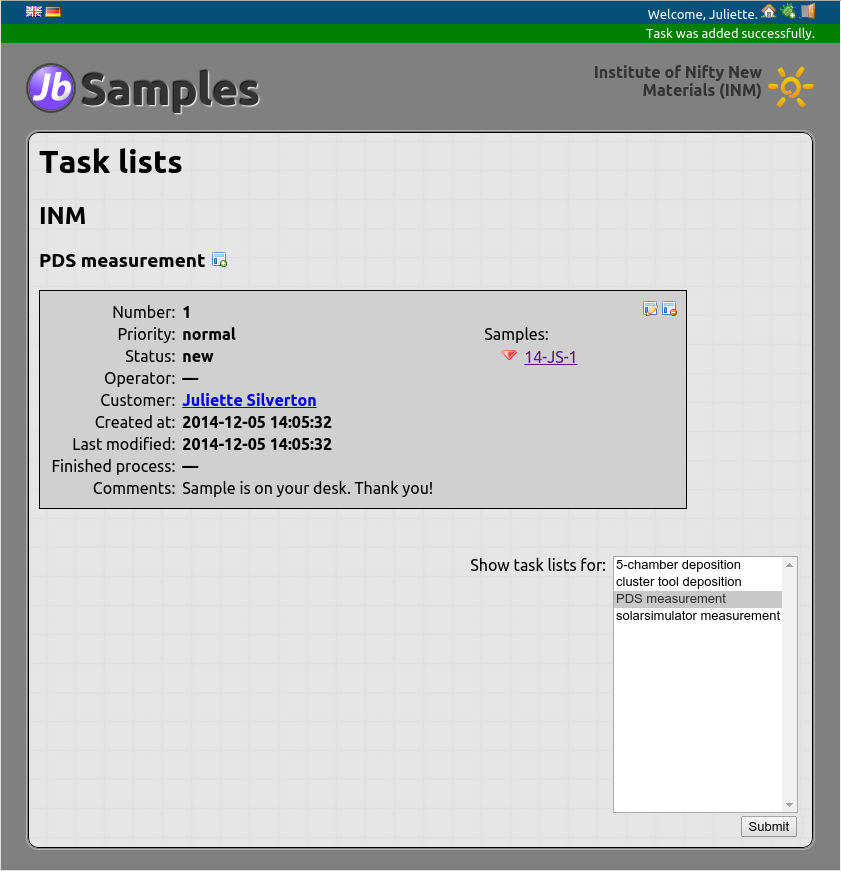
\includegraphics{ss_task_lists.png}}}

Let us assume Juliette wants to have a PDS measurement for her sample 14-JS-1.
Therefore, visit “Miscellaneous – Task lists” from the main menu.  There,
first set up the page by selecting the processes that you're interested in.
Select “PDS measurements” and click on “Submit”.

Now you add a new task for the PDS setup by clicking on the plus icon 
\includegraphics{layout_add.png} for PDS measurements.  Select the sample 14-JS-1, click on “Submit”
and you're finished.  You can see the new task in the list of tasks.  There,
you may withdraw it by clicking on the minus icon 
\includegraphics{layout_delete.png}, or edit
it by clicking on the pencil icon 
\includegraphics{layout_edit.png}.

\index{sample!send to user}\index{send to user!sample}

\subsection{Sending a sample to another user}
\label{demo:index-16}\label{demo:sending-a-sample-to-another-user}
{\hfill\scalebox{0.500000}{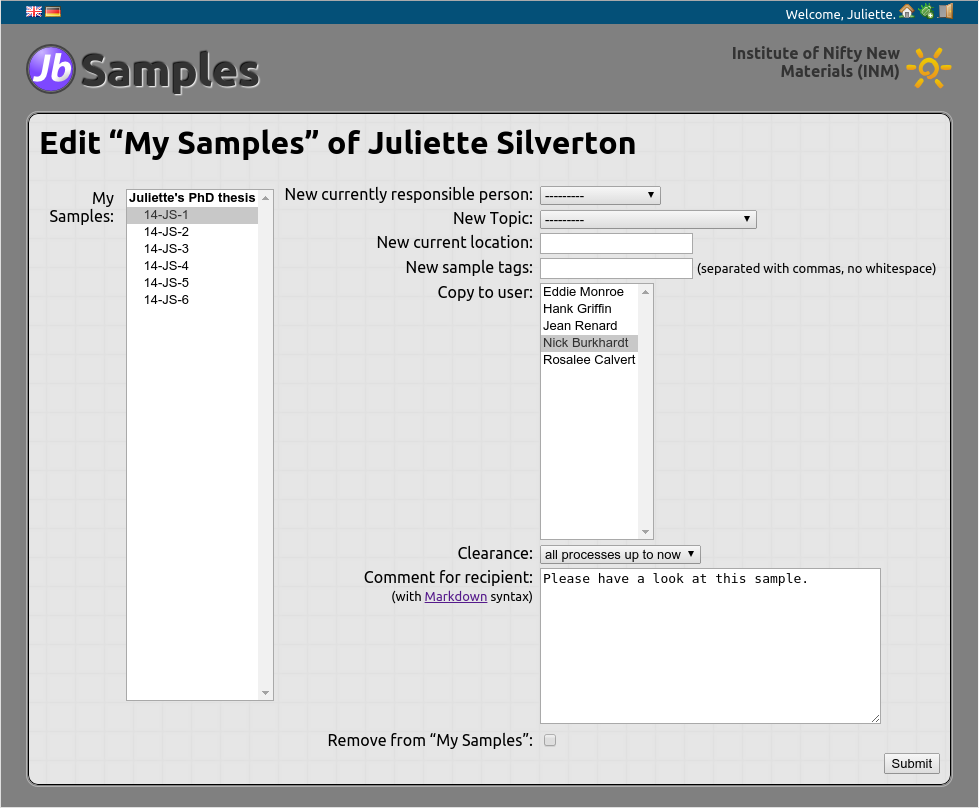
\includegraphics{ss_edit_my_samples.png}}}

Juliette wants to show the sample 14-JS-1 to Nick so that he can have a look at
it.  Of course, Nick could look for the sample himself, but since the sample is
in the topic “Juliette's PhD thesis” and Nick isn't, he cannot view the
sample's data sheet.

To send the sample to Nick, click on the pencil icon 
\includegraphics{pencil.png} next to “My
samples” on the main menu page.  Select the sample 14-JS-1 on the left.  Then,
on the right, select Nick in the multiple choice “Copy to user” and enter, say,
“Please have a look at this sample” at “Comment for recipient”.  Finally, set
“Clearance” to “all processes up to now”, because Juliette wants Nick to be
able to see the whole data sheet of 14-JS-1.


\section{Nick: Technical service for others}
\label{demo:nick-technical-service-for-others}
Now login as n.burkhardt/12345.  You can see 14-JS-1 under “My Samples”, and
you can view its data sheet.  The transfer has worked.

\index{newsfeed}\index{feed}\index{notifications}

\subsection{The newsfeed}
\label{demo:index-17}\label{demo:the-newsfeed}
Moreover, Nick has been notified by the transfer in “Main menu – Miscellaneous
– Newsfeed”.  There, he can also see that Juliette has files a new task for PDS
measurements because Nick has the necessary permissions for the PDS.  The
newsfeed contains all important news for the respective user: Changes in their
samples, new samples in their topics, samples transferred to them, new tasks,
and much more.

The newsfeed is not really intended to be view in the browser.  You may do so,
but it is a little bit awkward.  Rather, use a program capable of RSS feeds
like Thunderbird.  It is able to show you which entries in the feed are really
new.

\index{tasks}

\subsection{Tasks}
\label{demo:tasks}\label{demo:index-18}
{\hfill\scalebox{0.500000}{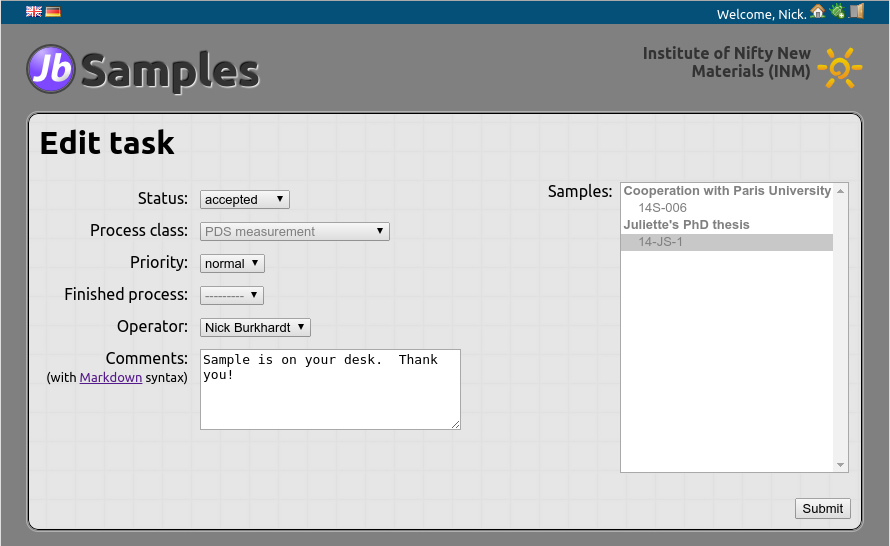
\includegraphics{ss_edit_task.png}}}

Since Nick has read that Juliette had filed a new PDS task, he visits the “Task
lists” page himself.  When doing this the first time, you have to select the
PDS and click on “Submit” to make PDS tasks viewable to Nick.

In general, there are more than one person working at a setup like the PDS.
Sometimes, people are absent (holidays, illness, etc).  Therefore, it is not
a-priori clear who will actually do a task, and the task must be explicitly
accepted by someone and assigned to someone.  In order to so this, click on the
pencil icon to edit it.  Set the “status” to “accepted” and “operator” to Nick
himself.  Juliette will get notified of this.

Nick can edit all PDS tasks by clicking on the pencil icon 
\includegraphics{layout_edit.png}.
When Nick is actually doing the measurement, he may set the task's status to
“in progress”, and after that, to “finished”.  A finished task may even be
connected with the concrete PDS measurement.

Some of these steps are optional.  It depends on your workflow.  An operator
might only set finished tasks to “finished” without further ado.  Or he may use
all of the features offered by task lists.  Or anything in between.


\section{Sean: The team leader}
\label{demo:sean-the-team-leader}
\index{permissions}
Login as s.renard/12345.  Sean, being the team leader, has extended
permissions.  They are:
\begin{itemize}
\item {} 
View all samples

\item {} 
Create new topics

\item {} 
Change memberships in all topics

\item {} 
Grant and revoke permissions to all setups

\item {} 
Approve or reject sample claims

\end{itemize}

The Institute of Nifty New Materials only has two levels: The team leader and
the rest.  You may add further levels in your institution, and you may set the
permissions in a different way.  However, we've made the experience that
complex permission policies are a burden that should be avoided.

\index{sample!claim}\index{claim!sample}

\subsection{Approve a sample claim}
\label{demo:approve-a-sample-claim}\label{demo:index-20}
{\hfill\scalebox{0.500000}{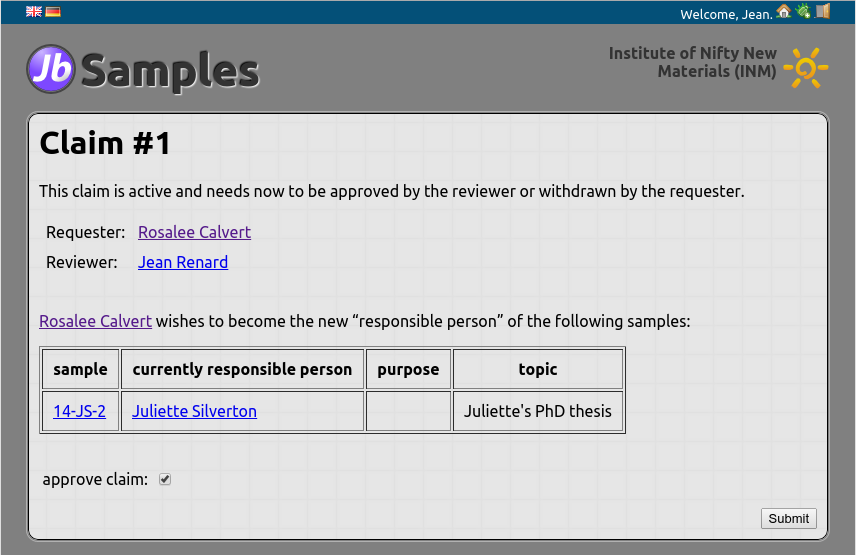
\includegraphics{ss_approve_claim.png}}}

Visit on the main menu “Miscellaneous – sample claims”.  At the bottom of this
page, you see the sample claim of Juliette.  Click on it.  Sean can now review
it in detail, and approve or reject it.

\index{installation}

\chapter{Installation}
\label{programming/installation:index-0}\label{programming/installation::doc}\label{programming/installation:installation}
\index{prerequisites}

\section{Prerequisites}
\label{programming/installation:prerequisites}\label{programming/installation:index-1}
Basically, you only need the current version of the \href{https://www.djangoproject.com/}{Django web framework}
together with its prerequisites.  Typically, this will be a computer with a
Linux operating system, and with Apache and PostgreSQL running on it.  However,
Django is flexible.  Is also runs on a Windows server, and it may be combined
with different webservers and database backends.  See \href{https://docs.djangoproject.com/en/1.7/topics/install/}{Django's own
installation guide} for more information.  Still, in this document, we assume
the default setup, which we also strongly recommend: Linux, Apache, PostgreSQL.
We deliberately avoid mentioning any particular Linux distribution because we
assume that at least their server flavours are similar enough.  For what it's
worth, the authors run Ubuntu Server.

Mostly, no sophisticated finetuning of the components is necessary because
JuliaBase deployments will serve only a few (\textless{} 1000) people.  In particular,
PostgreSQL and Apache can run in default configuration by and large.  On the
other hand, the computer should be a \href{http://linux-ha.org/}{high-availability system}, possibly
realized with virtual machines.  In our own installation, we manage a
three-nines system, i.e. 99.9 \% availability.  Additionally, regular backups
are a must! To set up these things, however, is beyond the scope of this
document.  Your IT department may turn out to be very helpful with this.

In the following, we'll show you how to get JuliaBase up and running quickly.
While our way is already useful for a production system, you may wish or need
to do it in a different way.  Thus, consider the following a good starting
point for your own configuration.


\section{Linux configuration}
\label{programming/installation:linux-configuration}
Additionally to the software that is running on any recent and decent Linux
operating system by default anyway, you must install:
\begin{itemize}
\item {} 
Apache2

\item {} 
PostgreSQL (and the Python module “psycopg2” for it)

\item {} 
memcached (and the Python module for it)

\item {} 
matplotlib

\item {} 
reportlab

\end{itemize}

\index{PostgreSQL!configuration}\index{configuration!PostgreSQL}

\section{PostgreSQL}
\label{programming/installation:postgresql}\label{programming/installation:index-2}
If you have PostgreSQL and Apache on the same computer, PostgreSQL's default
configuration should work for you.  The defaults are quite restrictive, so they
can be considered secure.  Otherwise, if you need to change something, it is
probably in pg\_hba.conf (where the \href{http://www.postgresql.org/docs/9.1/static/auth-methods.html}{user authentication} resides) or
postgresql.conf (where the \href{http://www.postgresql.org/docs/9.1/static/runtime-config.html}{general configuration} resides), both of which are
typically found in /etc/postgresql/\emph{version}/main/.

Anyway, you create a PostgreSQL user with this:

\begin{Verbatim}[commandchars=\\\{\},formatcom=\scriptsize]
\PYG{g+gp}{username@server:\PYGZti{}\PYGZdl{}} sudo \PYGZhy{}u postgres psql
\PYG{g+go}{psql (9.3.4)}
\PYG{g+go}{Type \PYGZdq{}help\PYGZdq{} for help.}

\PYG{g+go}{postgres=\PYGZsh{} CREATE USER username WITH PASSWORD ’topsecret’ CREATEDB;}
\PYG{g+go}{CREATE ROLE}
\PYG{g+go}{postgres=\PYGZsh{} \PYGZbs{}q}
\end{Verbatim}

In this snippet, you have to replace \code{username} with your UNIX user name, and
\code{topsecret} with a proper password, which shouldn't be your UNIX login
password.  Finally, create the database with:

\begin{Verbatim}[commandchars=\\\{\},formatcom=\scriptsize]
\PYG{g+gp}{username@server:\PYGZti{}\PYGZdl{}} createdb juliabase
\end{Verbatim}

\index{Django!configuration}\index{configuration!Django}

\section{Django}
\label{programming/installation:django}\label{programming/installation:index-3}
A certain version of JuliaBase works only with a certain version of Django.
Currently, this is Django 1.7.  Install it according to \href{https://www.djangoproject.com/download/}{Django's own
instructions}.  Not further configuration is necessary.


\section{JuliaBase}
\label{programming/installation:django-s-own-instructions}\label{programming/installation:juliabase}
JuliaBase is organized in a public \href{http://git-scm.com/}{Git} \href{https://github.com/juliabase}{repository on GitHub}.  So far,
there is no public release of JuliaBase 1.0.  However, the master branch in the
repository is a release candidate, which can be cloned locally with

\begin{Verbatim}[commandchars=\\\{\},formatcom=\scriptsize]
\PYG{g+gp}{username@server:\PYGZti{}\PYGZdl{}} git clone https://github.com/juliabase/juliabase.git
\end{Verbatim}

It contains three Django apps:
\begin{enumerate}
\item {} 
jb\_common

\item {} 
samples

\item {} 
institute

\end{enumerate}

“jb\_common” implements the basic JuliaBase functionality.  On top of that,
“samples” implements the actual samples database.  And on top of that,
“institute” implements code that is specific to the specific institution or
department or work group that wants to use JuliaBase.  “institute” implements a
\emph{generic} institute.  You will replace “institute” with your own app.

While the naked Git repo is suitable to get JuliaBase up and running quickly,
in the section {\hyperref[programming/programming:organizing-your-source-code]{\emph{“Organizing your source code”}}}, we'll explain the directory structure that you should use if you plan
to actually using JuliaBase.

\index{Apache!configuration}\index{configuration!Apache}

\section{Apache}
\label{programming/installation:index-4}\label{programming/installation:apache}
Add to your Apache configuration something like the following:

\begin{Verbatim}[commandchars=\\\{\},formatcom=\scriptsize]
\PYG{n+nt}{\PYGZlt{}VirtualHost} \PYG{l+s}{*:80}\PYG{n+nt}{\PYGZgt{}}
  \PYG{n+nb}{ServerName} juliabase.example.com
  \PYG{n+nb}{WSGIScriptAlias} / \PYG{l+s+sx}{/home/username/myproject/mysite/wsgi.py}
  \PYG{n+nb}{XSendFile} \PYG{k}{on}
  \PYG{n+nb}{XSendFilePath} /
  \PYG{n+nb}{Alias} \PYG{l+s+sx}{/media} \PYG{l+s+sx}{/var/www/juliabase/media}
  \PYG{n+nt}{\PYGZlt{}Location} \PYG{l+s}{\PYGZdq{}/\PYGZdq{}}\PYG{n+nt}{\PYGZgt{}}
    \PYG{n+nb}{Order} allow,deny
    \PYG{n+nb}{Allow} from \PYG{k}{all}
    \PYG{n+nb}{Require} \PYG{k}{all} granted
  \PYG{n+nt}{\PYGZlt{}/Location}\PYG{n+nt}{\PYGZgt{}}
\PYG{n+nt}{\PYGZlt{}/VirtualHost}\PYG{n+nt}{\PYGZgt{}}
\end{Verbatim}

This snippet contains several parts that highly probably need to be adjusted by
you, in particular \code{juliabase.example.com}, \code{username}, and all paths in
general.  But this should be obvious.  The proper place for it depends on your
Linux variant.  It may be the (new) file \code{/etc/apache2/httpd.conf}, or a new
file in \code{/etc/apache2/conf.d}, or a new file in
\code{/etc/apache2/sites-available} with a symlink in
\code{/etc/apache2/sites-enabled}.

\index{adapting}

\chapter{Programming}
\label{programming/programming:index-0}\label{programming/programming::doc}\label{programming/programming:programming}
This document explains JuliaBase for the programmer who wants to adapt it to
their institute, research department, or scientific group.  It contains an
overview of the process as a whole, and refers to other pages with the details.
We hope that it serves as a gentle tutorial which makes the adaption process as
easy as possible.  Feedback is welcomed!

For the adaption process, you should be familiar with several technologies:
\begin{enumerate}
\item {} 
\emph{Python}.  You should have advanced experience in this language.  This
includes the standard library; you should at least know what it can do and
how to find information about it.

\item {} 
\emph{Django}.  You must have mastered the tutorial of the Django web framework.

\item {} 
\emph{HTML}.  Basic knowledge should be enough.

\end{enumerate}

Furthermode, some admin skills are necessary to get everything running.

\index{source code!structure}\index{structure!source code}

\section{Organizing your source code}
\label{programming/programming:organizing-your-source-code}\label{programming/programming:index-1}\label{programming/programming:id1}
It would be a bad idea to download JuliaBase's source code and modify it
directly to your needs because then, any JuliaBase update would destroy your
changes.  Instead, you make a structure according to this:

\begin{Verbatim}[commandchars=\\\{\},formatcom=\scriptsize]
myproject/
    manage.py
    juliabase/
        \PYGZob{}the original JuliaBase release\PYGZcb{}
    mysite/
        \PYGZus{}\PYGZus{}init\PYGZus{}\PYGZus{}.py
        settings.py
        urls.py
        wsgi.py
    institute/
        \PYGZus{}\PYGZus{}init\PYGZus{}\PYGZus{}.py
        admin.py
        urls.py
        migrations/
        models/
        static/
        templates/
        views/
        ...
\end{Verbatim}

Thus, follow these steps:
\begin{enumerate}
\item {} 
Create the directory \code{myproject/}.  (Don't use Django's
\code{startproject} command here or in the following.)

\item {} 
Copy a JuliaBase release to \code{myproject/juliabase}

\item {} 
Copy the file \code{myproject/juliabase/manage.py} to \code{myproject/}.

\item {} 
Create \code{myproject/mysite/}

\item {} 
Copy the files \code{settings.py}, \code{urls.py}, and \code{wsgi.py}
from \code{myproject/juliabase/} to \code{myproject/mysite/}

\item {} 
Create an empty file \code{myproject/mysite/\_\_init\_\_.py}

\item {} 
Copy recursively the directory \code{myproject/juliabase/institute} to
\code{myproject/}.

\end{enumerate}

\index{git}

\subsection{Git subtree}
\label{programming/programming:git-subtree}\label{programming/programming:index-2}
If you're using Git, you may consider using the \code{subtree} command to get
JuliaBase in your repo: You structure your repository like above but without
the \code{juliabase} subdirectory.  Then, you say:

\begin{Verbatim}[commandchars=\\\{\},formatcom=\scriptsize]
\PYG{g+gp}{username@server:\PYGZti{}/myproject\PYGZdl{}} git subtree add \PYGZhy{}\PYGZhy{}prefix juliabase \PYGZhy{}\PYGZhy{}squash \PYG{l+s+se}{\PYGZbs{}}
\PYG{g+go}{    https://github.com/juliabase/juliabase.git v1.0}
\end{Verbatim}

A new version is pulled into your repo with:

\begin{Verbatim}[commandchars=\\\{\},formatcom=\scriptsize]
\PYG{g+gp}{username@server:\PYGZti{}/myproject\PYGZdl{}} git subtree pull \PYGZhy{}\PYGZhy{}prefix juliabase \PYGZhy{}\PYGZhy{}squash \PYG{l+s+se}{\PYGZbs{}}
\PYG{g+go}{    https://github.com/juliabase/juliabase.git v2.0}
\end{Verbatim}


\section{Creating a new Django app}
\label{programming/programming:creating-a-new-django-app}
Okay, now let's dive into the serious stuff.

You created your Django project, you added JuliaBase to it as explained in
{\hyperref[programming/programming:organizing-your-source-code]{Organizing your source code}}.  Furthermore, you set up everything as
explained in {\hyperref[programming/installation::doc]{\emph{Installation}}} (Apache is not yet needed).  Let's
try to get it running with

\begin{Verbatim}[commandchars=\\\{\},formatcom=\scriptsize]
\PYG{g+gp}{username@server:\PYGZti{}/myproject\PYGZdl{}} ./manage.py migrate
\PYG{g+gp}{username@server:\PYGZti{}/myproject\PYGZdl{}} ./manage.py loaddata demo\PYGZus{}accounts
\PYG{g+gp}{username@server:\PYGZti{}/myproject\PYGZdl{}} ./manage.py collectstatic
\PYG{g+gp}{username@server:\PYGZti{}/myproject\PYGZdl{}} ./manage.py runserver
\end{Verbatim}

This should make the site accessible locally at the URL \href{http://127.0.0.1:8000}{http://127.0.0.1:8000}.

The institute app that is used is \code{myproject/institute}.  For far, it is
a 1:1 copy of the JuliaBase app of the same name.  The plan is to transform it
into what \emph{you} need by pruning and modifying it.  The primary tasks when
adapting the app to your group or institution are:
\begin{enumerate}
\item {} 
Branding.

\item {} 
Adapting the “add new samples” page.

\item {} 
Manage the physical processes.

\end{enumerate}

\index{branding}

\subsection{Branding}
\label{programming/programming:branding}\label{programming/programming:index-3}
For the time being, we will stay with the app name “institute” to keep the
number of changes small.  Remember that it is only the app name; you may
re-brand the webpages to whatever you like.  The central point of doing so is
\code{institute/templates/jb\_base.html}.  There, you may change the name of
the institution as well as its logo.  The logo file should be placed in
\code{institute/static/institute/}.

Moreover, every JuliaBase installation must have at least one department.  It
needs to be created only once and should be named appropriately.

\index{sample!add}\index{add!sample}

\subsection{The “add new samples” view}
\label{programming/programming:index-4}\label{programming/programming:the-add-new-samples-view}
JuliaBase respects that creating new samples is a rather institute-specific
procedure and therefore does not include a view for this.  Instead, you must
create one, but you may use the INM's view in
\code{institute/views/samples/sample.py} as a comprehensive starting point (in
particular, the function \code{institute.views.samples.sample.add()}).

In the INM, every sample starts its life with a \emph{substrate}.  This is a
physical process that is always the very first one in the sample's history.
Therefore, the web page where you can add new samples also asks for the
substrate data, and creates the samples together with their substrates.  You
may or may not wish to have substrates, too.

The second big issue is sample names.  Most institutions have quite
idiosyncratic ideas about the sample naming policy.  But JuliaBase is very
flexible regarding this, see {\hyperref[programming/sample_names::doc]{\emph{Sample names}}}.  In the “add new samples”
view, you may let the user input (a pattern for) the new samples right away, or
you may give the names totally automatically.  Or, you may do it similarly to
the INM: Let the user decide between some options, and possibly redirect to a
bulk-rename view after having added the samples with provisional names.

\index{process}

\subsection{Physical processes}
\label{programming/programming:index-5}\label{programming/programming:physical-processes}
Physical processes are the thing that a JuliaBase programmer will spend most of
its time on.  They represent everything physically available in your
institution: Measurement setups, deposition setups, clean room processes,
chemical treatment, etc.

The INM app “institute” ships with some examples.  You may convert them to what
you need, but you can also remove them.  For the latter, visit
\code{institute/urls.py} and have a look at the following part (at the
bottom):

\begin{Verbatim}[commandchars=\\\{\},formatcom=\scriptsize]
\PYG{n}{pattern\PYGZus{}generator} \PYG{o}{=} \PYG{n}{PatternGenerator}\PYG{p}{(}\PYG{n}{urlpatterns}\PYG{p}{,} \PYG{l+s}{\PYGZdq{}}\PYG{l+s}{institute.views.samples}\PYG{l+s}{\PYGZdq{}}\PYG{p}{)}
\PYG{n}{pattern\PYGZus{}generator}\PYG{o}{.}\PYG{n}{deposition}\PYG{p}{(}\PYG{l+s}{\PYGZdq{}}\PYG{l+s}{ClusterToolDeposition}\PYG{l+s}{\PYGZdq{}}\PYG{p}{,} \PYG{n}{views}\PYG{o}{=}\PYG{p}{\PYGZob{}}\PYG{l+s}{\PYGZdq{}}\PYG{l+s}{add}\PYG{l+s}{\PYGZdq{}}\PYG{p}{,} \PYG{l+s}{\PYGZdq{}}\PYG{l+s}{edit}\PYG{l+s}{\PYGZdq{}}\PYG{p}{\PYGZcb{}}\PYG{p}{)}
\PYG{n}{pattern\PYGZus{}generator}\PYG{o}{.}\PYG{n}{deposition}\PYG{p}{(}\PYG{l+s}{\PYGZdq{}}\PYG{l+s}{FiveChamberDeposition}\PYG{l+s}{\PYGZdq{}}\PYG{p}{,} \PYG{l+s}{\PYGZdq{}}\PYG{l+s}{5\PYGZhy{}chamber\PYGZus{}depositions}\PYG{l+s}{\PYGZdq{}}\PYG{p}{)}
\PYG{n}{pattern\PYGZus{}generator}\PYG{o}{.}\PYG{n}{physical\PYGZus{}process}\PYG{p}{(}\PYG{l+s}{\PYGZdq{}}\PYG{l+s}{PDSMeasurement}\PYG{l+s}{\PYGZdq{}}\PYG{p}{,} \PYG{l+s}{\PYGZdq{}}\PYG{l+s}{number}\PYG{l+s}{\PYGZdq{}}\PYG{p}{)}
\PYG{n}{pattern\PYGZus{}generator}\PYG{o}{.}\PYG{n}{physical\PYGZus{}process}\PYG{p}{(}\PYG{l+s}{\PYGZdq{}}\PYG{l+s}{Substrate}\PYG{l+s}{\PYGZdq{}}\PYG{p}{,} \PYG{n}{views}\PYG{o}{=}\PYG{p}{\PYGZob{}}\PYG{l+s}{\PYGZdq{}}\PYG{l+s}{edit}\PYG{l+s}{\PYGZdq{}}\PYG{p}{\PYGZcb{}}\PYG{p}{)}
\PYG{n}{pattern\PYGZus{}generator}\PYG{o}{.}\PYG{n}{physical\PYGZus{}process}\PYG{p}{(}\PYG{l+s}{\PYGZdq{}}\PYG{l+s}{Structuring}\PYG{l+s}{\PYGZdq{}}\PYG{p}{,} \PYG{n}{views}\PYG{o}{=}\PYG{p}{\PYGZob{}}\PYG{l+s}{\PYGZdq{}}\PYG{l+s}{edit}\PYG{l+s}{\PYGZdq{}}\PYG{p}{\PYGZcb{}}\PYG{p}{)}
\PYG{n}{pattern\PYGZus{}generator}\PYG{o}{.}\PYG{n}{physical\PYGZus{}process}\PYG{p}{(}\PYG{l+s}{\PYGZdq{}}\PYG{l+s}{SolarsimulatorMeasurement}\PYG{l+s}{\PYGZdq{}}\PYG{p}{)}
\end{Verbatim}

Here, you can simply remove a line and the process is gone.  Well, not
entirely: You still need to remove its views module, templates, and models in
order to have everything neat and clean.  But removing the URL is enough for
the moment.

\index{add!process module}\index{process!module, add}\index{module!add process}

\section{Adding a new process module}
\label{programming/programming:index-6}\label{programming/programming:adding-a-new-process-module}
So you want to add a new measurement device or manufacturing process to your
JuliaBase installation.  You do so by adding new models, views, URLs, and
possibly an electronic lab notebook to your app “institute”.

I will show how to do that step-by-step.  In this example case, we write the
code for layer thickness measurements.


\subsection{Overview}
\label{programming/programming:overview}
The following steps are necessary for creating a physical process:
\begin{enumerate}
\item {} 
Create a database model in \code{institute/models.py}.

\item {} 
Create links in \code{urls.py}.

\item {} 
Create a view module in \code{samples/views/}.  Fill the view module with an
“EditView” class.

\item {} 
Create an “edit” and a “show” template in \code{templates/}.

\item {} 
\emph{(Optional)} Create an electronic lab notebook.

\item {} 
\emph{(Optional)} Create support for the new process in the Remote Client.

\item {} 
\emph{(Optional)} Import legacy data.

\end{enumerate}

In general, you will not do all of this from scratch.  Instead, you will
copy-and-paste from an already existing process which is as similar to the new
one as possible.


\subsection{Creating the database models}
\label{programming/programming:creating-the-database-models}
A “database model” or simply a “model” is a class in the Python code which
represents a table in the database.  It defines which things need to be stored
for every thickness measurement.  Since a model is a very Django-specific
construction, see the \href{https://docs.djangoproject.com/en/dev/topics/db/models/}{Django model documentation} for the details.

Let us assume that your thickness measurements need two fields: The measured
thickness and the method that was used to measure the thickness.  For the
method, you want to give the user the choice between five pre-set methods.

Thus, add the following code to your \code{models.py}:

\begin{Verbatim}[commandchars=\\\{\},formatcom=\scriptsize]
\PYG{n}{method\PYGZus{}choices}\PYG{o}{=}\PYG{p}{(}\PYG{p}{(}\PYG{l+s}{u\PYGZdq{}}\PYG{l+s}{profilers\PYGZam{}edge}\PYG{l+s}{\PYGZdq{}}\PYG{p}{,} \PYG{n}{\PYGZus{}}\PYG{p}{(}\PYG{l+s}{u\PYGZdq{}}\PYG{l+s}{profilers + edge}\PYG{l+s}{\PYGZdq{}}\PYG{p}{)}\PYG{p}{)}\PYG{p}{,}
                \PYG{p}{(}\PYG{l+s}{u\PYGZdq{}}\PYG{l+s}{ellipsometer}\PYG{l+s}{\PYGZdq{}}\PYG{p}{,} \PYG{n}{\PYGZus{}}\PYG{p}{(}\PYG{l+s}{u\PYGZdq{}}\PYG{l+s}{ellipsometer}\PYG{l+s}{\PYGZdq{}}\PYG{p}{)}\PYG{p}{)}\PYG{p}{,}
                \PYG{p}{(}\PYG{l+s}{u\PYGZdq{}}\PYG{l+s}{calculated}\PYG{l+s}{\PYGZdq{}}\PYG{p}{,} \PYG{n}{\PYGZus{}}\PYG{p}{(}\PYG{l+s}{u\PYGZdq{}}\PYG{l+s}{calculated from deposition parameters}\PYG{l+s}{\PYGZdq{}}\PYG{p}{)}\PYG{p}{)}\PYG{p}{,}
                \PYG{p}{(}\PYG{l+s}{u\PYGZdq{}}\PYG{l+s}{estimate}\PYG{l+s}{\PYGZdq{}}\PYG{p}{,} \PYG{n}{\PYGZus{}}\PYG{p}{(}\PYG{l+s}{u\PYGZdq{}}\PYG{l+s}{estimate}\PYG{l+s}{\PYGZdq{}}\PYG{p}{)}\PYG{p}{)}\PYG{p}{,}
                \PYG{p}{(}\PYG{l+s}{u\PYGZdq{}}\PYG{l+s}{other}\PYG{l+s}{\PYGZdq{}}\PYG{p}{,} \PYG{n}{\PYGZus{}}\PYG{p}{(}\PYG{l+s}{u\PYGZdq{}}\PYG{l+s}{other}\PYG{l+s}{\PYGZdq{}}\PYG{p}{)}\PYG{p}{)}\PYG{p}{)}

\PYG{k}{class} \PYG{n+nc}{ThicknessMeasurement}\PYG{p}{(}\PYG{n}{PhysicalProcess}\PYG{p}{)}\PYG{p}{:}
    \PYG{n}{thickness} \PYG{o}{=} \PYG{n}{models}\PYG{o}{.}\PYG{n}{DecimalField}\PYG{p}{(}\PYG{n}{\PYGZus{}}\PYG{p}{(}\PYG{l+s}{u\PYGZdq{}}\PYG{l+s}{layer thickness}\PYG{l+s}{\PYGZdq{}}\PYG{p}{)}\PYG{p}{,} \PYG{n}{max\PYGZus{}digits}\PYG{o}{=}\PYG{l+m+mi}{6}\PYG{p}{,}
                                    \PYG{n}{decimal\PYGZus{}places}\PYG{o}{=}\PYG{l+m+mi}{2}\PYG{p}{,} \PYG{n}{help\PYGZus{}text}\PYG{o}{=}\PYG{n}{\PYGZus{}}\PYG{p}{(}\PYG{l+s}{u\PYGZdq{}}\PYG{l+s}{in nm}\PYG{l+s}{\PYGZdq{}}\PYG{p}{)}\PYG{p}{)}
    \PYG{n}{method} \PYG{o}{=} \PYG{n}{models}\PYG{o}{.}\PYG{n}{CharField}\PYG{p}{(}\PYG{n}{\PYGZus{}}\PYG{p}{(}\PYG{l+s}{u\PYGZdq{}}\PYG{l+s}{measurement method}\PYG{l+s}{\PYGZdq{}}\PYG{p}{)}\PYG{p}{,} \PYG{n}{max\PYGZus{}length}\PYG{o}{=}\PYG{l+m+mi}{30}\PYG{p}{,}
                              \PYG{n}{choices}\PYG{o}{=}\PYG{n}{method\PYGZus{}choices}\PYG{p}{,} \PYG{n}{default}\PYG{o}{=}\PYG{l+s}{\PYGZdq{}}\PYG{l+s}{profilers\PYGZam{}edge}\PYG{l+s}{\PYGZdq{}}\PYG{p}{)}
\end{Verbatim}

The first part defines the five choices – note that it defines pairs of
strings, namely the internal name, which will be written to the hard disk, and
the descriptive name, which will be shown to the user.  The descriptive name is
enclosed by \code{\_(...)} to make it translatable to various languages.

Try to be as restrictive as is sensible when defining your models.  In
particular, mark only those fields as optional that are really optional, set
minimal and maximal values for numeric fields where applicable, and restrict
the number of digits for decimal fields.  This not only forces users to enter
plausible values, it also helps debugging.

\index{schema!migration}\index{migration!schema}

\subsubsection{Schema migration}
\label{programming/programming:index-7}\label{programming/programming:schema-migration}
After you add (or change) database models, you must to a so-called schema
migration.  This means that the tables in the database PostgreSQL are actually
changed, so that Django can use this new structure (a.k.a. schema).

It is a good idea to test a schema migration first on a test server.

The schema migration is created and applied by saying:

\begin{Verbatim}[commandchars=\\\{\},formatcom=\scriptsize]
./manage.py makemigrations institute
./manage.py migrate institute
\end{Verbatim}

The first line will create a new file in \code{institute/migrations/}.  It
should be added to your repository.

\index{URLs}

\subsection{Creating the URLs}
\label{programming/programming:creating-the-urls}\label{programming/programming:index-8}
The following work is done in \code{institute/urls.py}.  This step is fairly
simple.  For the thickness measurement, you add:

\begin{Verbatim}[commandchars=\\\{\},formatcom=\scriptsize]
\PYG{n}{pattern\PYGZus{}generator}\PYG{o}{.}\PYG{n}{physical\PYGZus{}process}\PYG{p}{(}\PYG{l+s}{\PYGZdq{}}\PYG{l+s}{LayerThicknessMeasurement}\PYG{l+s}{\PYGZdq{}}\PYG{p}{)}
\end{Verbatim}

\index{process!view}\index{view!process}

\subsection{Creating the view}
\label{programming/programming:creating-the-view}\label{programming/programming:index-9}
Typically, the view is the most complex task when creating a new kind of
process.  The Python file containing it must be called
\code{\emph{process\_class}.py}, thus in the current example,
\code{layer\_thickness\_measurement.py}.  It contains two parts:
\begin{enumerate}
\item {} 
The form(s).

\item {} 
The \code{class EditView} function.  This is mandatory.

\end{enumerate}


\subsubsection{The form}
\label{programming/programming:the-form}
For such a simple process class, this is simple:

\begin{Verbatim}[commandchars=\\\{\},formatcom=\scriptsize]
\PYG{k}{class} \PYG{n+nc}{LayerThicknessForm}\PYG{p}{(}\PYG{n}{samples}\PYG{o}{.}\PYG{n}{utils}\PYG{o}{.}\PYG{n}{views}\PYG{o}{.}\PYG{n}{ProcessForm}\PYG{p}{)}\PYG{p}{:}
    \PYG{k}{class} \PYG{n+nc}{Meta}\PYG{p}{:}
        \PYG{n}{model} \PYG{o}{=} \PYG{n}{LayerThicknessMeasurement}
        \PYG{n}{fields} \PYG{o}{=} \PYG{l+s}{\PYGZdq{}}\PYG{l+s}{\PYGZus{}\PYGZus{}all\PYGZus{}\PYGZus{}}\PYG{l+s}{\PYGZdq{}}
\end{Verbatim}


\subsubsection{View class}
\label{programming/programming:view-class}
You only need to create a view class for \emph{editing}, which can also be used to
\emph{adding}.  (The \emph{display} of an existing process is handled by JuliaBase.)
This view function must be defined like this:

\begin{Verbatim}[commandchars=\\\{\},formatcom=\scriptsize]
\PYG{k}{class} \PYG{n+nc}{EditView}\PYG{p}{(}\PYG{n}{ProcessView}\PYG{p}{)}\PYG{p}{:}
    \PYG{n}{form\PYGZus{}class} \PYG{o}{=} \PYG{n}{LayerThicknessForm}
\end{Verbatim}

For such a simple process like layer thickness measurement, that's it!  For
more complex processes, you may have to define further form classes, or do
additional validation in an \code{is\_referentially\_valid()} method in the
view class.  For the full API reference, see {\hyperref[programming/class-based_views::doc]{\emph{Class-based views}}}.  For
more examples, see the view modules of the \code{institute} app in JuliaBase's
source distribution.

\index{process!template}\index{template!process}

\subsection{Creating the templates}
\label{programming/programming:index-10}\label{programming/programming:creating-the-templates}
You need two templates per process, one that is called
\code{edit\_\emph{process\_name}.html} and the other that is called
\code{show\_\emph{process\_name}.html}.  Copy them from the process which is most
closely related to the one you're editing and apply the necessary
modifications.  Put them into the directory
\code{institute/templates/samples/}.


\section{A more complex example: Writing a deposition module}
\label{programming/programming:a-more-complex-example-writing-a-deposition-module}
I will show how to write a module for a deposition system by creating an
example module step-by-step.  The crucial difference to the simple measurement
process from above is that depositions consist of \emph{layers}, and there can be
arbitrarily many of them.  Every process class that needs some sort of
sub-model is more complicated, as explained in the following.


\subsection{The models}
\label{programming/programming:the-models}
A deposition system typically needs two models: One for the deposition data and
one for the layer data.  The layer data will carry much more fields than the
deposition, and it will contain a pointer to the deposition it belongs to.
This way, deposition and layers are kept together.  This pointer is represented
by a “foreign key” field.

The deposition model is derived from \code{Deposition},
which in turn is a \code{Process}:

\begin{Verbatim}[commandchars=\\\{\},formatcom=\scriptsize]
\PYG{k}{class} \PYG{n+nc}{FiveChamberDeposition}\PYG{p}{(}\PYG{n}{samples}\PYG{o}{.}\PYG{n}{models}\PYG{o}{.}\PYG{n}{Deposition}\PYG{p}{)}\PYG{p}{:}
    \PYG{k}{class} \PYG{n+nc}{Meta}\PYG{p}{(}\PYG{n}{samples}\PYG{o}{.}\PYG{n}{models}\PYG{o}{.}\PYG{n}{PhysicalProcess}\PYG{o}{.}\PYG{n}{Meta}\PYG{p}{)}\PYG{p}{:}
        \PYG{n}{permissions} \PYG{o}{=} \PYG{n}{generate\PYGZus{}permissions}\PYG{p}{(}
            \PYG{p}{\PYGZob{}}\PYG{l+s}{\PYGZdq{}}\PYG{l+s}{add}\PYG{l+s}{\PYGZdq{}}\PYG{p}{,} \PYG{l+s}{\PYGZdq{}}\PYG{l+s}{change}\PYG{l+s}{\PYGZdq{}}\PYG{p}{,} \PYG{l+s}{\PYGZdq{}}\PYG{l+s}{view\PYGZus{}every}\PYG{l+s}{\PYGZdq{}}\PYG{p}{,} \PYG{l+s}{\PYGZdq{}}\PYG{l+s}{edit\PYGZus{}permissions}\PYG{l+s}{\PYGZdq{}}\PYG{p}{\PYGZcb{}}\PYG{p}{,} \PYG{l+s}{\PYGZdq{}}\PYG{l+s}{FiveChamberDeposition}\PYG{l+s}{\PYGZdq{}}\PYG{p}{)}
\end{Verbatim}

It contains a full set of permissions to limit “add” and “edit” access to
certain users.  Moreover the \code{view\_every} makes a lab notebook possible.  See
{\hyperref[programming/permissions::doc]{\emph{Model permissions}}} for further information.

In contrast, the layer model is derived from \code{Layer},
which in turn is an ordinary Django model (not a \code{Process}):

\begin{Verbatim}[commandchars=\\\{\},formatcom=\scriptsize]
\PYG{k}{class} \PYG{n+nc}{FiveChamberLayer}\PYG{p}{(}\PYG{n}{samples}\PYG{o}{.}\PYG{n}{models}\PYG{o}{.}\PYG{n}{Layer}\PYG{p}{)}\PYG{p}{:}
    \PYG{n}{deposition} \PYG{o}{=} \PYG{n}{models}\PYG{o}{.}\PYG{n}{ForeignKey}\PYG{p}{(}
        \PYG{n}{FiveChamberDeposition}\PYG{p}{,} \PYG{n}{related\PYGZus{}name}\PYG{o}{=}\PYG{l+s}{\PYGZdq{}}\PYG{l+s}{layers}\PYG{l+s}{\PYGZdq{}}\PYG{p}{,} \PYG{n}{verbose\PYGZus{}name}\PYG{o}{=}\PYG{n}{\PYGZus{}}\PYG{p}{(}\PYG{l+s}{\PYGZdq{}}\PYG{l+s}{deposition}\PYG{l+s}{\PYGZdq{}}\PYG{p}{)}\PYG{p}{)}
    \PYG{n}{layer\PYGZus{}type} \PYG{o}{=} \PYG{n}{models}\PYG{o}{.}\PYG{n}{CharField}\PYG{p}{(}
        \PYG{n}{\PYGZus{}}\PYG{p}{(}\PYG{l+s}{\PYGZdq{}}\PYG{l+s}{layer type}\PYG{l+s}{\PYGZdq{}}\PYG{p}{)}\PYG{p}{,} \PYG{n}{max\PYGZus{}length}\PYG{o}{=}\PYG{l+m+mi}{2}\PYG{p}{,} \PYG{n}{choices}\PYG{o}{=}\PYG{n}{five\PYGZus{}chamber\PYGZus{}layer\PYGZus{}type\PYGZus{}choices}\PYG{p}{,} \PYG{n}{blank}\PYG{o}{=}\PYG{n+nb+bp}{True}\PYG{p}{)}
    \PYG{n}{chamber} \PYG{o}{=} \PYG{n}{models}\PYG{o}{.}\PYG{n}{CharField}\PYG{p}{(}
        \PYG{n}{\PYGZus{}}\PYG{p}{(}\PYG{l+s}{\PYGZdq{}}\PYG{l+s}{chamber}\PYG{l+s}{\PYGZdq{}}\PYG{p}{)}\PYG{p}{,} \PYG{n}{max\PYGZus{}length}\PYG{o}{=}\PYG{l+m+mi}{2}\PYG{p}{,} \PYG{n}{choices}\PYG{o}{=}\PYG{n}{five\PYGZus{}chamber\PYGZus{}chamber\PYGZus{}choices}\PYG{p}{)}
    \PYG{n}{sih4} \PYG{o}{=} \PYG{n}{model\PYGZus{}fields}\PYG{o}{.}\PYG{n}{DecimalQuantityField}\PYG{p}{(}
        \PYG{l+s}{\PYGZdq{}}\PYG{l+s}{SiH4}\PYG{l+s}{\PYGZdq{}}\PYG{p}{,} \PYG{n}{max\PYGZus{}digits}\PYG{o}{=}\PYG{l+m+mi}{7}\PYG{p}{,} \PYG{n}{decimal\PYGZus{}places}\PYG{o}{=}\PYG{l+m+mi}{3}\PYG{p}{,} \PYG{n}{unit}\PYG{o}{=}\PYG{l+s}{\PYGZdq{}}\PYG{l+s}{sccm}\PYG{l+s}{\PYGZdq{}}\PYG{p}{,} \PYG{n}{null}\PYG{o}{=}\PYG{n+nb+bp}{True}\PYG{p}{,} \PYG{n}{blank}\PYG{o}{=}\PYG{n+nb+bp}{True}\PYG{p}{)}
    \PYG{n}{h2} \PYG{o}{=} \PYG{n}{model\PYGZus{}fields}\PYG{o}{.}\PYG{n}{DecimalQuantityField}\PYG{p}{(}
        \PYG{l+s}{\PYGZdq{}}\PYG{l+s}{H2}\PYG{l+s}{\PYGZdq{}}\PYG{p}{,} \PYG{n}{max\PYGZus{}digits}\PYG{o}{=}\PYG{l+m+mi}{7}\PYG{p}{,} \PYG{n}{decimal\PYGZus{}places}\PYG{o}{=}\PYG{l+m+mi}{3}\PYG{p}{,} \PYG{n}{unit}\PYG{o}{=}\PYG{l+s}{\PYGZdq{}}\PYG{l+s}{sccm}\PYG{l+s}{\PYGZdq{}}\PYG{p}{,} \PYG{n}{null}\PYG{o}{=}\PYG{n+nb+bp}{True}\PYG{p}{,} \PYG{n}{blank}\PYG{o}{=}\PYG{n+nb+bp}{True}\PYG{p}{)}
    \PYG{n}{temperature\PYGZus{}1} \PYG{o}{=} \PYG{n}{model\PYGZus{}fields}\PYG{o}{.}\PYG{n}{DecimalQuantityField}\PYG{p}{(}
        \PYG{n}{\PYGZus{}}\PYG{p}{(}\PYG{l+s}{\PYGZdq{}}\PYG{l+s}{temperature 1}\PYG{l+s}{\PYGZdq{}}\PYG{p}{)}\PYG{p}{,} \PYG{n}{max\PYGZus{}digits}\PYG{o}{=}\PYG{l+m+mi}{7}\PYG{p}{,} \PYG{n}{decimal\PYGZus{}places}\PYG{o}{=}\PYG{l+m+mi}{3}\PYG{p}{,} \PYG{n}{unit}\PYG{o}{=}\PYG{l+s}{\PYGZdq{}}\PYG{l+s}{℃}\PYG{l+s}{\PYGZdq{}}\PYG{p}{,} \PYG{n}{null}\PYG{o}{=}\PYG{n+nb+bp}{True}\PYG{p}{,} \PYG{n}{blank}\PYG{o}{=}\PYG{n+nb+bp}{True}\PYG{p}{)}
    \PYG{n}{temperature\PYGZus{}2} \PYG{o}{=} \PYG{n}{model\PYGZus{}fields}\PYG{o}{.}\PYG{n}{DecimalQuantityField}\PYG{p}{(}
        \PYG{n}{\PYGZus{}}\PYG{p}{(}\PYG{l+s}{\PYGZdq{}}\PYG{l+s}{temperature 2}\PYG{l+s}{\PYGZdq{}}\PYG{p}{)}\PYG{p}{,} \PYG{n}{max\PYGZus{}digits}\PYG{o}{=}\PYG{l+m+mi}{7}\PYG{p}{,} \PYG{n}{decimal\PYGZus{}places}\PYG{o}{=}\PYG{l+m+mi}{3}\PYG{p}{,} \PYG{n}{unit}\PYG{o}{=}\PYG{l+s}{\PYGZdq{}}\PYG{l+s}{℃}\PYG{l+s}{\PYGZdq{}}\PYG{p}{,} \PYG{n}{null}\PYG{o}{=}\PYG{n+nb+bp}{True}\PYG{p}{,} \PYG{n}{blank}\PYG{o}{=}\PYG{n+nb+bp}{True}\PYG{p}{)}

    \PYG{k}{class} \PYG{n+nc}{Meta}\PYG{p}{(}\PYG{n}{samples}\PYG{o}{.}\PYG{n}{models}\PYG{o}{.}\PYG{n}{Layer}\PYG{o}{.}\PYG{n}{Meta}\PYG{p}{)}\PYG{p}{:}
        \PYG{n}{unique\PYGZus{}together} \PYG{o}{=} \PYG{p}{(}\PYG{l+s}{\PYGZdq{}}\PYG{l+s}{deposition}\PYG{l+s}{\PYGZdq{}}\PYG{p}{,} \PYG{l+s}{\PYGZdq{}}\PYG{l+s}{number}\PYG{l+s}{\PYGZdq{}}\PYG{p}{)}
\end{Verbatim}

The most important thing here is the \code{deposition} field which points to the
deposition this layer belongs to.  It forms part of a \code{unique\_together}
declaration.  The other fields are ordinary data fields.

\index{user context}\index{get\_context\_for\_user()}

\subsection{Populating user context}
\label{programming/programming:populating-user-context}\label{programming/programming:index-11}
In order to enable users to duplicate existing depositions, you should override
\code{get\_context\_for\_user()} method in the
deposition model:

\begin{Verbatim}[commandchars=\\\{\},formatcom=\scriptsize]
\PYG{k}{def} \PYG{n+nf}{get\PYGZus{}context\PYGZus{}for\PYGZus{}user}\PYG{p}{(}\PYG{n+nb+bp}{self}\PYG{p}{,} \PYG{n}{user}\PYG{p}{,} \PYG{n}{old\PYGZus{}context}\PYG{p}{)}\PYG{p}{:}
    \PYG{n}{context} \PYG{o}{=} \PYG{n}{old\PYGZus{}context}\PYG{o}{.}\PYG{n}{copy}\PYG{p}{(}\PYG{p}{)}
    \PYG{k}{if} \PYG{n}{permissions}\PYG{o}{.}\PYG{n}{has\PYGZus{}permission\PYGZus{}to\PYGZus{}add\PYGZus{}physical\PYGZus{}process}\PYG{p}{(}\PYG{n}{user}\PYG{p}{,} \PYG{n+nb+bp}{self}\PYG{o}{.}\PYG{n}{\PYGZus{}\PYGZus{}class\PYGZus{}\PYGZus{}}\PYG{p}{)}\PYG{p}{:}
        \PYG{n}{context}\PYG{p}{[}\PYG{l+s}{\PYGZdq{}}\PYG{l+s}{duplicate\PYGZus{}url}\PYG{l+s}{\PYGZdq{}}\PYG{p}{]} \PYG{o}{=} \PYG{l+s}{\PYGZdq{}}\PYG{l+s}{\PYGZob{}0\PYGZcb{}?copy\PYGZus{}from=\PYGZob{}1\PYGZcb{}}\PYG{l+s}{\PYGZdq{}}\PYG{o}{.}\PYG{n}{format}\PYG{p}{(}
            \PYG{n}{django}\PYG{o}{.}\PYG{n}{core}\PYG{o}{.}\PYG{n}{urlresolvers}\PYG{o}{.}\PYG{n}{reverse}\PYG{p}{(}\PYG{l+s}{\PYGZdq{}}\PYG{l+s}{add\PYGZus{}five\PYGZus{}chamber\PYGZus{}deposition}\PYG{l+s}{\PYGZdq{}}\PYG{p}{)}\PYG{p}{,}
            \PYG{n}{urlquote\PYGZus{}plus}\PYG{p}{(}\PYG{n+nb+bp}{self}\PYG{o}{.}\PYG{n}{number}\PYG{p}{)}\PYG{p}{)}
    \PYG{k}{else}\PYG{p}{:}
        \PYG{n}{context}\PYG{p}{[}\PYG{l+s}{\PYGZdq{}}\PYG{l+s}{duplicate\PYGZus{}url}\PYG{l+s}{\PYGZdq{}}\PYG{p}{]} \PYG{o}{=} \PYG{n+nb+bp}{None}
    \PYG{k}{return} \PYG{n+nb}{super}\PYG{p}{(}\PYG{n}{FiveChamberDeposition}\PYG{p}{,} \PYG{n+nb+bp}{self}\PYG{p}{)}\PYG{o}{.}\PYG{n}{get\PYGZus{}context\PYGZus{}for\PYGZus{}user}\PYG{p}{(}\PYG{n}{user}\PYG{p}{,} \PYG{n}{context}\PYG{p}{)}
\end{Verbatim}

This method is used when the HTML for a process (in this case a deposition) is
created.  Its return value is a dictionary which is combined with the
dictionary sent to the \code{show\_\emph{process\_class}.html} template.  This way,
additional program logic can be used to generate the HTML.  In case of
depositions, a “duplicate” button can be added, depending on the user's
permissions.


\subsection{The view}
\label{programming/programming:the-view}
In the view module which must be called \code{five\_chamber\_deposition.py}, the
main form gets additional cleaning methods:

\begin{Verbatim}[commandchars=\\\{\},formatcom=\scriptsize]
\PYG{k}{class} \PYG{n+nc}{DepositionForm}\PYG{p}{(}\PYG{n}{samples}\PYG{o}{.}\PYG{n}{utils}\PYG{o}{.}\PYG{n}{views}\PYG{o}{.}\PYG{n}{DepositionForm}\PYG{p}{)}\PYG{p}{:}

    \PYG{k}{class} \PYG{n+nc}{Meta}\PYG{p}{:}
        \PYG{n}{model} \PYG{o}{=} \PYG{n}{institute}\PYG{o}{.}\PYG{n}{models}\PYG{o}{.}\PYG{n}{FiveChamberDeposition}
        \PYG{n}{fields} \PYG{o}{=} \PYG{l+s}{\PYGZdq{}}\PYG{l+s}{\PYGZus{}\PYGZus{}all\PYGZus{}\PYGZus{}}\PYG{l+s}{\PYGZdq{}}

    \PYG{k}{def} \PYG{n+nf}{clean\PYGZus{}number}\PYG{p}{(}\PYG{n+nb+bp}{self}\PYG{p}{)}\PYG{p}{:}
        \PYG{n}{number} \PYG{o}{=} \PYG{n+nb}{super}\PYG{p}{(}\PYG{n}{DepositionForm}\PYG{p}{,} \PYG{n+nb+bp}{self}\PYG{p}{)}\PYG{o}{.}\PYG{n}{clean\PYGZus{}number}\PYG{p}{(}\PYG{p}{)}
        \PYG{k}{return} \PYG{n}{form\PYGZus{}utils}\PYG{o}{.}\PYG{n}{clean\PYGZus{}deposition\PYGZus{}number\PYGZus{}field}\PYG{p}{(}\PYG{n}{number}\PYG{p}{,} \PYG{l+s}{\PYGZdq{}}\PYG{l+s}{S}\PYG{l+s}{\PYGZdq{}}\PYG{p}{)}

    \PYG{k}{def} \PYG{n+nf}{clean}\PYG{p}{(}\PYG{n+nb+bp}{self}\PYG{p}{)}\PYG{p}{:}
        \PYG{n}{cleaned\PYGZus{}data} \PYG{o}{=} \PYG{n+nb}{super}\PYG{p}{(}\PYG{n}{DepositionForm}\PYG{p}{,} \PYG{n+nb+bp}{self}\PYG{p}{)}\PYG{o}{.}\PYG{n}{clean}\PYG{p}{(}\PYG{p}{)}
        \PYG{k}{if} \PYG{l+s}{\PYGZdq{}}\PYG{l+s}{number}\PYG{l+s}{\PYGZdq{}} \PYG{o+ow}{in} \PYG{n}{cleaned\PYGZus{}data} \PYG{o+ow}{and} \PYG{l+s}{\PYGZdq{}}\PYG{l+s}{timestamp}\PYG{l+s}{\PYGZdq{}} \PYG{o+ow}{in} \PYG{n}{cleaned\PYGZus{}data}\PYG{p}{:}
            \PYG{k}{if} \PYG{n}{cleaned\PYGZus{}data}\PYG{p}{[}\PYG{l+s}{\PYGZdq{}}\PYG{l+s}{number}\PYG{l+s}{\PYGZdq{}}\PYG{p}{]}\PYG{p}{[}\PYG{p}{:}\PYG{l+m+mi}{2}\PYG{p}{]} \PYG{o}{!=} \PYG{n}{cleaned\PYGZus{}data}\PYG{p}{[}\PYG{l+s}{\PYGZdq{}}\PYG{l+s}{timestamp}\PYG{l+s}{\PYGZdq{}}\PYG{p}{]}\PYG{o}{.}\PYG{n}{strftime}\PYG{p}{(}\PYG{l+s}{\PYGZdq{}}\PYG{l+s}{\PYGZpc{}}\PYG{l+s}{y}\PYG{l+s}{\PYGZdq{}}\PYG{p}{)}\PYG{p}{:}
                \PYG{n+nb+bp}{self}\PYG{o}{.}\PYG{n}{add\PYGZus{}error}\PYG{p}{(}\PYG{l+s}{\PYGZdq{}}\PYG{l+s}{number}\PYG{l+s}{\PYGZdq{}}\PYG{p}{,} \PYG{n}{\PYGZus{}}\PYG{p}{(}\PYG{l+s}{\PYGZdq{}}\PYG{l+s}{The first two digits must match the year of the deposition.}\PYG{l+s}{\PYGZdq{}}\PYG{p}{)}\PYG{p}{)}
        \PYG{k}{return} \PYG{n}{cleaned\PYGZus{}data}
\end{Verbatim}

The view class must override \code{get\_next\_id()} because the ID of a
deposition (its number) is non-numberical in the INM:

\begin{Verbatim}[commandchars=\\\{\},formatcom=\scriptsize]
\PYG{k}{class} \PYG{n+nc}{EditView}\PYG{p}{(}\PYG{n}{RemoveFromMySamplesMixin}\PYG{p}{,} \PYG{n}{DepositionView}\PYG{p}{)}\PYG{p}{:}
    \PYG{n}{form\PYGZus{}class} \PYG{o}{=} \PYG{n}{DepositionForm}
    \PYG{n}{layer\PYGZus{}form\PYGZus{}class} \PYG{o}{=} \PYG{n}{LayerForm}

    \PYG{k}{def} \PYG{n+nf}{get\PYGZus{}next\PYGZus{}id}\PYG{p}{(}\PYG{n+nb+bp}{self}\PYG{p}{)}\PYG{p}{:}
        \PYG{k}{return} \PYG{n}{institute}\PYG{o}{.}\PYG{n}{utils}\PYG{o}{.}\PYG{n}{base}\PYG{o}{.}\PYG{n}{get\PYGZus{}next\PYGZus{}deposition\PYGZus{}number}\PYG{p}{(}\PYG{l+s}{\PYGZdq{}}\PYG{l+s}{S}\PYG{l+s}{\PYGZdq{}}\PYG{p}{)}
\end{Verbatim}

\index{lab notebook}

\subsection{The lab notebook}
\label{programming/programming:index-12}\label{programming/programming:the-lab-notebook}
There are two things to set up for electronic lab notebooks: The URL and the
template.

Adding the URL for depositions is trivial as the method
{\hyperref[programming/utilities:samples.utils.urls.PatternGenerator.deposition]{\code{samples.utils.urls.PatternGenerator.deposition()}}} by default also
creates a lab notebook URL:

\begin{Verbatim}[commandchars=\\\{\},formatcom=\scriptsize]
\PYG{n}{pattern\PYGZus{}generator}\PYG{o}{.}\PYG{n}{deposition}\PYG{p}{(}\PYG{l+s}{\PYGZdq{}}\PYG{l+s}{FiveChamberDeposition}\PYG{l+s}{\PYGZdq{}}\PYG{p}{,} \PYG{l+s}{\PYGZdq{}}\PYG{l+s}{5\PYGZhy{}chamber\PYGZus{}depositions}\PYG{l+s}{\PYGZdq{}}\PYG{p}{)}
\end{Verbatim}

For normal processes, you need to request the lab notebook URL explicitly:

\begin{Verbatim}[commandchars=\\\{\},formatcom=\scriptsize]
\PYG{n}{pattern\PYGZus{}generator}\PYG{o}{.}\PYG{n}{physical\PYGZus{}process}\PYG{p}{(}\PYG{l+s}{\PYGZdq{}}\PYG{l+s}{ConductivityMeasurement}\PYG{l+s}{\PYGZdq{}}\PYG{p}{,}
                                   \PYG{n}{views}\PYG{o}{=}\PYG{p}{\PYGZob{}}\PYG{l+s}{\PYGZdq{}}\PYG{l+s}{add}\PYG{l+s}{\PYGZdq{}}\PYG{p}{,} \PYG{l+s}{\PYGZdq{}}\PYG{l+s}{edit}\PYG{l+s}{\PYGZdq{}}\PYG{p}{,} \PYG{l+s}{\PYGZdq{}}\PYG{l+s}{lab\PYGZus{}notebook}\PYG{l+s}{\PYGZdq{}}\PYG{p}{\PYGZcb{}}\PYG{p}{)}
\end{Verbatim}

Finally, you need to create a template called
\code{lab\_notebook\_\emph{process\_class}.html}.  It contains the processes to be
displayed in a lab notebook table in the context variable \code{processes}.


\section{Process glossary}
\label{programming/programming:process-glossary}\begin{description}
\item[{\index{process|textbf}process}] \leavevmode\phantomsection\label{programming/programming:term-process}
Anything that contains information about a sample.  This can be a process
in the literal meaning of the word, i.e. a deposition, an etching, a
clean room process etc.  It can also be a measurement or a result.
However, even the substrate, sample split, and sample death are
considered processes in JuliaBase.

It may have been better to call this “history item” or just “item”
instead of “process”.  The name “process” is due to merely historical
reasons, but there we go.

\item[{\index{measurement|textbf}measurement}] \leavevmode\phantomsection\label{programming/programming:term-measurement}
A special kind of \emph{process} which contains a single measurement.  It
belongs to the class of \emph{physical processes}.

\item[{\index{physical process|textbf}physical process}] \leavevmode\phantomsection\label{programming/programming:term-physical-process}
A deposition or a measurement process.  Its speciality is that only
people with the right permission for a certain physical process are
allowed to add and edit physical processes.

\item[{\index{result|textbf}result}] \leavevmode\phantomsection\label{programming/programming:term-result}
A result – or result process, as it is sometimes called in the source
code – is a special process which contains only a remark, a picture, or a
table with result values.

\end{description}

\index{permissions}

\chapter{Model permissions}
\label{programming/permissions:index-0}\label{programming/permissions::doc}\label{programming/permissions:model-permissions}
Permissions defined in the \code{Meta} class of models are used in Django to
define user permissions connected with this model.  JuliaBase also makes use of
this permissions framework.  There are, however, some peculiarities to be taken
into account when defining model permissions for JuliaBase model classes.


\section{Semantics and conventions}
\label{programming/permissions:semantics-and-conventions}
For models derived from \code{PhysicalProcess}, there are
four permissions with a special meaning to JuliaBase.  Their codenames must
follow the following naming conventions so that they have effect.

\index{process!unfinished}\index{unfinished!process}\begin{description}
\item[{\code{add\_\emph{classname}}}] \leavevmode
Means that a user is allowed to add new processes, and to edit unfinished
processes.

\item[{\code{edit\_permissions\_for\_\emph{classname}}}] \leavevmode
Means that a user is allowed to edit the permissions of other users for
this process class.

\item[{\code{view\_every\_\emph{classname}}}] \leavevmode
Means that a user is allowed to view all processes.  In particular, such
users are allowed to read the lab notebook.

\item[{\code{change\_\emph{classname}}}] \leavevmode
Means that a user is allowed to edit \emph{all} processes.

\end{description}

Further rules:
\begin{itemize}
\item {} 
\code{\emph{classname}} must be given in lowercase letters without underscores.

\item {} 
If a user has the permission \code{add\_\emph{classname}}, this user can edit
processes he/she is the operator of.

\item {} 
You can view processes of samples that you can view.

\item {} 
For obvious reasons, the \code{edit\_permissions\_for\_\emph{classname}} permission
implies all the others.  Usually, the users in charge of this setup or
apparatus have this permission.

\end{itemize}


\subsection{Example}
\label{programming/permissions:example}
The following code snipped defines the permissions for the
\code{ClusterToolDeposition}:

\begin{Verbatim}[commandchars=\\\{\},formatcom=\scriptsize]
\PYG{k}{class} \PYG{n+nc}{Meta}\PYG{p}{(}\PYG{n}{samples}\PYG{o}{.}\PYG{n}{models}\PYG{o}{.}\PYG{n}{PhysicalProcess}\PYG{o}{.}\PYG{n}{Meta}\PYG{p}{)}\PYG{p}{:}
    \PYG{n}{permissions} \PYG{o}{=} \PYG{p}{(}\PYG{p}{(}\PYG{l+s}{\PYGZdq{}}\PYG{l+s}{add\PYGZus{}clustertooldeposition}\PYG{l+s}{\PYGZdq{}}\PYG{p}{,} \PYG{l+s}{\PYGZdq{}}\PYG{l+s}{Can add cluster tool depositions}\PYG{l+s}{\PYGZdq{}}\PYG{p}{)}\PYG{p}{,}
                   \PYG{p}{(}\PYG{l+s}{\PYGZdq{}}\PYG{l+s}{edit\PYGZus{}permissions\PYGZus{}for\PYGZus{}clustertooldeposition}\PYG{l+s}{\PYGZdq{}}\PYG{p}{,}
                    \PYG{l+s}{\PYGZdq{}}\PYG{l+s}{Can edit perms for cluster tool I depositions}\PYG{l+s}{\PYGZdq{}}\PYG{p}{)}\PYG{p}{,}
                   \PYG{p}{(}\PYG{l+s}{\PYGZdq{}}\PYG{l+s}{view\PYGZus{}every\PYGZus{}clustertooldeposition}\PYG{l+s}{\PYGZdq{}}\PYG{p}{,}
                    \PYG{l+s}{\PYGZdq{}}\PYG{l+s}{Can view all cluster tool depositions}\PYG{l+s}{\PYGZdq{}}\PYG{p}{)}\PYG{p}{,}
                   \PYG{p}{(}\PYG{l+s}{\PYGZdq{}}\PYG{l+s}{change\PYGZus{}clustertooldeposition}\PYG{l+s}{\PYGZdq{}}\PYG{p}{,}
                    \PYG{l+s}{\PYGZdq{}}\PYG{l+s}{Can edit all cluster tool depositions}\PYG{l+s}{\PYGZdq{}}\PYG{p}{)}\PYG{p}{)}
\end{Verbatim}

Using {\hyperref[programming/utilities:jb_common.utils.base.generate_permissions]{\code{jb\_common.utils.base.generate\_permissions()}}}, this can be heavily
simplified:

\begin{Verbatim}[commandchars=\\\{\},formatcom=\scriptsize]
\PYG{k}{class} \PYG{n+nc}{Meta}\PYG{p}{(}\PYG{n}{samples}\PYG{o}{.}\PYG{n}{models}\PYG{o}{.}\PYG{n}{PhysicalProcess}\PYG{o}{.}\PYG{n}{Meta}\PYG{p}{)}\PYG{p}{:}
    \PYG{n}{permissions} \PYG{o}{=} \PYG{n}{generate\PYGZus{}permissions}\PYG{p}{(}
        \PYG{p}{\PYGZob{}}\PYG{l+s}{\PYGZdq{}}\PYG{l+s}{add}\PYG{l+s}{\PYGZdq{}}\PYG{p}{,} \PYG{l+s}{\PYGZdq{}}\PYG{l+s}{change}\PYG{l+s}{\PYGZdq{}}\PYG{p}{,} \PYG{l+s}{\PYGZdq{}}\PYG{l+s}{view\PYGZus{}every}\PYG{l+s}{\PYGZdq{}}\PYG{p}{,} \PYG{l+s}{\PYGZdq{}}\PYG{l+s}{edit\PYGZus{}permissions}\PYG{l+s}{\PYGZdq{}}\PYG{p}{\PYGZcb{}}\PYG{p}{,} \PYG{l+s}{\PYGZdq{}}\PYG{l+s}{ClusterToolDeposition}\PYG{l+s}{\PYGZdq{}}\PYG{p}{)}
\end{Verbatim}


\section{Omitting permissions}
\label{programming/permissions:omitting-permissions}
You may define all four permissions above.  However, if you omit some of them,
this has influence on JuliaBase's treatment of that process class.  The obvious
effect of omitting a permission is that no user can have that permission.  But
there are also more subtle effects.

If you omit the \code{add\_...} permission, \emph{every} user is allowed to add such a
process.  This may be suitable for things like specimen tempering, etching, or
thickness measurements that are not bound to a specific apparatus.

If you omit the \code{edit\_permissions\_for\_...} permission, the process class will
not appear in the {\hyperref[demo:permissions-to-processes]{\emph{“Permissions to processes”}}}
page.  Moreover, no email is sent to a person in charge of the setup if a user
creates his/her very first process of that kind.


\section{Django's default permissions}
\label{programming/permissions:django-s-default-permissions}
By default, Django generates an \code{add\_...}, \code{change\_...}, and \code{delete\_...}
permission for every model.  You can switch it off for a certain model by
saying

\begin{Verbatim}[commandchars=\\\{\},formatcom=\scriptsize]
\PYG{k}{class} \PYG{n+nc}{Meta}\PYG{p}{:}
    \PYG{n}{default\PYGZus{}permissions} \PYG{o}{=} \PYG{p}{(}\PYG{p}{)}
\end{Verbatim}

For physical processes, this has been done already — this is the reason why we
derived our \code{Meta} class from \code{samples.models.PhysicalProcess.Meta} in the
above {\hyperref[programming/permissions:example]{Example}}.

We recommend you to switch off Django's default permissions globally for your
project.  This way, it's much easier to control which permissions exist for a
certain model.  You switch them off by saying in your \code{manage.py}:

\begin{Verbatim}[commandchars=\\\{\},formatcom=\scriptsize]
\PYG{k+kn}{import} \PYG{n+nn}{django.contrib.auth.management}
\PYG{k}{def} \PYG{n+nf}{\PYGZus{}get\PYGZus{}only\PYGZus{}custom\PYGZus{}permissions}\PYG{p}{(}\PYG{n}{opts}\PYG{p}{,} \PYG{n}{ctype}\PYG{p}{)}\PYG{p}{:}
    \PYG{k}{return} \PYG{n+nb}{list}\PYG{p}{(}\PYG{n}{opts}\PYG{o}{.}\PYG{n}{permissions}\PYG{p}{)}
\PYG{n}{django}\PYG{o}{.}\PYG{n}{contrib}\PYG{o}{.}\PYG{n}{auth}\PYG{o}{.}\PYG{n}{management}\PYG{o}{.}\PYG{n}{\PYGZus{}get\PYGZus{}all\PYGZus{}permissions} \PYG{o}{=} \PYG{n}{\PYGZus{}get\PYGZus{}only\PYGZus{}custom\PYGZus{}permissions}
\end{Verbatim}


\chapter{Class-based views}
\label{programming/class-based_views:class-based-views}\label{programming/class-based_views::doc}
Class-based views are highly practical for the add/edit view of physical
processes because they keep code duplication at a minimum.  In some cases, you
get away with only a few lines of code.  Mixin classes reduce the redundancy
further.  Although it is still possible to have ordinary view \emph{functions} for
physical processes, we do not recommend this.  If you follow the convention of
calling your view class “\code{EditView}” and place it in a module called
\code{class\_name.py}, the {\hyperref[programming/utilities:samples.utils.urls.PatternGenerator]{\code{PatternGenerator}}}
will detect it and create the URL dispatch for it.


\section{The API}
\label{programming/class-based_views:the-api}
The API of JuliaBase's class-based view classes is best described by discussing
the attributes and methods of the common base class
{\hyperref[programming/class-based_views:samples.utils.views.class_views.ProcessWithoutSamplesView]{\code{ProcessWithoutSamplesView}}}.  Not
only if you derive your views, but also if you need to define your own
\emph{abstract} view class, you should derive it from one of the concrete classes
presented in the next section, though, because you probably want to re-use part
of their functionality.

This class is found in the module \code{samples.utils.views.class\_views}.
\index{ProcessWithoutSamplesView (class in samples.utils.views.class\_views)}

\begin{fulllineitems}
\phantomsection\label{programming/class-based_views:samples.utils.views.class_views.ProcessWithoutSamplesView}\pysiglinewithargsret{\strong{class }\bfcode{ProcessWithoutSamplesView}}{\emph{**kwargs}}{}
Abstract base class for the classed-based views.  It deals only with the
process per se, and in partuclar, with no samples associated with this
process.  This is done in the concrete derived classes
{\hyperref[programming/class-based_views:samples.utils.views.ProcessView]{\code{ProcessView}}} (one sample) and
\code{ProcessMultipleSamplesView} (multiple samples).  So, you should
never instantiate this one.

The methods that you most likely want to redefine in you own concrete class
are, with decreasing probability:
\begin{itemize}
\item {} 
\code{is\_referentially\_valid()}

\item {} 
\code{save\_to\_database()}

\item {} 
\code{get\_next\_id()}

\item {} 
\code{build\_forms()}

\item {} 
\code{get\_title()}

\item {} 
\code{get\_context\_data()}

\end{itemize}

Note that for \code{is\_referentially\_valid()},
\code{save\_to\_database()}, \code{build\_forms()}, and
\code{get\_context\_data()}, it is necessary to call the inherited method.

Since you connect forms with the view class, the view class expects certain
constructor signatures of the forms.  As for the process model form, it
must accept the logged-in user as the first argument.  This is the case for
{\hyperref[programming/utilities:samples.utils.views.ProcessForm]{\code{ProcessForm}}} and
{\hyperref[programming/utilities:samples.utils.views.DepositionForm]{\code{DepositionForm}}}, so this should not be a
problem.  The derived class (see below) may impose constrains on their
external forms either.
\begin{quote}\begin{description}
\item[{Variables}] \leavevmode\begin{itemize}
\item {} 
\textbf{form\_class} -- The model form class of the process of this view.

\item {} 
\textbf{model} -- The model class of the view.  If not given, it is derived from
the process form class.

\item {} 
\textbf{class\_name} -- The name of the model class,
e.g. \code{"clustertooldeposition"}.

\item {} 
\textbf{process} -- The process instance this view is about.  If we are about to
add a new process, this is \code{None} until the respective form is saved.

\item {} 
\textbf{forms} -- A dictionary mapping template context names to forms, or lists
of forms.  Mandatory keys in this dictionary are \code{"process"} and
\code{"edit\_description"}.  (Derived classes add \code{"sample"},
\code{"samples"}, \code{"remove\_from\_my\_samples"}, \code{"layers"}, etc.)

\item {} 
\textbf{data} -- The POST data if we have a POST request, or \code{None} otherwise.

\item {} 
\textbf{id} -- The ID of the process to edit, or \code{None} if we are about to add
a new one.  This is the recommended way to distinguish between editing
and adding.

\item {} 
\textbf{preset\_sample} -- The sample with which the process should be connected
by default.  May be \code{None}.

\item {} 
\textbf{request} -- The current request object.  This is inherited from Django's
view classes.

\item {} 
\textbf{template\_name} -- The file name of the rendering template, with the same
path syntax as in the \code{render()} function.

\item {} 
\textbf{identifying\_field} -- The name of the field in the process which is the
poor man's primary key for this process, e.g. the deposition number.  It
is taken from the model class.

\end{itemize}

\end{description}\end{quote}
\index{build\_forms() (ProcessWithoutSamplesView method)}

\begin{fulllineitems}
\phantomsection\label{programming/class-based_views:samples.utils.views.class_views.ProcessWithoutSamplesView.build_forms}\pysiglinewithargsret{\bfcode{build\_forms}}{}{}
Fills the \code{forms} dictionary with the forms, or lists of them.  In
this base class, we only add \code{"process"} itself and
\code{"edit\_description"}.  Note that the dictionary key is later used in
the template as context variable.

This method has no parameters and no return values, \code{self} is
modified in-situ.  It is good habit to check for a key before setting
it, allowing derived methods to set it themselves without doing double
work.

\end{fulllineitems}

\index{get\_context\_data() (ProcessWithoutSamplesView method)}

\begin{fulllineitems}
\phantomsection\label{programming/class-based_views:samples.utils.views.class_views.ProcessWithoutSamplesView.get_context_data}\pysiglinewithargsret{\bfcode{get\_context\_data}}{\emph{**kwargs}}{}
Generates the template context.  In particular, we inject the forms and the
title here into the context.  This method is part of the official
Django API.
\begin{quote}\begin{description}
\item[{Return}] \leavevmode
the context dict

\item[{Return type}] \leavevmode
dict

\end{description}\end{quote}

\end{fulllineitems}

\index{get\_next\_id() (ProcessWithoutSamplesView method)}

\begin{fulllineitems}
\phantomsection\label{programming/class-based_views:samples.utils.views.class_views.ProcessWithoutSamplesView.get_next_id}\pysiglinewithargsret{\bfcode{get\_next\_id}}{}{}
Gets the next identifying value for the process class.  In its default
implementation, it just takes the maximal existing value and adds 1.
This needs to be overridden if the identifying field is non-numeric.
\begin{quote}\begin{description}
\item[{Return}] \leavevmode
The next untaken of the identifying field, e.g. the next free
depostion number.

\item[{Return type}] \leavevmode
object

\end{description}\end{quote}

\end{fulllineitems}

\index{get\_title() (ProcessWithoutSamplesView method)}

\begin{fulllineitems}
\phantomsection\label{programming/class-based_views:samples.utils.views.class_views.ProcessWithoutSamplesView.get_title}\pysiglinewithargsret{\bfcode{get\_title}}{}{}
Creates the title of the response.  This is used in the \code{\textless{}title\textgreater{}}
tag and the \code{\textless{}h1\textgreater{}} tag at the top of the page.
\begin{quote}\begin{description}
\item[{Return}] \leavevmode
the title of the response

\item[{Return type}] \leavevmode
unicode

\end{description}\end{quote}

\end{fulllineitems}

\index{is\_all\_valid() (ProcessWithoutSamplesView method)}

\begin{fulllineitems}
\phantomsection\label{programming/class-based_views:samples.utils.views.class_views.ProcessWithoutSamplesView.is_all_valid}\pysiglinewithargsret{\bfcode{is\_all\_valid}}{}{}
Checks whether all forms are valid.  Unbound forms – which may occur also in
POST requests – are not checked.  Moreover, this method guarantees that
the \code{is\_valid()} method of every bound form is called in order
to collect all error messages.
\begin{quote}\begin{description}
\item[{Return}] \leavevmode
whether all forms are valid

\item[{Return type}] \leavevmode
bool

\end{description}\end{quote}

\end{fulllineitems}

\index{is\_referentially\_valid() (ProcessWithoutSamplesView method)}

\begin{fulllineitems}
\phantomsection\label{programming/class-based_views:samples.utils.views.class_views.ProcessWithoutSamplesView.is_referentially_valid}\pysiglinewithargsret{\bfcode{is\_referentially\_valid}}{}{}
Checks whether the data of all forms is consistent with each other
and with the database.  This is the partner of \code{is\_all\_valid()}
but checks the inter-relations of data.

This method is frequently overriden in concrete view classes.

Note that a \code{True} here does not imply a \code{True} from
\code{is\_all\_valid()}.  Both methods are independent of each other.
In particular, you must check the validity of froms that you use here.
\begin{quote}\begin{description}
\item[{Return}] \leavevmode
whether the data submitted to the view is valid

\item[{Return type}] \leavevmode
bool

\end{description}\end{quote}

\end{fulllineitems}

\index{save\_to\_database() (ProcessWithoutSamplesView method)}

\begin{fulllineitems}
\phantomsection\label{programming/class-based_views:samples.utils.views.class_views.ProcessWithoutSamplesView.save_to_database}\pysiglinewithargsret{\bfcode{save\_to\_database}}{}{}
Saves the data to the database.
\begin{quote}\begin{description}
\item[{Return}] \leavevmode
the saved process instance

\item[{Return type}] \leavevmode
\code{samples.models.PhysicalProcess}

\end{description}\end{quote}

\end{fulllineitems}

\index{startup() (ProcessWithoutSamplesView method)}

\begin{fulllineitems}
\phantomsection\label{programming/class-based_views:samples.utils.views.class_views.ProcessWithoutSamplesView.startup}\pysiglinewithargsret{\bfcode{startup}}{}{}
Fetch the process to-be-edited from the database and check permissions.
This method has no parameters and no return values, \code{self} is
modified in-situ.

\end{fulllineitems}


\end{fulllineitems}



\section{Main classes}
\label{programming/class-based_views:main-classes}
The following names are found in the module \code{samples.utils.views}.
\index{ProcessView (class in samples.utils.views)}

\begin{fulllineitems}
\phantomsection\label{programming/class-based_views:samples.utils.views.ProcessView}\pysiglinewithargsret{\strong{class }\bfcode{ProcessView}}{\emph{**kwargs}}{}
View class for physical processes with one sample each.  The HTML form for
the sample is called \code{sample} in the template.  Typical usage can be very
short:

\begin{Verbatim}[commandchars=\\\{\},formatcom=\scriptsize]
\PYG{k+kn}{from} \PYG{n+nn}{samples.utils.views} \PYG{k+kn}{import} \PYG{n}{ProcessForm}\PYG{p}{,} \PYG{n}{ProcessView}

\PYG{k}{class} \PYG{n+nc}{LayerThicknessForm}\PYG{p}{(}\PYG{n}{ProcessForm}\PYG{p}{)}\PYG{p}{:}
    \PYG{k}{class} \PYG{n+nc}{Meta}\PYG{p}{:}
        \PYG{n}{model} \PYG{o}{=} \PYG{n}{LayerThicknessMeasurement}
        \PYG{n}{fields} \PYG{o}{=} \PYG{l+s}{\PYGZdq{}}\PYG{l+s}{\PYGZus{}\PYGZus{}all\PYGZus{}\PYGZus{}}\PYG{l+s}{\PYGZdq{}}

\PYG{k}{class} \PYG{n+nc}{EditView}\PYG{p}{(}\PYG{n}{ProcessView}\PYG{p}{)}\PYG{p}{:}
    \PYG{n}{form\PYGZus{}class} \PYG{o}{=} \PYG{n}{LayerThicknessForm}
\end{Verbatim}

\end{fulllineitems}

\index{ProcessMultipleSamplesView (class in samples.utils.views)}

\begin{fulllineitems}
\phantomsection\label{programming/class-based_views:samples.utils.views.ProcessMultipleSamplesView}\pysiglinewithargsret{\strong{class }\bfcode{ProcessMultipleSamplesView}}{\emph{**kwargs}}{}
View class for physical processes with one or more samples each.  The HTML
form for the sample list is called \code{samples} in the template.  The usage
is analogous to {\hyperref[programming/class-based_views:samples.utils.views.ProcessView]{\code{ProcessView}}}.

\end{fulllineitems}

\index{DepositionView (class in samples.utils.views)}

\begin{fulllineitems}
\phantomsection\label{programming/class-based_views:samples.utils.views.DepositionView}\pysiglinewithargsret{\strong{class }\bfcode{DepositionView}}{\emph{**kwargs}}{}
View class for depositions.  The layers of the deposition must always be of
the same type.  If they are now, you must use
\code{DepositionMultipleTypeView} instead.  Additionally to
\code{form\_class}, you must set the \code{layer\_form\_class} class
variable to the form class to be used for the layers.

The layer form should be a subclass of {\hyperref[programming/class-based_views:samples.utils.views.SubprocessForm]{\code{SubprocessForm}}}.

\end{fulllineitems}

\index{DepositionMultipleTypeView (class in samples.utils.views)}

\begin{fulllineitems}
\phantomsection\label{programming/class-based_views:samples.utils.views.DepositionMultipleTypeView}\pysiglinewithargsret{\strong{class }\bfcode{DepositionMultipleTypeView}}{\emph{**kwargs}}{}
View class for depositions the layers of which are of different types (i.e.,
different models).  You can see it in action in the module
\code{institute.views.samples.cluster\_tool\_deposition}.  Additionally to
the class variable \code{form\_class}, you must set:
\begin{quote}\begin{description}
\item[{Variables}] \leavevmode\begin{itemize}
\item {} 
\textbf{layer\_form\_classes} -- This is a tuple of the form classes for the layers

\item {} 
\textbf{short\_labels} -- \emph{(optional)} This is a dict mapping a layer form class
to a concise name of that layer type.  It is used in the selection widget
of the add-layer form.

\end{itemize}

\end{description}\end{quote}

\end{fulllineitems}

\index{SubprocessForm (class in samples.utils.views)}

\begin{fulllineitems}
\phantomsection\label{programming/class-based_views:samples.utils.views.SubprocessForm}\pysiglinewithargsret{\strong{class }\bfcode{SubprocessForm}}{\emph{view}, \emph{*args}, \emph{**kwargs}}{}
Model form class for subprocesses and deposition layers.  Its only purpose
is to eat up the \code{view} parameter to the constructor so that you need not
redefine the constructor every time.

\end{fulllineitems}



\section{Mixins}
\label{programming/class-based_views:mixins}\index{RemoveFromMySamplesMixin (class in samples.utils.views)}

\begin{fulllineitems}
\phantomsection\label{programming/class-based_views:samples.utils.views.RemoveFromMySamplesMixin}\pysiglinewithargsret{\strong{class }\bfcode{RemoveFromMySamplesMixin}}{\emph{**kwargs}}{}
Mixin for views that like to offer a “Remove from my samples” button.  In
the template, they may add the following code:

\begin{Verbatim}[commandchars=\\\{\},formatcom=\scriptsize]
\PYG{p}{\PYGZob{}}\PYG{p}{\PYGZob{}} \PYG{n}{remove\PYGZus{}from\PYGZus{}my\PYGZus{}samples}\PYG{o}{.}\PYG{n}{as\PYGZus{}p} \PYG{p}{\PYGZcb{}}\PYG{p}{\PYGZcb{}}
\end{Verbatim}

This mixin must come before the main view class in the list of parents.

\end{fulllineitems}

\index{SubprocessesMixin (class in samples.utils.views)}

\begin{fulllineitems}
\phantomsection\label{programming/class-based_views:samples.utils.views.SubprocessesMixin}\pysiglinewithargsret{\strong{class }\bfcode{SubprocessesMixin}}{\emph{**kwargs}}{}
Mixing for views that represent processes with subprocesses.  Have a look at
\code{institute.views.samples.solarsimulator\_measurement} for an
example.  For this to work, you must define the followin additional class
variables:
\begin{itemize}
\item {} 
\code{subform\_class}: the model form class for the subprocesses

\item {} 
\code{process\_field}: the name of the field of the parent process in
the subprocess model

\item {} 
\code{subprocess\_field}: the \code{related\_name} parameter in the field
of the parent process in the subprocess model

\end{itemize}

You should derive the model form class of the subprocess from
{\hyperref[programming/class-based_views:samples.utils.views.SubprocessForm]{\code{SubprocessForm}}}.  This is not mandatory but
convenient, see there.

In the template, the forms of the subprocesses are available in a list
called \code{subprocesses}.  Furthermore, you should include

\begin{Verbatim}[commandchars=\\\{\},formatcom=\scriptsize]
\PYG{p}{\PYGZob{}}\PYG{p}{\PYGZob{}} \PYG{n}{number}\PYG{o}{.}\PYG{n}{as\PYGZus{}p} \PYG{p}{\PYGZcb{}}\PYG{p}{\PYGZcb{}}
\end{Verbatim}

in the template so that the user can set the number of subprocesses.

This mixin must come before the main view class in the list of parents.

\end{fulllineitems}


\index{remote client}

\chapter{The remote client}
\label{programming/remote_client:index-0}\label{programming/remote_client::doc}\label{programming/remote_client:the-remote-client}
The “remote client” is a programming library for contacting JuliaBase over the
network.  Being a library, it is not a program per se but used by your own code
for the bidirectional communication with the database.  The remote client
communicates through a REST HTTP interface implemented in the JuliaBase server.
This interface could be used directly, however, the remote client makes it much
easier.

In the following, we will describe what the remote client can do and how to get
it running.  For the API itself, we have to refer to the documentation in the
sources of the Python files in \code{remote\_client/}.  Note especially the
examples in \code{remote\_client/examples/}.


\section{Use cases}
\label{programming/remote_client:use-cases}
The remote client has many applications.

\index{crawlers}

\subsection{Crawlers}
\label{programming/remote_client:crawlers}\label{programming/remote_client:index-1}
Crawlers are programs that go through a bunch of data or log files and transmit
their content to the database.  For example, a measurement setup may write a
data file for every measurement run.  Every hour, a crawler is called, which
scans for new files.  It reads the new files and uses the content to add new
measurements processes to the database.  This way, new measurements
automatically end up in the database.  You may have more than one crawler
regularly running in your institute.

The very same crawler can also be used to import legacy data.  The crawler can
be programmed in such a way that during its first run, it imports thousands of
data sets of recent years, and from there on, it imports newly added data sets
every hour.

Since crawlers run unattendedly, they must be very robust.  If a data file is
invalid, or if the central server is temporarily unavailable, it must gently
exit and try again next time, without forgetting to add something, and without
adding things twice.

Moreover, legacy data mostly is poorly structured and organized.  If you think
your data is the exception, think again.  During writing the crawler, you will
be surprised how many odd ideas and mistakes your colleagues are capable of.

Be that as it may, crawlers are the primary use case for the remote client.
The remote client contains functions especially for making writing them as easy
as possible.


\subsection{Connecting the setup with the database}
\label{programming/remote_client:connecting-the-setup-with-the-database}
A more direct way than the crawler for bringing processing and measurement data
into the database, albeit not always feasible, is to extend the control program
of the experimental setup.  For this, you must have access to the source code
of the control program.  Then, you can use the remote client for writing new
runs immediately into the database.

However, the communication needn't be one-way.  You can also use the remote
client to authenticate the user, to check whether he or she is allowed to use
this setup, and to check whether the sample names belong to valid and for the
user accessible samples.

The remote client is written in Python, however, it is easy to use it from
programs written in other programming languages, and JuliaBase ships with a
Delphi binding.


\subsection{Data mining and analysis}
\label{programming/remote_client:data-mining-and-analysis}
Everyone with browser access to the JuliaBase database can use the remote
client for accessing, too.  The permissions will be the same in both cases, of
course.  This can be used by researchers capable of programming to get data
from the database and do something with it, e.g. creating statistics or
evaluating raw data.

Imagine the following: A researcher makes many sample series and measures their
temperature-dependent conductivity.  The researcher can write a program that
extracts the names of the raw data files from the database, then creates a plot
for each sample series with the conductivity curves of all samples of that
series, and writes these plots back to the database.  There, one can see them
on the series' pages, and in every sample's data sheet.


\section{Extending the remote client}
\label{programming/remote_client:extending-the-remote-client}
As for JuliaBase itself, also the remote client should be extended with the
functionality special to your institution.  This is not absolutely necessary,
but without it, you can only use the very basic functionality.  However,
extending the remote client is \emph{much} easier than extending JuliaBase.
\phantomsection\label{programming/remote_client:remote-client-file-list}
In JuliaBases' source code, the default remote client resides in the directory
\code{remote\_client/}, and it has the following structure:

\begin{Verbatim}[commandchars=\\\{\},formatcom=\scriptsize]
remote\PYGZus{}client/
    jb\PYGZus{}remote\PYGZus{}inm.py
    jb\PYGZus{}remote/
        \PYGZus{}\PYGZus{}init\PYGZus{}\PYGZus{}.py
        common.py
        samples.py
        settings.py
        ...
\end{Verbatim}

Replace the file \code{jb\_remote\_inm.py} with your own institute's code,
and give your file a name derived from your institution's name.  Your file
should start with something like:

\begin{Verbatim}[commandchars=\\\{\},formatcom=\scriptsize]
\PYG{k+kn}{from} \PYG{n+nn}{\PYGZus{}\PYGZus{}future\PYGZus{}\PYGZus{}} \PYG{k+kn}{import} \PYG{n}{absolute\PYGZus{}import}
\PYG{k+kn}{from} \PYG{n+nn}{jb\PYGZus{}remote} \PYG{k+kn}{import} \PYG{o}{*}

\PYG{n}{settings}\PYG{o}{.}\PYG{n}{ROOT\PYGZus{}URL} \PYG{o}{=} \PYG{n}{settings}\PYG{o}{.}\PYG{n}{TESTSERVER\PYGZus{}ROOT\PYGZus{}URL} \PYG{o}{=} \PYG{l+s}{\PYGZdq{}}\PYG{l+s}{https://juliabase.my\PYGZhy{}institute.edu/}\PYG{l+s}{\PYGZdq{}}
\end{Verbatim}

From there on, you are totally free how to program your incarnation of the
remote client.  You may use \code{jb\_remote\_inm.py} as a source of
inspiration, of course.


\subsection{Settings}
\label{programming/remote_client:settings}
The following settings in the remote client are available and should be set in
your \code{jb\_remote\_inm.py}:
\begin{description}
\item[{\code{ROOT\_URL}}] \leavevmode
The URL of the production server.  It must end in a slash.  Default: \code{None}

\item[{\code{TESTSERVER\_ROOT\_URL}}] \leavevmode
The URL of the test server.  It must end in a slash.  Default:
\code{"https://demo.juliabase.org/"}

\item[{\code{SMTP\_SERVER}}] \leavevmode
The DNS name of the SMTP server used for outgoing mail.  It may be used in
crawlers to send success or error emails.  You may add a port number after a
colon.  Default: \code{"mailrelay.example.com:587"}

\item[{\code{SMTP\_LOGIN}}] \leavevmode
The login name of the SMTP server.  If empty, no login is performed.  If not
empty, TLS is used.  Default: \code{"username"}

\item[{\code{SMTP\_PASSWORD}}] \leavevmode
The password used to login to the SMTP server through TLS.  Default:
\code{"password"}

\item[{\code{EMAIL\_FROM}}] \leavevmode
The sender used for outgoing mails.  Default: \code{"me@example.com"}

\item[{\code{EMAIL\_TO}}] \leavevmode
The recipient of outgoing mails.  Default: \code{"admins@example.com"}

\end{description}


\section{Local installation and usage}
\label{programming/remote_client:local-installation-and-usage}
Once you finished extending the default remote client, \emph{your} remote client
consists of the files listed {\hyperref[programming/remote_client:remote-client-file-list]{\emph{above}}}, with
\code{jb\_remote\_inm.py} substituted by your file called, say,
\code{jb\_remote\_my\_institute.py}.  This set of files needs to be copied to the machines
where the remote client is supposed to be used, and the top directory (the one
with your \code{jb\_remote\_my\_institute.py}) should be in \index{PYTHONPATH}\index{environment variable!PYTHONPATH}\code{PYTHONPATH}.

Then, you use the remote client with a Python script as easy as this:

\begin{Verbatim}[commandchars=\\\{\},formatcom=\scriptsize]
\PYG{k+kn}{from} \PYG{n+nn}{jb\PYGZus{}remote\PYGZus{}my\PYGZus{}institute} \PYG{k+kn}{import} \PYG{o}{*}

\PYG{n}{setup\PYGZus{}logging}\PYG{p}{(}\PYG{l+s}{\PYGZdq{}}\PYG{l+s}{console}\PYG{l+s}{\PYGZdq{}}\PYG{p}{)}
\PYG{n}{login}\PYG{p}{(}\PYG{l+s}{\PYGZdq{}}\PYG{l+s}{juliabase}\PYG{l+s}{\PYGZdq{}}\PYG{p}{,} \PYG{l+s}{\PYGZdq{}}\PYG{l+s}{12345}\PYG{l+s}{\PYGZdq{}}\PYG{p}{)}

\PYG{n}{sample} \PYG{o}{=} \PYG{n}{Sample}\PYG{p}{(}\PYG{l+s}{\PYGZdq{}}\PYG{l+s}{14\PYGZhy{}JS\PYGZhy{}1}\PYG{l+s}{\PYGZdq{}}\PYG{p}{)}
\PYG{n}{sample}\PYG{o}{.}\PYG{n}{current\PYGZus{}location} \PYG{o}{=} \PYG{l+s}{\PYGZdq{}}\PYG{l+s}{Sean}\PYG{l+s}{\PYGZsq{}}\PYG{l+s}{s office}\PYG{l+s}{\PYGZdq{}}
\PYG{n}{sample}\PYG{o}{.}\PYG{n}{edit\PYGZus{}description} \PYG{o}{=} \PYG{l+s}{\PYGZdq{}}\PYG{l+s}{location changed}\PYG{l+s}{\PYGZdq{}}
\PYG{n}{sample}\PYG{o}{.}\PYG{n}{submit}\PYG{p}{(}\PYG{p}{)}

\PYG{n}{logout}\PYG{p}{(}\PYG{p}{)}
\end{Verbatim}

By the way, the files are organized in a way that you can update very
conveniently: If a new version of JuliaBase is released, you simply have to
replace the \code{jb\_remote/} subdirectory with the new one.

\index{Delphi}

\section{Other programming languages}
\label{programming/remote_client:other-programming-languages}\label{programming/remote_client:index-3}
You can communicate with a JuliaBase server using any programming language.
You can implement the HTTP communication directly in most modern languages.
However, it is probably much easier to write a thin wrapper around the Python
implementation.

For Delphi, this has already been done in
\code{remote\_client/delphi/juliabase.pas}.  The code is only 150 lines long.
Using it is as simple as

\begin{Verbatim}[commandchars=\\\{\},formatcom=\scriptsize]
\PYG{k}{program} \PYG{n}{juliabase\PYGZus{}example}\PYG{o}{;}

\PYG{c+cm}{\PYGZob{}\PYGZdl{}APPTYPE CONSOLE\PYGZcb{}}

\PYG{k}{uses}
  \PYG{n}{SysUtils}\PYG{o}{,} \PYG{n}{juliabase}\PYG{o}{;}
\PYG{k}{var}
  \PYG{n+nb+bp}{result} \PYG{o}{:} \PYG{k}{String}

\PYG{k}{begin}
  \PYG{n}{execute\PYGZus{}jb}\PYG{p}{(}\PYG{l+s}{\PYGZsq{}}\PYG{l+s}{juliabase}\PYG{l+s}{\PYGZsq{}}\PYG{o}{,} \PYG{l+s}{\PYGZsq{}}\PYG{l+s}{12345}\PYG{l+s}{\PYGZsq{}}\PYG{o}{,}
       \PYG{l+s}{\PYGZsq{}}\PYG{l+s}{sample = Sample(\PYGZdq{}14\PYGZhy{}JS\PYGZhy{}1\PYGZdq{});}\PYG{l+s}{\PYGZsq{}} \PYG{o}{+}
       \PYG{l+s}{\PYGZsq{}}\PYG{l+s}{sample.current\PYGZus{}location = \PYGZdq{}Sean}\PYG{l+s+se}{\PYGZsq{}\PYGZsq{}}\PYG{l+s}{s office\PYGZdq{};}\PYG{l+s}{\PYGZsq{}} \PYG{o}{+}
       \PYG{l+s}{\PYGZsq{}}\PYG{l+s}{sample.edit\PYGZus{}description = \PYGZdq{}location changed\PYGZdq{};}\PYG{l+s}{\PYGZsq{}} \PYG{o}{+}
       \PYG{l+s}{\PYGZsq{}}\PYG{l+s}{sample.submit()}\PYG{l+s}{\PYGZsq{}}\PYG{p}{)}\PYG{o}{;}
\PYG{k}{end}\PYG{o}{.}
\end{Verbatim}

\code{execute\_jb} adds some boilerplate code and calls the Python interpreter,
which executes the commands you passed as a string.  You must install the Python
interpreter and the Python version of the remote client on the machine, but the
avoidance of code duplication makes up for it.

See the top comment in \code{remote\_client/delphi/juliabase.pas} for further
instructions.


\section{Classes and functions}
\label{programming/remote_client:classes-and-functions}
As explained in {\hyperref[programming/remote_client:extending-the-remote-client]{Extending the remote client}}, the following names become
available by saying

\begin{Verbatim}[commandchars=\\\{\},formatcom=\scriptsize]
\PYG{k+kn}{from} \PYG{n+nn}{jb\PYGZus{}remote} \PYG{k+kn}{import} \PYG{o}{*}
\end{Verbatim}
\phantomsection\label{programming/remote_client:module-jb_remote.common}\index{jb\_remote.common (module)}\index{connection (in module jb\_remote.common)}

\begin{fulllineitems}
\phantomsection\label{programming/remote_client:jb_remote.common.connection}\pysigline{\bfcode{connection}}
The connection to the database server.  It is of the type
{\hyperref[programming/remote_client:jb_remote.common.JuliaBaseConnection]{\code{JuliaBaseConnection}}}.

\end{fulllineitems}

\index{primary\_keys (in module jb\_remote.common)}

\begin{fulllineitems}
\phantomsection\label{programming/remote_client:jb_remote.common.primary_keys}\pysigline{\bfcode{primary\_keys}}
A dict-like object of type {\hyperref[programming/remote_client:jb_remote.common.PrimaryKeys]{\code{PrimaryKeys}}} that is a mapping of
identifying keys to IDs.  Possible keys are:
\begin{quote}
\begin{description}
\item[{\code{"users"}}] \leavevmode
mapping user names to user IDs.

\item[{\code{"external\_operators"}}] \leavevmode
mapping external operator names to external operator IDs.

\item[{\code{"topics"}}] \leavevmode
mapping topic names to topic IDs.

\end{description}
\end{quote}

\end{fulllineitems}

\index{login() (in module jb\_remote.common)}

\begin{fulllineitems}
\phantomsection\label{programming/remote_client:jb_remote.common.login}\pysiglinewithargsret{\bfcode{login}}{\emph{username}, \emph{password}, \emph{testserver=False}}{}
Logins to JuliaBase.
\begin{quote}\begin{description}
\item[{Parameters}] \leavevmode\begin{itemize}
\item {} 
\textbf{username} (\emph{unicode}) -- the username used to log in

\item {} 
\textbf{password} (\emph{unicode}) -- the user's password

\item {} 
\textbf{testserver} (\emph{bool}) -- whether the testserver should be user.  If \code{False}, the
production server is used.

\end{itemize}

\end{description}\end{quote}

\end{fulllineitems}

\index{JuliaBaseConnection (class in jb\_remote.common)}

\begin{fulllineitems}
\phantomsection\label{programming/remote_client:jb_remote.common.JuliaBaseConnection}\pysigline{\strong{class }\bfcode{JuliaBaseConnection}}
Class for the routines that connect to the database at HTTP level.
This is a singleton class, and its only instance resides at top-level in
this module.
\index{open() (JuliaBaseConnection method)}

\begin{fulllineitems}
\phantomsection\label{programming/remote_client:jb_remote.common.JuliaBaseConnection.open}\pysiglinewithargsret{\bfcode{open}}{\emph{relative\_url}, \emph{data=None}, \emph{response\_is\_json=True}}{}
Do an HTTP request with the JuliaBase server.  If \code{data} is not
\code{None}, its a POST request, and GET otherwise.
\begin{quote}\begin{description}
\item[{Parameters}] \leavevmode\begin{itemize}
\item {} 
\textbf{relative\_url} (\emph{str}) -- the non-domain part of the URL, for example
\code{"/samples/10-TB-1"}.  “Relative” may be misguiding here: only
the domain is omitted.

\item {} 
\textbf{data} (\emph{dict mapping unicode to unicode, int, float, bool, file, or
list}) -- the POST data, or \code{None} if it's supposed to be a GET
request.

\item {} 
\textbf{response\_is\_json} (\emph{bool}) -- whether the content type of the response must
be JSON

\end{itemize}

\item[{Returns}] \leavevmode
the response to the request

\item[{Return type}] \leavevmode
\code{object}

\item[{Raises}] \leavevmode\begin{itemize}
\item {} 
\textbf{JuliaBaseError} -- if JuliaBase couldn't fulfill the request
because it contained errors.  For example, you requested a sample
that doesn't exist, or the transmitted measurement data was
incomplete.

\item {} 
\textbf{urllib.error.URLError} -- if a lower-level error occured, e.g. the
HTTP connection couldn't be established.

\end{itemize}

\end{description}\end{quote}

\end{fulllineitems}


\end{fulllineitems}

\index{JuliaBaseError}

\begin{fulllineitems}
\phantomsection\label{programming/remote_client:jb_remote.common.JuliaBaseError}\pysiglinewithargsret{\strong{exception }\bfcode{JuliaBaseError}}{\emph{error\_code}, \emph{message}}{}
Exception class for high-level JuliaBase errors.
\begin{quote}\begin{description}
\item[{Variables}] \leavevmode\begin{itemize}
\item {} 
\textbf{error\_code} -- The numerical error code.  See \code{jb\_common.utils}
for further information, and the root \code{\_\_init\_\_.py} file of the various
JuliaBase apps for the tables with the error codes.

\item {} 
\textbf{error\_message} -- A description of the error.  If \code{error\_code} is \code{1}, it
contains the URL to the error page (without the domain name).

\end{itemize}

\end{description}\end{quote}

\end{fulllineitems}

\index{logout() (in module jb\_remote.common)}

\begin{fulllineitems}
\phantomsection\label{programming/remote_client:jb_remote.common.logout}\pysiglinewithargsret{\bfcode{logout}}{}{}
Logs out of JuliaBase.

\end{fulllineitems}

\index{PrimaryKeys (class in jb\_remote.common)}

\begin{fulllineitems}
\phantomsection\label{programming/remote_client:jb_remote.common.PrimaryKeys}\pysigline{\strong{class }\bfcode{PrimaryKeys}}
Dictionary-like class for storing primary keys.  I use this class only
to delay the costly loading of the primary keys until they are really
accessed.  This way, GET-request-only usage of the Remote Client becomes
faster.  It is a singleton.
\begin{quote}\begin{description}
\item[{Variables}] \leavevmode
\textbf{components} -- set of types of primary keys that should be fetched.  For
example, it may contain \code{"external\_operators=*"} if all external
operator's primary keys should be fetched.  The modules the are part of
jb\_remote are supposed to populate this attribute in top-level module
code.

\end{description}\end{quote}

\end{fulllineitems}

\index{setup\_logging() (in module jb\_remote.common)}

\begin{fulllineitems}
\phantomsection\label{programming/remote_client:jb_remote.common.setup_logging}\pysiglinewithargsret{\bfcode{setup\_logging}}{\emph{destination=None}}{}
If the user wants to call this in order to enable logging, he must do
so before logging in.  Note that it is a no-op if called a second time.
\begin{quote}\begin{description}
\item[{Parameters}] \leavevmode
\textbf{destination} (\emph{str}) -- 
Where to log to; possible values are:
\begin{description}
\item[{\code{"file"}}] \leavevmode
Log to \code{/tmp/jb\_remote.log} if \code{/tmp} is existing,
otherwise (i.e. on Windows), log to \code{jb\_remote.log} in the
current directory.

\item[{\code{"console"}}] \leavevmode
Log to stderr.

\item[{\code{None}}] \leavevmode
Do not log.

\end{description}


\end{description}\end{quote}

\end{fulllineitems}

\index{parse\_timestamp() (in module jb\_remote.common)}

\begin{fulllineitems}
\phantomsection\label{programming/remote_client:jb_remote.common.parse_timestamp}\pysiglinewithargsret{\bfcode{parse\_timestamp}}{\emph{timestamp}}{}
Convert a timestamp coming from the server to a Python \code{datetime} object.
The server serialises with the \code{DjangoJSONEncoder}, which in turn uses the
\code{.isoformat()} method.  As long as the server does not handle
timezone-aware timestamps (i.e., \code{USE\_TZ=False}), this works.
\begin{quote}\begin{description}
\item[{Parameters}] \leavevmode
\textbf{timestamp} (\emph{str}) -- the timestamp to parse, coming from the server.  It must
have ISO 8601 format format without timezone information.

\item[{Returns}] \leavevmode
the timestamp as a Python datetime object

\item[{Return type}] \leavevmode
datetime.datetime

\end{description}\end{quote}

\end{fulllineitems}

\index{double\_urlquote() (in module jb\_remote.common)}

\begin{fulllineitems}
\phantomsection\label{programming/remote_client:jb_remote.common.double_urlquote}\pysiglinewithargsret{\bfcode{double\_urlquote}}{\emph{string}}{}
Returns a double-percent-quoted string.  This mimics the behaviour of
Django, which quotes every URL retrieved by
\code{django.core.urlresolvers.resolve}.  Because it does not quote the slash
“/” for obvious reasons, I have to quote sample names, sample series names,
deposition numbers, and non-int process “identifying fields” \emph{before} they
are fed into \code{resolve} (and quoted again).

\end{fulllineitems}

\index{format\_timestamp() (in module jb\_remote.common)}

\begin{fulllineitems}
\phantomsection\label{programming/remote_client:jb_remote.common.format_timestamp}\pysiglinewithargsret{\bfcode{format\_timestamp}}{\emph{timestamp}}{}
Serializses a timestamp.  This is the counter function to {\hyperref[programming/remote_client:jb_remote.common.parse_timestamp]{\code{parse\_timestamp}}},
however, there is an asymmetry: Here, we don't generate ISO 8601 timestamps
(with the \code{"T"} inbetween).  The reason is that Django's \code{DateTimeField}
would not be able to parse it.
\begin{quote}\begin{description}
\item[{Parameters}] \leavevmode
\textbf{timestamp} (\emph{datetime.datetime}) -- the timestamp to format

\item[{Returns}] \leavevmode
the timestamp in the format “YYYY-MM-DD HH:MM:SS”.

\item[{Return type}] \leavevmode
str

\end{description}\end{quote}

\end{fulllineitems}

\index{sanitize\_for\_markdown() (in module jb\_remote.common)}

\begin{fulllineitems}
\phantomsection\label{programming/remote_client:jb_remote.common.sanitize_for_markdown}\pysiglinewithargsret{\bfcode{sanitize\_for\_markdown}}{\emph{text}}{}
Convert a raw string to Markdown syntax.  This is used when external
(legacy) strings are imported.  For example, comments found in data files
must be sent through this function before being stored in the database.
\begin{quote}\begin{description}
\item[{Parameters}] \leavevmode
\textbf{text} (\emph{unicode}) -- the original string

\item[{Returns}] \leavevmode
the Markdown-ready string

\item[{Return type}] \leavevmode
unicode

\end{description}\end{quote}

\end{fulllineitems}

\phantomsection\label{programming/remote_client:module-jb_remote.samples}\index{jb\_remote.samples (module)}\index{Result (class in jb\_remote.samples)}

\begin{fulllineitems}
\phantomsection\label{programming/remote_client:jb_remote.samples.Result}\pysiglinewithargsret{\strong{class }\bfcode{Result}}{\emph{id\_=None}, \emph{with\_image=True}}{}
Class representing result processes.
\begin{quote}\begin{description}
\item[{Parameters}] \leavevmode\begin{itemize}
\item {} 
\textbf{id} (\emph{int or unicode}) -- if given, the instance represents an existing result process
of the database.  Note that this triggers an exception if the
result ID is not found in the database.

\item {} 
\textbf{with\_image} (\emph{bool}) -- whether the image data should be loaded, too

\end{itemize}

\end{description}\end{quote}
\index{submit() (Result method)}

\begin{fulllineitems}
\phantomsection\label{programming/remote_client:jb_remote.samples.Result.submit}\pysiglinewithargsret{\bfcode{submit}}{}{}
Submit the result to the database.
\begin{quote}\begin{description}
\item[{Returns}] \leavevmode
the result process ID if succeeded.

\item[{Return type}] \leavevmode
int

\end{description}\end{quote}

\end{fulllineitems}


\end{fulllineitems}

\index{Sample (class in jb\_remote.samples)}

\begin{fulllineitems}
\phantomsection\label{programming/remote_client:jb_remote.samples.Sample}\pysiglinewithargsret{\strong{class }\bfcode{Sample}}{\emph{name=None}, \emph{id\_=None}}{}
Class representing samples.
\begin{quote}\begin{description}
\item[{Parameters}] \leavevmode\begin{itemize}
\item {} 
\textbf{name} (\emph{unicode}) -- the name of an existing sample; it is ignored if \code{id\_} is
given

\item {} 
\textbf{id} (\emph{int}) -- the ID of an existing sample

\end{itemize}

\end{description}\end{quote}
\index{submit() (Sample method)}

\begin{fulllineitems}
\phantomsection\label{programming/remote_client:jb_remote.samples.Sample.submit}\pysiglinewithargsret{\bfcode{submit}}{}{}
Submit the sample to the database.
\begin{quote}\begin{description}
\item[{Returns}] \leavevmode
the sample's ID if succeeded.

\item[{Return type}] \leavevmode
int

\end{description}\end{quote}

\end{fulllineitems}


\end{fulllineitems}

\index{TemporaryMySamples (class in jb\_remote.samples)}

\begin{fulllineitems}
\phantomsection\label{programming/remote_client:jb_remote.samples.TemporaryMySamples}\pysiglinewithargsret{\strong{class }\bfcode{TemporaryMySamples}}{\emph{sample\_ids}}{}
Context manager for adding samples to the “My Samples” list
temporarily.  This is used when editing or adding processes.  In order to
be able to link the process with samples, they must be on your “My Samples”
list.

This context manager should be used linke this:

\begin{Verbatim}[commandchars=\\\{\},formatcom=\scriptsize]
\PYG{k}{with} \PYG{n}{TemporaryMySamples}\PYG{p}{(}\PYG{n}{sample\PYGZus{}ids}\PYG{p}{)}\PYG{p}{:}
    \PYG{o}{.}\PYG{o}{.}\PYG{o}{.}
\end{Verbatim}

The code at \code{...} can safely assume that the \code{sample\_ids} have been
added to “My Samples”.  After having execuded this code, those samples that
hadn't been on “My Samples” already are removed from “My Samples”.  This
way, the “My Samples” list is unchanged eventually.
\begin{quote}\begin{description}
\item[{Parameters}] \leavevmode
\textbf{sample\_ids} (\emph{list of int or int}) -- the IDs of the samples that must be on the “My Samples”
list; it my also be a single ID

\end{description}\end{quote}

\end{fulllineitems}


\index{settings}

\chapter{Settings reference}
\label{programming/settings:index-0}\label{programming/settings::doc}\label{programming/settings:settings-reference}
In order to have the default values for the following settings available, you
must start your \code{settings.py} with:

\begin{Verbatim}[commandchars=\\\{\},formatcom=\scriptsize]
\PYG{k+kn}{from} \PYG{n+nn}{jb\PYGZus{}common.settings\PYGZus{}defaults} \PYG{k+kn}{import} \PYG{o}{*}
\PYG{k+kn}{from} \PYG{n+nn}{samples.settings\PYGZus{}defaults} \PYG{k+kn}{import} \PYG{o}{*}
\end{Verbatim}

We recommend to use the \code{settings.py} in JuliaBase's root directory as a
starting point.


\section{General JuliaBase settings}
\label{programming/settings:general-juliabase-settings}
\index{ADD\_SAMPLES\_VIEW}

\subsection{ADD\_SAMPLES\_VIEW}
\label{programming/settings:index-1}\label{programming/settings:add-samples-view}
Default: \code{""} (Empty string)

Name of the view in Python's dot notation which points to the view to add
samples.  For example:

\begin{Verbatim}[commandchars=\\\{\},formatcom=\scriptsize]
\PYG{n}{ADD\PYGZus{}SAMPLES\PYGZus{}VIEW} \PYG{o}{=} \PYG{l+s}{\PYGZdq{}}\PYG{l+s}{institute.views.samples.sample.add}\PYG{l+s}{\PYGZdq{}}
\end{Verbatim}

This view function must have exactly one parameter, namely the \code{request}
instance.

\index{CACHE\_ROOT}

\subsection{CACHE\_ROOT}
\label{programming/settings:cache-root}\label{programming/settings:index-2}
Default: \code{"/tmp/juliabase\_cache"}

The path where dispensable (in the sense of re-creatable) files are stored.
JuliaBase mostly uses this directory to store images, e.g. plot files.  If the
path doesn't exist when the JuliaBase service is started, it is created.  The
default value should be changed to e.g. \code{"/var/cache/juliabase"}.  Note that
such a path needs to be created by you because Juliabase doesn't have the
necessary permissions.  Also note that such a path needs to be writable by the
webserver process JuliaBase is running on.

\index{CRAWLER\_LOGS\_ROOT}

\subsection{CRAWLER\_LOGS\_ROOT}
\label{programming/settings:crawler-logs-root}\label{programming/settings:index-3}
Default: \code{""} (Empty string)

Path to the crawlers' log files.  In this directory, the log file for a
particular process class is called \code{\emph{class\_name}.log}.  Mind the
spelling: \code{MyProcessClassName} becomes \code{my\_process\_class\_name.log}.

\index{CRAWLER\_LOGS\_WHITELIST}

\subsection{CRAWLER\_LOGS\_WHITELIST}
\label{programming/settings:index-4}\label{programming/settings:crawler-logs-whitelist}
Default: \code{()} (Empty tuple)

List of process classes for which the crawler log is public, i.e. not
restricted to users that are allowed to add new processes of that kind.

\index{DEBUG\_EMAIL\_REDIRECT\_USERNAME}

\subsection{DEBUG\_EMAIL\_REDIRECT\_USERNAME}
\label{programming/settings:index-5}\label{programming/settings:debug-email-redirect-username}
Default: \code{""} (Empty string)

Username of a user to which all outgoing email should be sent if the Django
setting \code{DEBUG=True}.  If this name is invalid, in particular if it is empty,
no emails are sent at all in debugging mode.  This prevents embarrassment
caused by emails sent to other people while merely debugging your code.

\index{INITIALS\_FORMATS}

\subsection{INITIALS\_FORMATS}
\label{programming/settings:initials-formats}\label{programming/settings:index-6}\label{programming/settings:id1}
Default:

\begin{Verbatim}[commandchars=\\\{\},formatcom=\scriptsize]
\PYG{n}{INITIALS\PYGZus{}FORMATS} \PYG{o}{=} \PYGZbs{}
    \PYG{p}{\PYGZob{}}\PYG{l+s}{\PYGZdq{}}\PYG{l+s}{user}\PYG{l+s}{\PYGZdq{}}\PYG{p}{:} \PYG{p}{\PYGZob{}}\PYG{l+s}{\PYGZdq{}}\PYG{l+s}{pattern}\PYG{l+s}{\PYGZdq{}}\PYG{p}{:} \PYG{l+s}{r\PYGZdq{}}\PYG{l+s}{[A\PYGZhy{}Z]\PYGZob{}2,4\PYGZcb{}\textbar{}[A\PYGZhy{}Z]\PYGZob{}2,3\PYGZcb{}}\PYG{l+s}{\PYGZbs{}}\PYG{l+s}{d\textbar{}[A\PYGZhy{}Z]\PYGZob{}2\PYGZcb{}}\PYG{l+s}{\PYGZbs{}}\PYG{l+s}{d\PYGZob{}2\PYGZcb{}}\PYG{l+s}{\PYGZdq{}}\PYG{p}{,}
              \PYG{l+s}{\PYGZdq{}}\PYG{l+s}{description}\PYG{l+s}{\PYGZdq{}}\PYG{p}{:} \PYG{n}{\PYGZus{}}\PYG{p}{(}\PYG{l+s}{\PYGZdq{}}\PYG{l+s}{The initials start with two uppercase letters.  }\PYG{l+s}{\PYGZdq{}}
                               \PYG{l+s}{\PYGZdq{}}\PYG{l+s}{They contain uppercase letters and digits only.  }\PYG{l+s}{\PYGZdq{}}
                               \PYG{l+s}{\PYGZdq{}}\PYG{l+s}{Digits are at the end.}\PYG{l+s}{\PYGZdq{}}\PYG{p}{)}\PYG{p}{\PYGZcb{}}\PYG{p}{,}
     \PYG{l+s}{\PYGZdq{}}\PYG{l+s}{external\PYGZus{}contact}\PYG{l+s}{\PYGZdq{}}\PYG{p}{:} \PYG{p}{\PYGZob{}}
              \PYG{l+s}{\PYGZdq{}}\PYG{l+s}{pattern}\PYG{l+s}{\PYGZdq{}}\PYG{p}{:} \PYG{l+s}{r\PYGZdq{}}\PYG{l+s}{[A\PYGZhy{}Z]\PYGZob{}4\PYGZcb{}\textbar{}[A\PYGZhy{}Z]\PYGZob{}3\PYGZcb{}}\PYG{l+s}{\PYGZbs{}}\PYG{l+s}{d\textbar{}[A\PYGZhy{}Z]\PYGZob{}2\PYGZcb{}}\PYG{l+s}{\PYGZbs{}}\PYG{l+s}{d\PYGZob{}2\PYGZcb{}}\PYG{l+s}{\PYGZdq{}}\PYG{p}{,}
              \PYG{l+s}{\PYGZdq{}}\PYG{l+s}{description}\PYG{l+s}{\PYGZdq{}}\PYG{p}{:} \PYG{n}{\PYGZus{}}\PYG{p}{(}\PYG{l+s}{\PYGZdq{}}\PYG{l+s}{The initials start with two uppercase letters.  }\PYG{l+s}{\PYGZdq{}}
                               \PYG{l+s}{\PYGZdq{}}\PYG{l+s}{They contain uppercase letters and digits only.  }\PYG{l+s}{\PYGZdq{}}
                               \PYG{l+s}{\PYGZdq{}}\PYG{l+s}{Digits are at the end.  }\PYG{l+s}{\PYGZdq{}}
                               \PYG{l+s}{\PYGZdq{}}\PYG{l+s}{The length is exactly 4 characters.}\PYG{l+s}{\PYGZdq{}}\PYG{p}{)}\PYG{p}{\PYGZcb{}}
     \PYG{p}{\PYGZcb{}}
\end{Verbatim}

This maps the kind of initials to their properties.  It must contain exactly
the two keys \code{"user"} and \code{"external\_contact"}.  See {\hyperref[programming/sample_names:initials]{\emph{Initials}}} for
more information.

\index{JAVASCRIPT\_I18N\_APPS}

\subsection{JAVASCRIPT\_I18N\_APPS}
\label{programming/settings:index-7}\label{programming/settings:javascript-i18n-apps}
Default: \code{("django.contrib.auth", "samples", "jb\_common")}

Tuple containing all apps which contain translations that should be used in
JavaScript code.  The apps are named as in the Django setting
\code{INSTALLED\_APPS}.  See the \href{https://docs.djangoproject.com/en/dev/topics/i18n/translation/\#internationalization-in-javascript-code}{Django documentation}
for further information.

\index{MERGE\_CLEANUP\_FUNCTION}

\subsection{MERGE\_CLEANUP\_FUNCTION}
\label{programming/settings:index-8}\label{programming/settings:merge-cleanup-function}
Default: \code{""} (Empty string)

Name of the view in Python's dot notation which points to a function which is
called after each sample merge.  This function must take exactly two
parameters, the sample that is merged and the sample that this sample is merged
into.  It is possible to leave this settings empty; then, nothing special is
called.

\index{NAME\_PREFIX\_TEMPLATES}

\subsection{NAME\_PREFIX\_TEMPLATES}
\label{programming/settings:name-prefix-templates}\label{programming/settings:index-9}
Default: \code{()} (Empty tuple)

List of string templates that define possible sample name prefixes.  See
{\hyperref[programming/sample_names::doc]{\emph{Sample names}}} for more information.

\index{SAMPLE\_NAME\_FORMATS}

\subsection{SAMPLE\_NAME\_FORMATS}
\label{programming/settings:sample-name-formats}\label{programming/settings:index-10}
Default:

\begin{Verbatim}[commandchars=\\\{\},formatcom=\scriptsize]
\PYG{n}{SAMPLE\PYGZus{}NAME\PYGZus{}FORMATS} \PYG{o}{=} \PYG{p}{\PYGZob{}}\PYG{l+s}{\PYGZdq{}}\PYG{l+s}{provisional}\PYG{l+s}{\PYGZdq{}}\PYG{p}{:} \PYG{p}{\PYGZob{}}\PYG{l+s}{\PYGZdq{}}\PYG{l+s}{possible\PYGZus{}renames}\PYG{l+s}{\PYGZdq{}}\PYG{p}{:} \PYG{p}{\PYGZob{}}\PYG{l+s}{\PYGZdq{}}\PYG{l+s}{default}\PYG{l+s}{\PYGZdq{}}\PYG{p}{\PYGZcb{}}\PYG{p}{\PYGZcb{}}\PYG{p}{,}
                       \PYG{l+s}{\PYGZdq{}}\PYG{l+s}{default}\PYG{l+s}{\PYGZdq{}}\PYG{p}{:}     \PYG{p}{\PYGZob{}}\PYG{l+s}{\PYGZdq{}}\PYG{l+s}{pattern}\PYG{l+s}{\PYGZdq{}}\PYG{p}{:} \PYG{l+s}{r\PYGZdq{}}\PYG{l+s}{[\PYGZhy{}A\PYGZhy{}Za\PYGZhy{}z\PYGZus{}/0\PYGZhy{}9\PYGZsh{}()]*}\PYG{l+s}{\PYGZdq{}}\PYG{p}{\PYGZcb{}}\PYG{p}{\PYGZcb{}}
\end{Verbatim}

This setting defines which sample names are allowed in your database.  It maps
the names of the formats to their properties.  See {\hyperref[programming/sample_names::doc]{\emph{Sample names}}} for more
information.

\index{THUMBNAIL\_WIDTH}

\subsection{THUMBNAIL\_WIDTH}
\label{programming/settings:thumbnail-width}\label{programming/settings:index-11}
Default: \code{400}

This number represents the width in pixels of the thumbnails of plots and
images that are generated for the sample data sheet.

\index{USE\_X\_SENDFILE}

\subsection{USE\_X\_SENDFILE}
\label{programming/settings:use-x-sendfile}\label{programming/settings:index-12}
Default: \code{False}

If \code{True}, JuliaBase assumes that the web server is interpreting the
\code{X-Sendfile} header and serves a static file (e.g. an image) itself.
Otherwise, JuliaBase serves the file, which may be slower and more
time-consuming.  In most cases, it doesn't matter, though.

\index{LDAP}

\section{Settings for LDAP}
\label{programming/settings:settings-for-ldap}\label{programming/settings:index-13}
\index{LDAP\_ACCOUNT\_FILTER}

\subsection{LDAP\_ACCOUNT\_FILTER}
\label{programming/settings:index-14}\label{programming/settings:ldap-account-filter}
Default: \code{"(!(userAccountControl:1.2.840.113556.1.4.803:=2))"}

LDAP filter for filtering LDAP members that are eligible for JuliaBase access.
The default filter finds any member which is not inactive.  The default value
works well for Active Directory domain controllers.

\index{LDAP\_ADDITIONAL\_ATTRIBUTES}

\subsection{LDAP\_ADDITIONAL\_ATTRIBUTES}
\label{programming/settings:index-15}\label{programming/settings:ldap-additional-attributes}
Default: \code{()} (Empty tuple)

JuliaBase limits the attributes it receives for every user to a certain subset,
e.g. the user's real name and their department.  If your code needs additional
LDAP attributes, put their names into this tuple.  Note that its members must
be byte strings.  An example might be:

\begin{Verbatim}[commandchars=\\\{\},formatcom=\scriptsize]
\PYG{n}{LDAP\PYGZus{}ADDITIONAL\PYGZus{}ATTRIBUTES} \PYG{o}{=} \PYG{p}{(}\PYG{n}{b}\PYG{l+s}{\PYGZdq{}}\PYG{l+s}{telephoneNumber}\PYG{l+s}{\PYGZdq{}}\PYG{p}{,} \PYG{n}{b}\PYG{l+s}{\PYGZdq{}}\PYG{l+s}{msExchUserCulture}\PYG{l+s}{\PYGZdq{}}\PYG{p}{,}
                              \PYG{n}{b}\PYG{l+s}{\PYGZdq{}}\PYG{l+s}{physicalDeliveryOfficeName}\PYG{l+s}{\PYGZdq{}}\PYG{p}{)}
\end{Verbatim}

\index{LDAP\_ADDITIONAL\_USERS}

\subsection{LDAP\_ADDITIONAL\_USERS}
\label{programming/settings:index-16}\label{programming/settings:ldap-additional-users}
Default: \code{\{\}} (Empty dict)

Dictionary mapping user names to JuliaBase department names.  This contains
users that are in the LDAP directory but are not in one of the departments
listed in the setting {\hyperref[programming/settings:ldap-departments]{LDAP\_DEPARTMENTS}} explained below.  The use case is
that some people working in the organization but not in the department(s) may
still be eligible for database access.  By putting them in
\code{LDAP\_ADDITIONAL\_USERS}, they are allowed to login.  They are associated with
the department they are mapped to.

\index{LDAP\_DEPARTMENTS}

\subsection{LDAP\_DEPARTMENTS}
\label{programming/settings:index-17}\label{programming/settings:ldap-departments}
Default: \code{\{\}} (Empty dict)

Dictionary mapping LDAP department names to JuliaBase department names.  If
your LDAP directory data sets contain the ``department'' attribute, this setting
determines which department get access to JuliaBase.  If this setting is empty,
all LDAP members get access.

If the LDAP doesn't contain the ``department'' attribute, this setting should be
empty.

\index{LDAP\_GROUPS\_TO\_PERMISSIONS}

\subsection{LDAP\_GROUPS\_TO\_PERMISSIONS}
\label{programming/settings:index-18}\label{programming/settings:ldap-groups-to-permissions}
Default: \code{\{\}} (Empty dict)

Dictionary mapping LDAP group names to sets of Django permission names.  Use
the Django \code{codename} of the permission, without any app label.  An example
might be:

\begin{Verbatim}[commandchars=\\\{\},formatcom=\scriptsize]
\PYG{n}{LDAP\PYGZus{}GROUPS\PYGZus{}TO\PYGZus{}PERMISSIONS} \PYG{o}{=} \PYG{p}{\PYGZob{}}
        \PYG{l+s}{\PYGZdq{}}\PYG{l+s}{TG\PYGZus{}IEF\PYGZhy{}5\PYGZus{}teamleaders}\PYG{l+s}{\PYGZdq{}}\PYG{p}{:} \PYG{p}{\PYGZob{}}\PYG{l+s}{\PYGZdq{}}\PYG{l+s}{view\PYGZus{}every\PYGZus{}sample}\PYG{l+s}{\PYGZdq{}}\PYG{p}{,} \PYG{l+s}{\PYGZdq{}}\PYG{l+s}{adopt\PYGZus{}samples}\PYG{l+s}{\PYGZdq{}}\PYG{p}{,}
                                 \PYG{l+s}{\PYGZdq{}}\PYG{l+s}{edit\PYGZus{}permissions\PYGZus{}for\PYGZus{}all\PYGZus{}physical\PYGZus{}processes}\PYG{l+s}{\PYGZdq{}}\PYG{p}{,}
                                 \PYG{l+s}{\PYGZdq{}}\PYG{l+s}{add\PYGZus{}externaloperator}\PYG{l+s}{\PYGZdq{}}\PYG{p}{,}
                                 \PYG{l+s}{\PYGZdq{}}\PYG{l+s}{view\PYGZus{}every\PYGZus{}externaloperator}\PYG{l+s}{\PYGZdq{}}\PYG{p}{,}
                                 \PYG{l+s}{\PYGZdq{}}\PYG{l+s}{add\PYGZus{}topic}\PYG{l+s}{\PYGZdq{}}\PYG{p}{,} \PYG{l+s}{\PYGZdq{}}\PYG{l+s}{change\PYGZus{}topic}\PYG{l+s}{\PYGZdq{}}\PYG{p}{\PYGZcb{}}
    \PYG{p}{\PYGZcb{}}
\end{Verbatim}

Note that you should not change permissions in JuliaBase's admin interface that
occur in \code{LDAP\_GROUPS\_TO\_PERMISSIONS}.  They will be overwritten during the
next synchronization with the LDAP directory (in particular, at next user
login).  Consider these permissions being managed exclusively automatically.

\index{LDAP\_LOGIN\_TEMPLATE}

\subsection{LDAP\_LOGIN\_TEMPLATE}
\label{programming/settings:ldap-login-template}\label{programming/settings:index-19}
Default: \code{"\{username\}"}

This pattern is used to bind to (a.k.a. login into) the LDAP server.  JuliaBase
uses this binding only to check whether the user's credentials (login,
password) are valid.  \code{\{username\}} is replaced by the username of the user
that tries to login into JuliaBase.  A typical value for this setting is

\begin{Verbatim}[commandchars=\\\{\},formatcom=\scriptsize]
\PYG{n}{LDAP\PYGZus{}LOGIN\PYGZus{}TEMPLATE} \PYG{o}{=} \PYG{l+s}{\PYGZdq{}}\PYG{l+s}{\PYGZob{}username\PYGZcb{}@mycompany.com}\PYG{l+s}{\PYGZdq{}}
\end{Verbatim}

\index{LDAP\_SEARCH\_DN}

\subsection{LDAP\_SEARCH\_DN}
\label{programming/settings:ldap-search-dn}\label{programming/settings:index-20}
Default: \code{""} (Empty string)

The “distinguished name” (DN) which should be used as the base of the search
for user details in the LDAP directory.  It is typically something like:

\begin{Verbatim}[commandchars=\\\{\},formatcom=\scriptsize]
\PYG{n}{LDAP\PYGZus{}SEARCH\PYGZus{}DN} \PYG{o}{=} \PYG{l+s}{\PYGZdq{}}\PYG{l+s}{DC=ad,DC=mycompany,DC=com}\PYG{l+s}{\PYGZdq{}}
\end{Verbatim}

\index{LDAP\_URLS}

\subsection{LDAP\_URLS}
\label{programming/settings:index-21}\label{programming/settings:ldap-urls}
Default: \code{()} (Empty tuple)

List of URLs of LDAP directories.  If you want to use LDAP, this must contain
at least one URL.  It may contain more if there are multiple redundant LDAP
servers.  In this case, JuliaBase will try each of them until it finds a
working one.  An example value may be:

\begin{Verbatim}[commandchars=\\\{\},formatcom=\scriptsize]
\PYG{n}{LDAP\PYGZus{}URLS} \PYG{o}{=} \PYG{p}{[}\PYG{l+s}{\PYGZdq{}}\PYG{l+s}{ldaps://dc\PYGZhy{}e01.ad.mycompany.com:636}\PYG{l+s}{\PYGZdq{}}\PYG{p}{]}
\end{Verbatim}

Here, 636 is the port number of LDAP-over-TLS.


\section{Django settings with special meaning in JuliaBase}
\label{programming/settings:django-settings-with-special-meaning-in-juliabase}
Note that JuliaBase does not change the meaning or the default value of Django
settings.

\index{LANGUAGES (setting)}

\subsection{LANGUAGES}
\label{programming/settings:languages}\label{programming/settings:index-22}
This settings determines which flags to offer at the top of the screen.  Since
JuliaBase is available in English and German so far, a sensible value may be:

\begin{Verbatim}[commandchars=\\\{\},formatcom=\scriptsize]
\PYG{n}{LANGUAGES} \PYG{o}{=} \PYG{p}{(}\PYG{p}{(}\PYG{l+s}{\PYGZdq{}}\PYG{l+s}{de}\PYG{l+s}{\PYGZdq{}}\PYG{p}{,} \PYG{n}{\PYGZus{}}\PYG{p}{(}\PYG{l+s}{\PYGZdq{}}\PYG{l+s}{German}\PYG{l+s}{\PYGZdq{}}\PYG{p}{)}\PYG{p}{)}\PYG{p}{,} \PYG{p}{(}\PYG{l+s}{\PYGZdq{}}\PYG{l+s}{en}\PYG{l+s}{\PYGZdq{}}\PYG{p}{,} \PYG{n}{\PYGZus{}}\PYG{p}{(}\PYG{l+s}{\PYGZdq{}}\PYG{l+s}{English}\PYG{l+s}{\PYGZdq{}}\PYG{p}{)}\PYG{p}{)}\PYG{p}{)}
\end{Verbatim}

Note that the \code{\_(...)} makes the language names themselves translatable.  To
get this working, you must import \code{ugettext\_lazy} into \code{settings.py}:

\begin{Verbatim}[commandchars=\\\{\},formatcom=\scriptsize]
\PYG{k+kn}{from} \PYG{n+nn}{django.utils.translation} \PYG{k+kn}{import} \PYG{n}{ugettext\PYGZus{}lazy} \PYG{k}{as} \PYG{n}{\PYGZus{}}
\end{Verbatim}

\index{CACHES (setting)}

\subsection{CACHES}
\label{programming/settings:index-23}\label{programming/settings:caches}
JuliaBase makes heavy use of Django's cache framework.  Thus, we recommend to
configure an efficient caching backend like memcache:

\begin{Verbatim}[commandchars=\\\{\},formatcom=\scriptsize]
\PYG{n}{CACHES} \PYG{o}{=} \PYG{p}{\PYGZob{}}
    \PYG{l+s}{\PYGZdq{}}\PYG{l+s}{default}\PYG{l+s}{\PYGZdq{}}\PYG{p}{:} \PYG{p}{\PYGZob{}}
        \PYG{l+s}{\PYGZdq{}}\PYG{l+s}{BACKEND}\PYG{l+s}{\PYGZdq{}}\PYG{p}{:} \PYG{l+s}{\PYGZdq{}}\PYG{l+s}{django.core.cache.backends.memcached.MemcachedCache}\PYG{l+s}{\PYGZdq{}}\PYG{p}{,}
        \PYG{l+s}{\PYGZdq{}}\PYG{l+s}{LOCATION}\PYG{l+s}{\PYGZdq{}}\PYG{p}{:} \PYG{p}{[}\PYG{l+s}{\PYGZdq{}}\PYG{l+s}{localhost}\PYG{l+s}{\PYGZdq{}}\PYG{p}{]}\PYG{p}{,}
        \PYG{l+s}{\PYGZdq{}}\PYG{l+s}{TIMEOUT}\PYG{l+s}{\PYGZdq{}}\PYG{p}{:} \PYG{l+m+mi}{3600} \PYG{o}{*} \PYG{l+m+mi}{24} \PYG{o}{*} \PYG{l+m+mi}{28}
        \PYG{p}{\PYGZcb{}}
    \PYG{p}{\PYGZcb{}}
\end{Verbatim}

\index{DEBUG (setting)}

\subsection{DEBUG}
\label{programming/settings:debug}\label{programming/settings:index-24}
JuliaBase behaves slightly differently if \code{DEBUG=True}.  In particular, all
outgoing emails are redirected to {\hyperref[programming/settings:debug-email-redirect-username]{DEBUG\_EMAIL\_REDIRECT\_USERNAME}}.

\index{DEFAULT\_FROM\_EMAIL}

\subsection{DEFAULT\_FROM\_EMAIL}
\label{programming/settings:default-from-email}\label{programming/settings:index-25}
JuliaBase uses this Django setting also for its own outgoing emails.

\index{INSTALLED\_APPS}

\subsection{INSTALLED\_APPS}
\label{programming/settings:installed-apps}\label{programming/settings:index-26}
The minimal set of installed apps for JuliaBase is:

\begin{Verbatim}[commandchars=\\\{\},formatcom=\scriptsize]
\PYG{n}{INSTALLED\PYGZus{}APPS} \PYG{o}{=} \PYG{p}{(}
    \PYG{l+s}{\PYGZdq{}}\PYG{l+s}{django.contrib.auth}\PYG{l+s}{\PYGZdq{}}\PYG{p}{,}
    \PYG{l+s}{\PYGZdq{}}\PYG{l+s}{django.contrib.contenttypes}\PYG{l+s}{\PYGZdq{}}\PYG{p}{,}
    \PYG{l+s}{\PYGZdq{}}\PYG{l+s}{django.contrib.sessions}\PYG{l+s}{\PYGZdq{}}\PYG{p}{,}
    \PYG{l+s}{\PYGZdq{}}\PYG{l+s}{django.contrib.admin}\PYG{l+s}{\PYGZdq{}}\PYG{p}{,}
    \PYG{l+s}{\PYGZdq{}}\PYG{l+s}{django.contrib.messages}\PYG{l+s}{\PYGZdq{}}\PYG{p}{,}
    \PYG{l+s}{\PYGZdq{}}\PYG{l+s}{django.contrib.staticfiles}\PYG{l+s}{\PYGZdq{}}\PYG{p}{,}
    \PYG{l+s}{\PYGZdq{}}\PYG{l+s}{institute}\PYG{l+s}{\PYGZdq{}}\PYG{p}{,}
    \PYG{l+s}{\PYGZdq{}}\PYG{l+s}{samples}\PYG{l+s}{\PYGZdq{}}\PYG{p}{,}
    \PYG{l+s}{\PYGZdq{}}\PYG{l+s}{jb\PYGZus{}common}\PYG{l+s}{\PYGZdq{}}
\PYG{p}{)}
\end{Verbatim}

Of course, you must replace \code{j\_institute} by your own institute's app.
Furthermore, you may add as many apps as you like, as long as the inner order
is preserved.

\index{LOGIN\_URL}

\subsection{LOGIN\_URL}
\label{programming/settings:login-url}\label{programming/settings:index-27}
The default URL configuration of JuliaBase puts the login view so that you
should say:

\begin{Verbatim}[commandchars=\\\{\},formatcom=\scriptsize]
\PYG{n}{LOGIN\PYGZus{}URL} \PYG{o}{=} \PYG{l+s}{\PYGZdq{}}\PYG{l+s}{/login}\PYG{l+s}{\PYGZdq{}}
\end{Verbatim}

\index{LOGIN\_REDIRECT\_URL}

\subsection{LOGIN\_REDIRECT\_URL}
\label{programming/settings:login-redirect-url}\label{programming/settings:index-28}
JuliaBase assumes that this setting contains the home page of the database
application.  It is used in the default templates if you click on the
“JuliaBase” name on the top.  You may simply set it to \code{"/"}.

\index{MIDDLEWARE\_CLASSES}

\subsection{MIDDLEWARE\_CLASSES}
\label{programming/settings:index-29}\label{programming/settings:middleware-classes}
The following is a minimal set of middleware JuliaBase is working with:

\begin{Verbatim}[commandchars=\\\{\},formatcom=\scriptsize]
\PYG{n}{MIDDLEWARE\PYGZus{}CLASSES} \PYG{o}{=} \PYG{p}{(}
    \PYG{l+s}{\PYGZdq{}}\PYG{l+s}{django.middleware.common.CommonMiddleware}\PYG{l+s}{\PYGZdq{}}\PYG{p}{,}
    \PYG{l+s}{\PYGZdq{}}\PYG{l+s}{django.contrib.sessions.middleware.SessionMiddleware}\PYG{l+s}{\PYGZdq{}}\PYG{p}{,}
    \PYG{l+s}{\PYGZdq{}}\PYG{l+s}{jb\PYGZus{}common.middleware.MessageMiddleware}\PYG{l+s}{\PYGZdq{}}\PYG{p}{,}
    \PYG{l+s}{\PYGZdq{}}\PYG{l+s}{django.middleware.locale.LocaleMiddleware}\PYG{l+s}{\PYGZdq{}}\PYG{p}{,}
    \PYG{l+s}{\PYGZdq{}}\PYG{l+s}{django.contrib.auth.middleware.AuthenticationMiddleware}\PYG{l+s}{\PYGZdq{}}\PYG{p}{,}
    \PYG{l+s}{\PYGZdq{}}\PYG{l+s}{jb\PYGZus{}common.middleware.LocaleMiddleware}\PYG{l+s}{\PYGZdq{}}\PYG{p}{,}
    \PYG{l+s}{\PYGZdq{}}\PYG{l+s}{samples.middleware.juliabase.ExceptionsMiddleware}\PYG{l+s}{\PYGZdq{}}\PYG{p}{,}
\PYG{p}{)}
\end{Verbatim}

Note that while you may add further middleware, you must not change the inner
ordering of existing middleware.

\index{SECRET\_KEY}

\subsection{SECRET\_KEY}
\label{programming/settings:index-30}\label{programming/settings:secret-key}
Note that in the \code{settings.py} file shipped with JuliaBase, the
\code{SECRET\_KEY} is read from the file \code{\textasciitilde{}/.juliabase\_secret\_key}.  If this
file doesn't exist, it is generated.  This is good for quickly gettings things
running and not insecure per se, but you should be aware of this.  In
particular, once generated, you must not lose this file in your production
environment because it would result in data loss, and nobody else should have
access to it.

Of course, alternatively, you may set the \code{SECRET\_KEY} in a completely
different way.

\index{TEMPLATE\_CONTEXT\_PROCESSORS}

\subsection{TEMPLATE\_CONTEXT\_PROCESSORS}
\label{programming/settings:index-31}\label{programming/settings:template-context-processors}
Make sure that you add \code{"jb\_common.context\_processors.default"} to the list
of context processors.

\index{TEMPLATE\_DIRS}

\subsection{TEMPLATE\_DIRS}
\label{programming/settings:index-32}\label{programming/settings:template-dirs}
So that your can override JuliaBase's templates with own templates, you should
set:

\begin{Verbatim}[commandchars=\\\{\},formatcom=\scriptsize]
\PYG{n}{TEMPLATE\PYGZus{}DIRS} \PYG{o}{=} \PYG{p}{(}\PYG{n}{os}\PYG{o}{.}\PYG{n}{path}\PYG{o}{.}\PYG{n}{abspath}\PYG{p}{(}\PYG{n}{os}\PYG{o}{.}\PYG{n}{path}\PYG{o}{.}\PYG{n}{join}\PYG{p}{(}\PYG{n}{os}\PYG{o}{.}\PYG{n}{path}\PYG{o}{.}\PYG{n}{dirname}\PYG{p}{(}\PYG{n}{\PYGZus{}\PYGZus{}file\PYGZus{}\PYGZus{}}\PYG{p}{)}\PYG{p}{,} \PYG{l+s}{\PYGZdq{}}\PYG{l+s}{../juliabase}\PYG{l+s}{\PYGZdq{}}\PYG{p}{)}\PYG{p}{)}\PYG{p}{,}\PYG{p}{)}
\end{Verbatim}

You may add further paths, but if your project layout is structured according
to {\hyperref[programming/programming:organizing-your-source-code]{\emph{Organizing your source code}}}, this one must be present.  Then, you can
extend Juliabase templates by beginning your template with e.g.

\begin{Verbatim}[commandchars=\\\{\},formatcom=\scriptsize]
\PYGZob{}\PYGZpc{} extends \PYGZdq{}samples/templates/samples/list\PYGZus{}claims.html\PYGZdq{} \PYGZpc{}\PYGZcb{}
\end{Verbatim}

\index{TEMPLATE\_LOADERS}

\subsection{TEMPLATE\_LOADERS}
\label{programming/settings:template-loaders}\label{programming/settings:index-33}
In conjunction with {\hyperref[programming/settings:template-dirs]{TEMPLATE\_DIRS}} you must make sure that Django will look
for templates first in the app directories, and then in the filesystem.  With
activated template caching, this looks like:

\begin{Verbatim}[commandchars=\\\{\},formatcom=\scriptsize]
\PYG{n}{TEMPLATE\PYGZus{}LOADERS} \PYG{o}{=} \PYG{p}{(}
    \PYG{p}{(}\PYG{l+s}{\PYGZdq{}}\PYG{l+s}{django.template.loaders.cached.Loader}\PYG{l+s}{\PYGZdq{}}\PYG{p}{,}
     \PYG{p}{(}\PYG{l+s}{\PYGZdq{}}\PYG{l+s}{django.template.loaders.app\PYGZus{}directories.Loader}\PYG{l+s}{\PYGZdq{}}\PYG{p}{,}
      \PYG{l+s}{\PYGZdq{}}\PYG{l+s}{django.template.loaders.filesystem.Loader}\PYG{l+s}{\PYGZdq{}}\PYG{p}{)}\PYG{p}{)}\PYG{p}{,}\PYG{p}{)}
\end{Verbatim}

and without caching, like:

\begin{Verbatim}[commandchars=\\\{\},formatcom=\scriptsize]
\PYG{n}{TEMPLATE\PYGZus{}LOADERS} \PYG{o}{=} \PYG{p}{(}\PYG{l+s}{\PYGZdq{}}\PYG{l+s}{django.template.loaders.app\PYGZus{}directories.Loader}\PYG{l+s}{\PYGZdq{}}\PYG{p}{,}
                    \PYG{l+s}{\PYGZdq{}}\PYG{l+s}{django.template.loaders.filesystem.Loader}\PYG{l+s}{\PYGZdq{}}\PYG{p}{)}
\end{Verbatim}

\index{USE\_TZ}

\subsection{USE\_TZ}
\label{programming/settings:index-34}\label{programming/settings:use-tz}
You may set it to \code{True} (the default for newly created Django projects).
This may or may not work for you since JuliaBase is not tested with
timezone-awareness.  In particular, the remote client will surely fail.
Therefore, we recommend to leave it at the default value \code{False}.

\index{sample!names}\index{names!sample}

\chapter{Sample names}
\label{programming/sample_names:index-0}\label{programming/sample_names::doc}\label{programming/sample_names:sample-names}
\index{SAMPLE\_NAME\_FORMATS}
The naming scheme for samples is an important aspect of your samples database.
In order to support you with that, JuliaBase allows the definition of so-called
name formats.  These are string patterns that describe all valid sample names.
They are defined in \code{settings.py} like this:

\begin{Verbatim}[commandchars=\\\{\},formatcom=\scriptsize]
\PYG{n}{SAMPLE\PYGZus{}NAME\PYGZus{}FORMATS} \PYG{o}{=} \PYG{p}{\PYGZob{}}
    \PYG{l+s}{\PYGZdq{}}\PYG{l+s}{provisional}\PYG{l+s}{\PYGZdq{}}\PYG{p}{:} \PYG{p}{\PYGZob{}}\PYG{l+s}{\PYGZdq{}}\PYG{l+s}{possible\PYGZus{}renames}\PYG{l+s}{\PYGZdq{}}\PYG{p}{:} \PYG{p}{\PYGZob{}}\PYG{l+s}{\PYGZdq{}}\PYG{l+s}{new}\PYG{l+s}{\PYGZdq{}}\PYG{p}{\PYGZcb{}}\PYG{p}{\PYGZcb{}}\PYG{p}{,}
    \PYG{l+s}{\PYGZdq{}}\PYG{l+s}{old}\PYG{l+s}{\PYGZdq{}}\PYG{p}{:}         \PYG{p}{\PYGZob{}}\PYG{l+s}{\PYGZdq{}}\PYG{l+s}{pattern}\PYG{l+s}{\PYGZdq{}}\PYG{p}{:} \PYG{l+s}{r\PYGZdq{}}\PYG{l+s}{\PYGZob{}short\PYGZus{}year\PYGZcb{}[A\PYGZhy{}Z]\PYGZhy{}}\PYG{l+s}{\PYGZbs{}}\PYG{l+s}{d\PYGZob{}\PYGZob{}3,4\PYGZcb{}\PYGZcb{}([\PYGZhy{}A\PYGZhy{}Za\PYGZhy{}z\PYGZus{}/][\PYGZhy{}A\PYGZhy{}Za\PYGZhy{}z\PYGZus{}/0\PYGZhy{}9\PYGZsh{}()]*)?}\PYG{l+s}{\PYGZdq{}}\PYG{p}{,}
                    \PYG{l+s}{\PYGZdq{}}\PYG{l+s}{possible\PYGZus{}renames}\PYG{l+s}{\PYGZdq{}}\PYG{p}{:} \PYG{p}{\PYGZob{}}\PYG{l+s}{\PYGZdq{}}\PYG{l+s}{new}\PYG{l+s}{\PYGZdq{}}\PYG{p}{\PYGZcb{}}\PYG{p}{\PYGZcb{}}\PYG{p}{,}
    \PYG{l+s}{\PYGZdq{}}\PYG{l+s}{new}\PYG{l+s}{\PYGZdq{}}\PYG{p}{:}         \PYG{p}{\PYGZob{}}\PYG{l+s}{\PYGZdq{}}\PYG{l+s}{pattern}\PYG{l+s}{\PYGZdq{}}\PYG{p}{:} \PYG{l+s}{r\PYGZdq{}}\PYG{l+s}{(\PYGZob{}short\PYGZus{}year\PYGZcb{}\PYGZhy{}\PYGZob{}user\PYGZus{}initials\PYGZcb{}\textbar{}\PYGZob{}external\PYGZus{}contact\PYGZus{}initials\PYGZcb{})}\PYG{l+s}{\PYGZdq{}}
                               \PYG{l+s}{r\PYGZdq{}}\PYG{l+s}{\PYGZhy{}[\PYGZhy{}A\PYGZhy{}Za\PYGZhy{}z\PYGZus{}/0\PYGZhy{}9\PYGZsh{}()]+}\PYG{l+s}{\PYGZdq{}}\PYG{p}{\PYGZcb{}}
\PYG{p}{\PYGZcb{}}
\end{Verbatim}

In this example, three name formats are defined, namely “provisional”, “old”,
and “new”.  They are mapped to dictionaries which contain their properties.

\begin{notice}{note}{Note:}
There is a length limit of 30 characters for sample names.  This is
hard-wired in JuliaBase.
\end{notice}


\section{Name format properties}
\label{programming/sample_names:name-format-properties}

\subsection{\texttt{"pattern"}}
\label{programming/sample_names:pattern}
This is the \href{https://docs.python.org/3.4/library/re.html\#regular-expression-syntax}{regular expression pattern} for
this name format.  It should match sample names of this format \emph{and only
these}.  In other words, every sample name should be identified unambiguously
with a name format.  JuliaBase appends an implicit \code{\textbackslash{}Z} so that the whole
sample name must match.

You can use some placeholder in the pattern that are interpreted by JuliaBase
to enforce additional constraints to new sample names.  These are:
\begin{description}
\item[{\code{\{year\}}}] \leavevmode
the current year as a four-digit number

\item[{\code{\{short\_year\}}}] \leavevmode
the current year as a two-digit number

\item[{\code{\{user\_initials\}}}] \leavevmode
the initials of the currently logged-in user

\item[{\code{\{external\_contact\_initials\}}}] \leavevmode
the initials of an external contact (a.k.a. external operator) of the
currently logged-in user

\item[{\code{\{combined\_initials\}}}] \leavevmode
any of the initials above

\end{description}

Because placeholders are embraced with \code{\{...\}}, you have to double any curly
braces used in the pattern itself, as can be seen at the \code{\{\{3,4\}\}} in the
example above.


\subsection{\texttt{"possible\_renames"}}
\label{programming/sample_names:possible-renames}
Default: \code{set()} (empty set)

This is a set containing all name formats into which this name format can be
renamed by the user.  Of course, Python code can rename a sample to anything --
although it will cause trouble if the new name is not matched by any name
format.  However, this property sets limits to what the \emph{user} can \emph{explicitly}
do.  In the JuliaBase code, it affects the bulk-rename view as well as the
split-and-rename view.  And you may enforce it in your own code.


\subsection{\texttt{"verbose\_name"}}
\label{programming/sample_names:verbose-name}
This property contains a human-friendly name for the format name.  You should
enclose it with \code{\_("...")} to make it translatable.

\index{sample!provisional names}\index{provisional!names, sample}\index{names!sample provisional}

\section{Provisional sample names}
\label{programming/sample_names:provisional-sample-names}\label{programming/sample_names:index-2}
There is a special name format in JuliaBase called “provisional”.  It has a
fixed pattern \code{r"\textbackslash{}*\textbackslash{}d\{5\}\$"} and a default verbose name.  It is used for newly
created samples and usually immediately replaced by something real in the “bulk
rename” view.  You should never use a provisional name outside JuliaBase,
e.g. on sample boxes, in lab notebooks, or emails!  And, you should never allow
renaming of any format into provisional names.  In other words, one should get
rid of a provisional name as quickly as possible.

\index{user!initials}\index{initials!user}

\section{Initials}
\label{programming/sample_names:index-3}\label{programming/sample_names:id1}\label{programming/sample_names:initials}
Initials are a way to generate namespaces for samples.  This way, name
collisions may be prevented.  For example, the probability that the researcher
John Doe and the researcher Paula Poe both call their sample “sample-1” is
pretty high.  However, if they put their initials somewhere in the sample name,
the samples may be called “JD-sample-1” and “PP-sample-1”; problem solved.

When it comes to choosing initials, JuliaBase follows the first come first
served principle.  If John Doe chooses initials after Jane Doe has picked “JD”,
he must use “JD1” or “JDOE” or whatever.  They cannot be changed anymore by the
user.

Initials are at most 4 characters long.  Apart from that, JuliaBase is
configurable with the setting {\hyperref[programming/settings:initials-formats]{\emph{INITIALS\_FORMATS}}}.  It is a dictionary
mapping \code{"user"} and \code{"external\_contact"} to a properties dictionary.  The
allowed properties are the following:


\subsection{\texttt{"pattern"}}
\label{programming/sample_names:id2}
This is a \href{https://docs.python.org/3.4/library/re.html\#regular-expression-syntax}{regular expression pattern}.  The
whole initials must match it.  In contrast to \code{SAMPLE\_NAME\_FORMATS}, this
pattern cannot contain placeholders, and therefore, you must not double any
curly brackets.

For example, if you want to restrict user initials to two or three uppercase
letters, you simply add to \code{settings.py}:

\begin{Verbatim}[commandchars=\\\{\},formatcom=\scriptsize]
\PYG{n}{INITIALS\PYGZus{}FORMATS}\PYG{p}{[}\PYG{l+s}{\PYGZdq{}}\PYG{l+s}{user}\PYG{l+s}{\PYGZdq{}}\PYG{p}{]} \PYG{o}{=} \PYG{p}{\PYGZob{}}
    \PYG{l+s}{\PYGZdq{}}\PYG{l+s}{pattern}\PYG{l+s}{\PYGZdq{}}\PYG{p}{:} \PYG{l+s}{\PYGZdq{}}\PYG{l+s}{[A\PYGZhy{}Z]\PYGZob{}2,3\PYGZcb{}}\PYG{l+s}{\PYGZdq{}}\PYG{p}{,}
    \PYG{l+s}{\PYGZdq{}}\PYG{l+s}{description}\PYG{l+s}{\PYGZdq{}}\PYG{p}{:} \PYG{n}{\PYGZus{}}\PYG{p}{(}\PYG{l+s}{\PYGZdq{}}\PYG{l+s}{The initials consist of two or three uppercase letters.}\PYG{l+s}{\PYGZdq{}}\PYG{p}{)}\PYG{p}{\PYGZcb{}}
\end{Verbatim}


\subsection{\texttt{"description"}}
\label{programming/sample_names:description}
This is translatable string describing the pattern in a Human-friendly way.  It
is used for error messages.

\index{name!prefix templates}\index{prefix!templates, name}\index{templates!name prefix}

\section{Name prefix templates}
\label{programming/sample_names:index-4}\label{programming/sample_names:name-prefix-templates}
In the bulk rename sample view (the view to which the user is redirected after
having created new samples, in order to give them a name), the user can select
a name prefix, which is then prepended to every new name.  This is partly for
convenience and partly for name policy enforcement.  With the setting
\code{NAME\_PREFIX\_TEMPLATES}, you can configure this behaviour:

\begin{Verbatim}[commandchars=\\\{\},formatcom=\scriptsize]
\PYG{n}{NAME\PYGZus{}PREFIX\PYGZus{}TEMPLATES} \PYG{o}{=} \PYG{p}{(}\PYG{l+s}{\PYGZdq{}}\PYG{l+s}{\PYGZob{}short\PYGZus{}year\PYGZcb{}\PYGZhy{}\PYGZob{}user\PYGZus{}initials\PYGZcb{}\PYGZhy{}}\PYG{l+s}{\PYGZdq{}}\PYG{p}{,} \PYG{l+s}{\PYGZdq{}}\PYG{l+s}{\PYGZob{}external\PYGZus{}contact\PYGZus{}initials\PYGZcb{}\PYGZhy{}}\PYG{l+s}{\PYGZdq{}}\PYG{p}{)}
\end{Verbatim}

This example defines two prefixes.  You may use the following placeholders in
the templates:
\begin{description}
\item[{\code{\{year\}}}] \leavevmode
the current four-digit year

\item[{\code{\{short\_year\}}}] \leavevmode
the current two-digit year

\item[{\code{\{user\_initials\}}}] \leavevmode
the initials of the currently logged-in user

\item[{\code{\{external\_contact\_initials\}}}] \leavevmode
the initials of any external contact of the currently logged-in user

\end{description}

You may also add the empty string \code{""} as a template.  Then, the user may
also choose to not use any prefix, and the new names are taken as is.


\chapter{Hacking on JuliaBase}
\label{programming/hacking_on_juliabase:hacking-on-juliabase}\label{programming/hacking_on_juliabase::doc}
This \emph{unfinished} chapter explains how to contribute to the JuliaBase project
itself instead of adapting it to your institution.

\index{architecture}

\section{Architecture}
\label{programming/hacking_on_juliabase:index-0}\label{programming/hacking_on_juliabase:architecture}
Since JuliaBase is based on the Django Web framework, it consists of several
Django apps.  The core app is called “jb\_common”.  It provides functionality
which is essential for all JuliaBase components.  On top of that, the app
“samples” contains all features of a samples database.  However, it does not
contain institute-specific code in order to remain generic and flexible.  This
institute-specific code resides in an app of its own and must be created by a
skilled programmer.

JuliaBase is shipped together with an example institute app called “inm”.  It
provides not only a demo for JuliaBase, it also is a good starting point for
your own app.  Besides, essential testing of JuliaBase can only be done on top
of inm.

\index{coding!guidelines}\index{guidelines!coding}

\section{Coding guidelines}
\label{programming/hacking_on_juliabase:index-1}\label{programming/hacking_on_juliabase:coding-guidelines}
JuliaBase source code modules should not exceed 1000 lines of code.  You should
stick to \href{http://www.python.org/dev/peps/pep-0008/}{PEP 8} and the \href{http://docs.djangoproject.com/en/dev/internals/contributing/?from=olddocs\#coding-style}{Django coding guidelines}.  String literals are
double-quoted unless double quotes appear in them:

\begin{Verbatim}[commandchars=\\\{\},formatcom=\scriptsize]
\PYG{l+s}{\PYGZdq{}}\PYG{l+s}{This is a string literal}\PYG{l+s}{\PYGZdq{}}
\PYG{l+s}{\PYGZsq{}}\PYG{l+s}{This is }\PYG{l+s}{\PYGZdq{}}\PYG{l+s}{another}\PYG{l+s}{\PYGZdq{}}\PYG{l+s}{ string literal}\PYG{l+s}{\PYGZsq{}}
\end{Verbatim}

Never use \code{u} in front of a string literal.  Instead, JuliaBase code uses the
\code{unicode\_literals} future import.

JuliaBase makes one exception from PEP 8: It allows lines with 125 columns
instead of only 80.

All variables and source code comments should be in English.

\begin{notice}{note}{Note:}
I skip all docstrings in the code examples in this document because
otherwise, the examples would be too bloated.  However, write rich
Docstrings for all non-trivial functions and methods.  Write them in \href{http://sphinx-doc.org/rest.html}{ReST
format}.
\end{notice}

Internationalization is a very important point in JuliaBase.  All strings
exposed to the user should be marked as translatable by putting them in
\code{\_("...")} unless you have very good reason not to do so (e.g. for some
proper names).  Note that in code which is executed at module load time
(e.g. model and form fields), \code{\_} should stand for \code{ugettext\_lazy}, whereas
within functions and methods which are executed on each request, it should be
\code{ugettext}.  You may achieve this by setting \code{\_} to \code{ugettext\_lazy} at
the beginning of the module, and to \code{ugettext} at the end.

\index{Python 3}

\subsection{Python 3}
\label{programming/hacking_on_juliabase:python-3}\label{programming/hacking_on_juliabase:index-2}
JuliaBase runs on both Python 2.7 and Python 3.2+.  Take care that your
contributions do the same.  We found the \href{https://docs.djangoproject.com/en/dev/topics/python3/}{Django documentation on this topic}
extremely useful.  The remote client comes with its own copy of the \code{six}
module in order to keep external dependencies at a minimum.


\subsection{Boilerplate code}
\label{programming/hacking_on_juliabase:boilerplate-code}\label{programming/hacking_on_juliabase:django-documentation-on-this-topic}
Start every file with:

\begin{Verbatim}[commandchars=\\\{\},formatcom=\scriptsize]
\PYG{c}{\PYGZsh{}!/usr/bin/env python}
\PYG{c}{\PYGZsh{} \PYGZhy{}*\PYGZhy{} coding: utf\PYGZhy{}8 \PYGZhy{}*\PYGZhy{}}
\PYG{c}{\PYGZsh{}}
\PYG{c}{\PYGZsh{} \PYGZob{}Licence\PYGZcb{}}

\PYG{l+s+sd}{\PYGZdq{}\PYGZdq{}\PYGZdq{}\PYGZob{}Module docstring\PYGZcb{}}
\PYG{l+s+sd}{\PYGZdq{}\PYGZdq{}\PYGZdq{}}

\PYG{k+kn}{from} \PYG{n+nn}{\PYGZus{}\PYGZus{}future\PYGZus{}\PYGZus{}} \PYG{k+kn}{import} \PYG{n}{absolute\PYGZus{}import}\PYG{p}{,} \PYG{n}{unicode\PYGZus{}literals}\PYG{p}{,} \PYG{n}{division}
\PYG{p}{\PYGZob{}}\PYG{n}{Python} \PYG{l+m+mi}{3} \PYG{n}{compatibility} \PYG{n}{statements}\PYG{p}{\PYGZcb{}}

\PYG{p}{\PYGZob{}}\PYG{n}{Python} \PYG{n}{standard} \PYG{n}{library} \PYG{n}{imports}\PYG{p}{\PYGZcb{}}
\PYG{p}{\PYGZob{}}\PYG{n}{Non}\PYG{o}{\PYGZhy{}}\PYG{n}{standard} \PYG{n}{imports} \PYG{p}{(}\PYG{n}{Numpy}\PYG{p}{,} \PYG{n}{Scipy}\PYG{p}{,} \PYG{n}{matplotlib} \PYG{n}{etc}\PYG{p}{)}
\PYG{p}{\PYGZob{}}\PYG{n}{Django} \PYG{n}{imports}\PYG{p}{\PYGZcb{}}
\PYG{p}{\PYGZob{}}\PYG{n}{JuliaBase} \PYG{n}{imports}\PYG{p}{\PYGZcb{}}
\end{Verbatim}

The “Python 3 compatibility statements“ may be lines like:

\begin{Verbatim}[commandchars=\\\{\},formatcom=\scriptsize]
\PYG{k+kn}{import} \PYG{n+nn}{django.utils.six} \PYG{k+kn}{as} \PYG{n+nn}{six}
\PYG{k+kn}{from} \PYG{n+nn}{django.utils.six.moves} \PYG{k+kn}{import} \PYG{n}{cStringIO} \PYG{k}{as} \PYG{n}{StringIO}
\PYG{k+kn}{from} \PYG{n+nn}{django.utils.encoding} \PYG{k+kn}{import} \PYG{n}{python\PYGZus{}2\PYGZus{}unicode\PYGZus{}compatible}
\end{Verbatim}

\index{utility!functions}\index{functions!utility}

\chapter{Utilities}
\label{programming/utilities:index-0}\label{programming/utilities::doc}\label{programming/utilities:utilities}
In the following sections, the most important functions, classes, and exception
classes are mentioned and explained.  This covers everything that is used in
the “institute” app.  It should give you a solid starting point for creating an
own institute app.  Nevertheless, the utility modules contain even more
functions and classes.


\section{Common helpers}
\label{programming/utilities:common-helpers}

\subsection{String-related}
\label{programming/utilities:string-related}
The following names are found in the module \code{jb\_common.utils.base}.
\index{format\_lazy() (in module jb\_common.utils.base)}

\begin{fulllineitems}
\phantomsection\label{programming/utilities:jb_common.utils.base.format_lazy}\pysiglinewithargsret{\bfcode{format\_lazy}}{\emph{*args}, \emph{**kwargs}}{}
Implements a lazy variant of the \code{format} string method.  For
example, you might say:

\begin{Verbatim}[commandchars=\\\{\},formatcom=\scriptsize]
\PYG{n}{verbose\PYGZus{}name} \PYG{o}{=} \PYG{n}{format\PYGZus{}lazy}\PYG{p}{(}\PYG{n}{\PYGZus{}}\PYG{p}{(}\PYG{l+s}{u\PYGZdq{}}\PYG{l+s}{Raman \PYGZob{}0\PYGZcb{} measurement}\PYG{l+s}{\PYGZdq{}}\PYG{p}{)}\PYG{p}{,} \PYG{l+m+mi}{1}\PYG{p}{)}
\end{Verbatim}

Here, “\code{\_}” is \code{ugettext\_lazy}.

\end{fulllineitems}

\index{format\_enumeration() (in module jb\_common.utils.base)}

\begin{fulllineitems}
\phantomsection\label{programming/utilities:jb_common.utils.base.format_enumeration}\pysiglinewithargsret{\bfcode{format\_enumeration}}{\emph{items}}{}
Generates a pretty-printed enumeration of all given names.  For
example, if the list contains \code{{[}"a", "b", "c"{]}}, it yields \code{"a, b, and
c"}.
\begin{quote}\begin{description}
\item[{Parameters}] \leavevmode
\textbf{items} (\emph{iterable of unicode}) -- iterable of names to be put into the enumeration

\item[{Returns}] \leavevmode
human-friendly enumeration of all names

\item[{Return type}] \leavevmode
unicode

\end{description}\end{quote}

\end{fulllineitems}

\index{camel\_case\_to\_underscores() (in module jb\_common.utils.base)}

\begin{fulllineitems}
\phantomsection\label{programming/utilities:jb_common.utils.base.camel_case_to_underscores}\pysiglinewithargsret{\bfcode{camel\_case\_to\_underscores}}{\emph{name}}{}
Converts a CamelCase identifier to one using underscores.  For example,
\code{"MySamples"} is converted to \code{"my\_samples"}, and \code{"PDSMeasurement"}
to \code{"pds\_measurement"}.
\begin{quote}\begin{description}
\item[{Parameters}] \leavevmode
\textbf{name} (\emph{str}) -- the camel-cased identifier

\item[{Returns}] \leavevmode
the identifier in underscore notation

\item[{Return type}] \leavevmode
str

\end{description}\end{quote}

\end{fulllineitems}

\index{camel\_case\_to\_human\_text() (in module jb\_common.utils.base)}

\begin{fulllineitems}
\phantomsection\label{programming/utilities:jb_common.utils.base.camel_case_to_human_text}\pysiglinewithargsret{\bfcode{camel\_case\_to\_human\_text}}{\emph{name}}{}
Converts a CamelCase identifier to one intended to be read by humans.
For example, \code{"MySamples"} is converted to \code{"my samples"}, and
\code{"PDSMeasurement"} to \code{"PDS measurement"}.
\begin{quote}\begin{description}
\item[{Parameters}] \leavevmode
\textbf{name} (\emph{str}) -- the camel-cased identifier

\item[{Returns}] \leavevmode
the pretty-printed identifier

\item[{Return type}] \leavevmode
str

\end{description}\end{quote}

\end{fulllineitems}



\subsection{File-related}
\label{programming/utilities:file-related}
The following names are found in the module \code{jb\_common.utils.base}.
\index{find\_file\_in\_directory() (in module jb\_common.utils.base)}

\begin{fulllineitems}
\phantomsection\label{programming/utilities:jb_common.utils.base.find_file_in_directory}\pysiglinewithargsret{\bfcode{find\_file\_in\_directory}}{\emph{filename}, \emph{path}, \emph{max\_depth=None}}{}
Searches for a file in a directory recursively to a given depth.
\begin{quote}\begin{description}
\item[{Parameters}] \leavevmode\begin{itemize}
\item {} 
\textbf{filename} (\emph{str}) -- The file to be searched for.  Only the basename is
required.

\item {} 
\textbf{path} (\emph{str}) -- The path from the top level directory where the searching
starts.

\item {} 
\textbf{max\_depth} (\emph{int}) -- The maximum recursion depth; if \code{None}, there is no
limit.

\end{itemize}

\item[{Returns}] \leavevmode
The relative path to the searched file, or \code{None} if not found.

\item[{Return type}] \leavevmode
str

\end{description}\end{quote}

\end{fulllineitems}

\index{check\_filepath() (in module jb\_common.utils.base)}

\begin{fulllineitems}
\phantomsection\label{programming/utilities:jb_common.utils.base.check_filepath}\pysiglinewithargsret{\bfcode{check\_filepath}}{\emph{filepath}, \emph{default\_root}, \emph{allowed\_roots=frozenset({[}{]})}, \emph{may\_be\_directory=False}}{}
Test whether a certain file is openable by JuliaBase.
\begin{quote}\begin{description}
\item[{Parameters}] \leavevmode\begin{itemize}
\item {} 
\textbf{filepath} (\emph{str}) -- Path to the file to be tested.  This may be absolute or
relative.  If empty, this function does nothing.

\item {} 
\textbf{default\_root} (\emph{str}) -- If \code{filepath} is relative, this path is prepended to
it.

\item {} 
\textbf{allowed\_roots} (\emph{iterable of str}) -- All absolute root paths where \code{filepath} is allowed.
\code{default\_root} is implicitly added to it.

\item {} 
\textbf{may\_be\_directory} (\emph{bool}) -- if \code{True}, \code{filepath} may be a readable directory

\end{itemize}

\item[{Returns}] \leavevmode
the normalised \code{filepath}

\item[{Return type}] \leavevmode
str

\item[{Raises ValidationError}] \leavevmode
if the \code{text} contained forbidden syntax
elements.

\end{description}\end{quote}

\end{fulllineitems}

\index{is\_update\_necessary() (in module jb\_common.utils.base)}

\begin{fulllineitems}
\phantomsection\label{programming/utilities:jb_common.utils.base.is_update_necessary}\pysiglinewithargsret{\bfcode{is\_update\_necessary}}{\emph{destination}, \emph{source\_files=}\optional{}, \emph{timestamps=}\optional{}, \emph{additional\_inaccuracy=0}}{}
Returns whether the destination file needs to be re-created from the
sources.  It bases of the timestamps of last file modification.  If the
union of \code{source\_files} and \code{timestamps} is empty, the function returns
\code{False}.
\begin{quote}\begin{description}
\item[{Parameters}] \leavevmode\begin{itemize}
\item {} 
\textbf{destination} (\emph{unicode}) -- the path to the destination file

\item {} 
\textbf{source\_files} (\emph{list of unicode}) -- the paths of the source files

\item {} 
\textbf{timestamps} (\emph{list of datetime.datetime}) -- timestamps of non-file source objects

\item {} 
\textbf{additional\_inaccuracy} (\emph{int or float}) -- When comparing file timestamps across
computers, there may be trouble due to inaccurate clocks or filesystems
where the modification timestamps have an accuracy of only 2 seconds
(some Windows FS'es).  Set this parameter to a positive number to avoid
this.  Note that usually, JuliaBase \emph{copies} \emph{existing} timestamps, so
inaccurate clocks should not be a problem.

\end{itemize}

\item[{Returns}] \leavevmode
whether the destination file needs to be updated

\item[{Return type}] \leavevmode
bool

\item[{Raises OSError}] \leavevmode
if one of the source paths is not found

\end{description}\end{quote}

\end{fulllineitems}

\index{remove\_file() (in module jb\_common.utils.base)}

\begin{fulllineitems}
\phantomsection\label{programming/utilities:jb_common.utils.base.remove_file}\pysiglinewithargsret{\bfcode{remove\_file}}{\emph{path}}{}
Removes the file.  If the file didn't exist, this is a no-op.
\begin{quote}\begin{description}
\item[{Parameters}] \leavevmode
\textbf{path} (\emph{str}) -- absolute path to the file to be removed

\item[{Returns}] \leavevmode
whether the file was removed; if \code{False}, it hadn't existed

\item[{Return type}] \leavevmode
bool

\end{description}\end{quote}

\end{fulllineitems}

\index{mkdirs() (in module jb\_common.utils.base)}

\begin{fulllineitems}
\phantomsection\label{programming/utilities:jb_common.utils.base.mkdirs}\pysiglinewithargsret{\bfcode{mkdirs}}{\emph{path}}{}
Creates a directory and all of its parents if necessary.  If the given
path doesn't end with a slash, it's interpreted as a filename and removed.
If the directory already exists, nothing is done.  (In particular, no
exception is raised.)
\begin{quote}\begin{description}
\item[{Parameters}] \leavevmode
\textbf{path} (\emph{str}) -- absolute path which should be created

\end{description}\end{quote}

\end{fulllineitems}



\subsection{Generating responses}
\label{programming/utilities:generating-responses}
The following names are found in the module \code{jb\_common.utils.base}.
\index{JSONRequestException}

\begin{fulllineitems}
\phantomsection\label{programming/utilities:jb_common.utils.base.JSONRequestException}\pysiglinewithargsret{\strong{exception }\bfcode{JSONRequestException}}{\emph{error\_number}, \emph{error\_message}}{}
Exception which is raised if a JSON response was requested and an error in
the submitted data occured.  This will result in an HTTP 422 response with
a JSON-encoded \code{(\emph{error code}, \emph{error message})} body.  For example,
in a JSON-only view function, you might say:

\begin{Verbatim}[commandchars=\\\{\},formatcom=\scriptsize]
\PYG{k}{if} \PYG{o+ow}{not} \PYG{n}{request}\PYG{o}{.}\PYG{n}{user}\PYG{o}{.}\PYG{n}{is\PYGZus{}staff}\PYG{p}{:}
    \PYG{k}{raise} \PYG{n}{JSONRequestException}\PYG{p}{(}\PYG{l+m+mi}{6}\PYG{p}{,} \PYG{l+s}{\PYGZdq{}}\PYG{l+s}{Only admins can access this ressource.}\PYG{l+s}{\PYGZdq{}}\PYG{p}{)}
\end{Verbatim}

The ranges for the error codes are:
\begin{description}
\item[{0–999}] \leavevmode
special codes, codes common to all applications, and JuliaBase-common

\item[{1000–1999}] \leavevmode
JuliaBase-samples

\item[{2000–2999}] \leavevmode
institute-specific extensions to JuliaBase-samples

\item[{3000–3999}] \leavevmode
JuliaBase-kicker

\end{description}

The complete table with the error codes is in the main \code{\_\_init\_\_.py} of
the respective app.

\end{fulllineitems}

\index{is\_json\_requested() (in module jb\_common.utils.base)}

\begin{fulllineitems}
\phantomsection\label{programming/utilities:jb_common.utils.base.is_json_requested}\pysiglinewithargsret{\bfcode{is\_json\_requested}}{\emph{request}}{}
Tests whether the current request should be answered in JSON format
instead of HTML.  Typically this means that the request was made by the
JuliaBase Remote Client or by JavaScript code.
\begin{quote}\begin{description}
\item[{Parameters}] \leavevmode
\textbf{request} (\emph{HttpRequest}) -- the current HTTP Request object

\item[{Returns}] \leavevmode
whether the request should be answered in JSON

\item[{Return type}] \leavevmode
bool

\end{description}\end{quote}

\end{fulllineitems}

\index{respond\_in\_json() (in module jb\_common.utils.base)}

\begin{fulllineitems}
\phantomsection\label{programming/utilities:jb_common.utils.base.respond_in_json}\pysiglinewithargsret{\bfcode{respond\_in\_json}}{\emph{value}}{}
The communication with the JuliaBase Remote Client or to AJAX clients
should be done without generating HTML pages in order to have better
performance.  Thus, all responses are Python objects, serialised in JSON
notation.

The views that can be accessed by the Remote Client/AJAX as well as normal
browsers should distinguish between both by using \code{is\_json\_requested}.
\begin{quote}\begin{description}
\item[{Parameters}] \leavevmode
\textbf{value} (\code{object} (an arbitrary Python object)) -- the data to be sent back to the client that requested JSON.

\item[{Returns}] \leavevmode
the HTTP response object

\item[{Return type}] \leavevmode
HttpResponse

\end{description}\end{quote}

\end{fulllineitems}

\index{static\_file\_response() (in module jb\_common.utils.base)}

\begin{fulllineitems}
\phantomsection\label{programming/utilities:jb_common.utils.base.static_file_response}\pysiglinewithargsret{\bfcode{static\_file\_response}}{\emph{filepath}, \emph{served\_filename=None}}{}
Serves a file of the local file system.
\begin{quote}\begin{description}
\item[{Parameters}] \leavevmode\begin{itemize}
\item {} 
\textbf{filepath} -- the absolute path to the file to be served

\item {} 
\textbf{served\_filename} -- the filename the should be transmitted; if given,
the response will be an ``attachment''

\end{itemize}

\item[{Returns}] \leavevmode
the HTTP response with the static file

\item[{Rype}] \leavevmode
\code{django.http.HttpResponse}

\end{description}\end{quote}

\end{fulllineitems}


The following name is found in the module \code{samples.utils.views}.
\index{successful\_response() (in module samples.utils.views)}

\begin{fulllineitems}
\phantomsection\label{programming/utilities:samples.utils.views.successful_response}\pysiglinewithargsret{\bfcode{successful\_response}}{\emph{request}, \emph{success\_report=None}, \emph{view=None}, \emph{kwargs=\{\}}, \emph{query\_string=u'`}, \emph{forced=False}, \emph{json\_response=True}}{}
After a POST request was successfully processed, there is typically a
redirect to another page – maybe the main menu, or the page from where the
add/edit request was started.

The latter is appended to the URL as a query string with the \code{next} key,
e.g.:

\begin{Verbatim}[commandchars=\\\{\},formatcom=\scriptsize]
/juliabase/6\PYGZhy{}chamber\PYGZus{}deposition/08B410/edit/?next=/juliabase/samples/08B410a
\end{Verbatim}

This routine generated the proper HttpResponse object that contains the
redirection.  It always has HTTP status code 303 (“see other”).

If the request came from the JuliaBase Remote Client, the response is a
pickled \code{json\_response}.  (Normally, a simple \code{True}.)
\begin{quote}\begin{description}
\item[{Parameters}] \leavevmode\begin{itemize}
\item {} 
\textbf{request} (\emph{HttpRequest}) -- the current HTTP request

\item {} 
\textbf{success\_report} (\emph{unicode}) -- an optional short success message reported to the
user on the next view

\item {} 
\textbf{view} (\emph{str or function}) -- the view name/function to redirect to; defaults to the main
menu page (same when \code{None} is given)

\item {} 
\textbf{kwargs} (\emph{dict}) -- group parameters in the URL pattern that have to be filled

\item {} 
\textbf{query\_string} (\emph{unicode}) -- the \emph{quoted} query string to be appended, without the
leading \code{"?"}

\item {} 
\textbf{forced} (\emph{bool}) -- If \code{True}, go to \code{view} even if a “next” URL is
available.  Defaults to \code{False}.  See \code{bulk\_rename.bulk\_rename} for
using this option to generate some sort of nested forwarding.

\item {} 
\textbf{json\_response} (\code{object}) -- object which is to be sent as a pickled response to
the remote client; defaults to \code{True}.

\end{itemize}

\item[{Returns}] \leavevmode
the HTTP response object to be returned to the view's caller

\item[{Return type}] \leavevmode
HttpResponse

\end{description}\end{quote}

\end{fulllineitems}



\subsection{Sample-related}
\label{programming/utilities:sample-related}
The following names are found in the module \code{samples.utils.views}.
\index{dead\_samples() (in module samples.utils.views)}

\begin{fulllineitems}
\phantomsection\label{programming/utilities:samples.utils.views.dead_samples}\pysiglinewithargsret{\bfcode{dead\_samples}}{\emph{samples}, \emph{timestamp}}{}
Determine all samples from \code{samples} which are already dead at the
given \code{timestamp}.
\begin{quote}\begin{description}
\item[{Parameters}] \leavevmode\begin{itemize}
\item {} 
\textbf{samples} (list of \code{samples.models.Sample}) -- the samples to be tested

\item {} 
\textbf{timestamp} (\emph{datetime.datetime}) -- the timestamp for which the dead samples should be found

\end{itemize}

\item[{Returns}] \leavevmode
set of all samples which are dead at \code{timestamp}

\item[{Return type}] \leavevmode
set of \code{samples.models.Sample}

\end{description}\end{quote}

\end{fulllineitems}

\index{sample\_name\_format() (in module samples.utils.views)}

\begin{fulllineitems}
\phantomsection\label{programming/utilities:samples.utils.views.sample_name_format}\pysiglinewithargsret{\bfcode{sample\_name\_format}}{\emph{name}, \emph{with\_match\_object=False}}{}
Determines which sample name format the given name has.  It doesn't test
whether the sample name is existing, nor if the initials are valid.
\begin{quote}\begin{description}
\item[{Parameters}] \leavevmode
\textbf{name} (\emph{unicode}) -- the sample name

\item[{Returns}] \leavevmode
The name of the sample name format and the respective match object.  The
latter can be used to extract groups, for exampe.  \code{None} if the name
had no valid format.

\item[{Return type}] \leavevmode
(unicode, re.MatchObject) or NoneType.

\end{description}\end{quote}

\end{fulllineitems}

\index{get\_sample() (in module samples.utils.views)}

\begin{fulllineitems}
\phantomsection\label{programming/utilities:samples.utils.views.get_sample}\pysiglinewithargsret{\bfcode{get\_sample}}{\emph{sample\_name}}{}
Lookup a sample by name.  You may also give an alias.  If more than one
sample is found (can only happen via aliases), it returns a list.  Matching
is exact.
\begin{quote}\begin{description}
\item[{Parameters}] \leavevmode
\textbf{sample\_name} (\emph{unicode}) -- the name or alias of the sample

\item[{Returns}] \leavevmode
the found sample.  If more than one sample was found, a list of them.  If
none was found, \code{None}.

\item[{Return type}] \leavevmode
\code{samples.models.Sample}, list of \code{samples.models.Sample}, or
NoneType

\end{description}\end{quote}

\end{fulllineitems}

\index{does\_sample\_exist() (in module samples.utils.views)}

\begin{fulllineitems}
\phantomsection\label{programming/utilities:samples.utils.views.does_sample_exist}\pysiglinewithargsret{\bfcode{does\_sample\_exist}}{\emph{sample\_name}}{}
Returns \code{True} if the sample name exists in the database.
\begin{quote}\begin{description}
\item[{Parameters}] \leavevmode
\textbf{sample\_name} (\emph{unicode}) -- the name or alias of the sample

\item[{Returns}] \leavevmode
whether a sample with this name exists

\item[{Return type}] \leavevmode
bool

\end{description}\end{quote}

\end{fulllineitems}

\index{normalize\_sample\_name() (in module samples.utils.views)}

\begin{fulllineitems}
\phantomsection\label{programming/utilities:samples.utils.views.normalize_sample_name}\pysiglinewithargsret{\bfcode{normalize\_sample\_name}}{\emph{sample\_name}}{}
Returns the current name of the sample.
\begin{quote}\begin{description}
\item[{Parameters}] \leavevmode
\textbf{sample\_name} (\emph{unicode}) -- the name or alias of the sample

\item[{Returns}] \leavevmode
The current name of the sample.  This is only different from the input if
you gave an alias.

\item[{Return type}] \leavevmode
unicode

\end{description}\end{quote}

\end{fulllineitems}

\index{lookup\_sample() (in module samples.utils.views)}

\begin{fulllineitems}
\phantomsection\label{programming/utilities:samples.utils.views.lookup_sample}\pysiglinewithargsret{\bfcode{lookup\_sample}}{\emph{sample\_name}, \emph{user}, \emph{with\_clearance=False}}{}
Looks up the \code{sample\_name} in the database (also among the aliases),
and returns that sample if it was found \emph{and} the current user is allowed
to view it.  Shortened provisional names like “*2” are also found.  If
nothing is found or the permissions are not sufficient, it raises an
exception.
\begin{quote}\begin{description}
\item[{Parameters}] \leavevmode\begin{itemize}
\item {} 
\textbf{sample\_name} (\emph{unicode}) -- name of the sample

\item {} 
\textbf{user} (\emph{django.contrib.auth.models.User}) -- the currently logged-in user

\item {} 
\textbf{with\_clearance} (\emph{bool}) -- whether also clearances should be serached for and
returned

\end{itemize}

\item[{Returns}] \leavevmode
the single found sample; or the sample and the clearance instance if this
is necessary to view the sample and \code{with\_clearance=True}

\item[{Return type}] \leavevmode
\code{samples.models.Sample} or \code{samples.models.Sample},
\code{samples.models.Clearance}

\item[{Raises}] \leavevmode\begin{itemize}
\item {} 
\textbf{Http404} -- if the sample name could not be found

\item {} 
\textbf{AmbiguityException} -- if more than one matching alias was found

\item {} 
\textbf{samples.permissions.PermissionError} -- if the user is not allowed to
view the sample

\end{itemize}

\end{description}\end{quote}

\end{fulllineitems}

\index{remove\_samples\_from\_my\_samples() (in module samples.utils.views)}

\begin{fulllineitems}
\phantomsection\label{programming/utilities:samples.utils.views.remove_samples_from_my_samples}\pysiglinewithargsret{\bfcode{remove\_samples\_from\_my\_samples}}{\emph{samples}, \emph{user}}{}
Remove the given samples from the user's MySamples list
\begin{quote}\begin{description}
\item[{Parameters}] \leavevmode\begin{itemize}
\item {} 
\textbf{samples} (list of \code{samples.models.Sample}) -- the samples to be removed.

\item {} 
\textbf{user} (\emph{django.contrib.auth.models.User}) -- the user whose MySamples list is affected

\end{itemize}

\end{description}\end{quote}

\end{fulllineitems}

\index{extract\_preset\_sample() (in module samples.utils.views)}

\begin{fulllineitems}
\phantomsection\label{programming/utilities:samples.utils.views.extract_preset_sample}\pysiglinewithargsret{\bfcode{extract\_preset\_sample}}{\emph{request}}{}
Extract a sample from a query string.  All physical processes as well
as result processes may have an optional parameter in the query string,
namely the sample to which they should be applied (results even a sample
series, too).  If such a parameter is present, the given sample – if
existing – must be added to the list of selectable samples, and it must be
the initially marked sample.

This routine is used in all views for creating physical processes.  It is
not used for result processes because they need a given sample \emph{series},
too, and this would have been over-generalisation.

This routine extracts the sample name from the query string and returns the
sample.  If nothing was given or the sample non-existing, it returns
\code{None}.
\begin{quote}\begin{description}
\item[{Parameters}] \leavevmode
\textbf{request} (\emph{HttpRequest}) -- the current HTTP Request object

\item[{Returns}] \leavevmode
the sample given in the query string, if any

\item[{Return type}] \leavevmode
\code{samples.models.Sample} or NoneType

\end{description}\end{quote}

\end{fulllineitems}

\index{restricted\_samples\_query() (in module samples.utils.views)}

\begin{fulllineitems}
\phantomsection\label{programming/utilities:samples.utils.views.restricted_samples_query}\pysiglinewithargsret{\bfcode{restricted\_samples\_query}}{\emph{user}}{}
Returns a QuerySet which is restricted to samples the names of which the
given user is allowed to see.  Note that this doesn't mean that the user is
allowed to see all of the samples themselves necessarily.  It is only about
the names.  See the \code{samples.views.sample.search()} view for further
information.
\begin{quote}\begin{description}
\item[{Parameters}] \leavevmode
\textbf{user} (\emph{django.contrib.auth.models.User}) -- the user for which the allowed samples should be retrieved

\item[{Returns}] \leavevmode
a queryset with all samples the names of which the user is allowed to
know

\item[{Return type}] \leavevmode
QuerySet

\end{description}\end{quote}

\end{fulllineitems}



\subsection{Miscellaneous}
\label{programming/utilities:miscellaneous}
The following names are found in the module \code{samples.utils.views}.
\index{convert\_id\_to\_int() (in module samples.utils.views)}

\begin{fulllineitems}
\phantomsection\label{programming/utilities:samples.utils.views.convert_id_to_int}\pysiglinewithargsret{\bfcode{convert\_id\_to\_int}}{\emph{process\_id}}{}
If the user gives a process ID via the browser, it must be converted to
an integer because this is what's stored in the database.  (Well, actually
SQL gives a string, too, but that's beside the point.)  This routine
converts it to a real integer and tests also for validity (not for
availability in the database).
\begin{quote}\begin{description}
\item[{Parameters}] \leavevmode
\textbf{process\_id} (\emph{str}) -- the pristine process ID as given via the URL by the user

\item[{Returns}] \leavevmode
the process ID as an integer number

\item[{Return type}] \leavevmode
int

\item[{Raises Http404}] \leavevmode
if the process\_id didn't represent an integer number.

\end{description}\end{quote}

\end{fulllineitems}

\index{table\_export() (in module samples.utils.views)}

\begin{fulllineitems}
\phantomsection\label{programming/utilities:samples.utils.views.table_export}\pysiglinewithargsret{\bfcode{table\_export}}{\emph{request}, \emph{data}, \emph{label\_column\_heading}}{}
Helper function which does almost all work needed for a CSV table
export view.  This is not a view per se, however, it is called by views,
which have to do almost nothing anymore by themselves.  See for example
\code{sample.export}.

This function return the data in JSON format if this is requested by the
\code{Accept} header field in the HTTP request.
\begin{quote}\begin{description}
\item[{Parameters}] \leavevmode\begin{itemize}
\item {} 
\textbf{request} (\emph{HttpRequest}) -- the current HTTP Request object

\item {} 
\textbf{data} (\code{samples.data\_tree.DataNode}) -- the root node of the data tree

\item {} 
\textbf{label\_column\_heading} (\emph{unicode}) -- Description of the very first column with the
table row headings, see \code{generate\_table\_rows}.

\end{itemize}

\item[{Returns}] \leavevmode
the HTTP response object or a tuple with all needed forms to create the export view

\item[{Return type}] \leavevmode
HttpResponse or tuple of django.forms.Form

\end{description}\end{quote}

\end{fulllineitems}


The following names are found in the module \code{jb\_common.utils.base}.
\index{get\_really\_full\_name() (in module jb\_common.utils.base)}

\begin{fulllineitems}
\phantomsection\label{programming/utilities:jb_common.utils.base.get_really_full_name}\pysiglinewithargsret{\bfcode{get\_really\_full\_name}}{\emph{user}}{}
Unfortunately, Django's \code{get\_full\_name} method for users returns the
empty string if the user has no first and surname set.  However, it'd be
sensible to use the login name as a fallback then.  This is realised here.
\begin{quote}\begin{description}
\item[{Parameters}] \leavevmode
\textbf{user} (\emph{django.contrib.auth.models.User}) -- the user instance

\item[{Returns}] \leavevmode
The full, human-friendly name of the user

\item[{Return type}] \leavevmode
unicode

\end{description}\end{quote}

\end{fulllineitems}

\index{check\_markdown() (in module jb\_common.utils.base)}

\begin{fulllineitems}
\phantomsection\label{programming/utilities:jb_common.utils.base.check_markdown}\pysiglinewithargsret{\bfcode{check\_markdown}}{\emph{text}}{}
Checks whether the Markdown input by the user contains only permitted
syntax elements.  I forbid images and headings so far.
\begin{quote}\begin{description}
\item[{Parameters}] \leavevmode
\textbf{text} -- the Markdown input to be checked

\item[{Raises ValidationError}] \leavevmode
if the \code{text} contained forbidden syntax
elements.

\end{description}\end{quote}

\end{fulllineitems}

\index{help\_link() (in module jb\_common.utils.base)}

\begin{fulllineitems}
\phantomsection\label{programming/utilities:jb_common.utils.base.help_link}\pysiglinewithargsret{\bfcode{help\_link}}{\emph{link}}{}
Function decorator for views functions to set a help link for the view.  The
help link is embedded into the top line in the layout, see the template
\code{base.html}.  The default template \code{jb\_base.html} prepends
\code{"http://www.juliabase.org/"}.  But you may change that by overriding the
\code{help\_link} block in your own \code{jb\_base.html}.
\begin{quote}\begin{description}
\item[{Parameters}] \leavevmode
\textbf{link} (\emph{str}) -- the relative URL to the help page.

\end{description}\end{quote}

\end{fulllineitems}

\index{send\_email() (in module jb\_common.utils.base)}

\begin{fulllineitems}
\phantomsection\label{programming/utilities:jb_common.utils.base.send_email}\pysiglinewithargsret{\bfcode{send\_email}}{\emph{subject}, \emph{content}, \emph{recipients}, \emph{format\_dict=None}}{}
Sends one email to a user.  Both subject and content are translated to
the recipient's language.  To make this work, you must tag the original
text with a dummy \code{\_} function in the calling content, e.g.:

\begin{Verbatim}[commandchars=\\\{\},formatcom=\scriptsize]
\PYG{n}{\PYGZus{}} \PYG{o}{=} \PYG{k}{lambda} \PYG{n}{x}\PYG{p}{:} \PYG{n}{x}
\PYG{n}{send\PYGZus{}mail}\PYG{p}{(}\PYG{n}{\PYGZus{}}\PYG{p}{(}\PYG{l+s}{\PYGZdq{}}\PYG{l+s}{Error notification}\PYG{l+s}{\PYGZdq{}}\PYG{p}{)}\PYG{p}{,} \PYG{n}{\PYGZus{}}\PYG{p}{(}\PYG{l+s}{\PYGZdq{}}\PYG{l+s}{An error has occured.}\PYG{l+s}{\PYGZdq{}}\PYG{p}{)}\PYG{p}{,} \PYG{n}{user}\PYG{p}{)}
\PYG{n}{\PYGZus{}} \PYG{o}{=} \PYG{n}{ugettext}
\end{Verbatim}

If you need to use string formatting à la

\begin{Verbatim}[commandchars=\\\{\},formatcom=\scriptsize]
\PYG{l+s}{\PYGZdq{}}\PYG{l+s}{Hello \PYGZob{}name\PYGZcb{}}\PYG{l+s}{\PYGZdq{}}\PYG{o}{.}\PYG{n}{format}\PYG{p}{(}\PYG{n}{name}\PYG{o}{=}\PYG{n}{user}\PYG{o}{.}\PYG{n}{name}\PYG{p}{)}
\end{Verbatim}

you must pass a dictionary like \code{\{"name": user.name\}} to this function.
Otherwise, translating wouldn't work.
\begin{quote}\begin{description}
\item[{Parameters}] \leavevmode\begin{itemize}
\item {} 
\textbf{subject} (\emph{unicode}) -- the subject of the email

\item {} 
\textbf{content} (\emph{unicode}) -- the content of the email; it may contain substitution tags

\item {} 
\textbf{recipients} -- the recipients of the email

\item {} 
\textbf{format\_dict} (\emph{dict mapping unicode to unicode}) -- the substitions used for the \code{format} string method
for both the subject and the content

\end{itemize}

\end{description}\end{quote}

\end{fulllineitems}

\index{round() (in module jb\_common.utils.base)}

\begin{fulllineitems}
\phantomsection\label{programming/utilities:jb_common.utils.base.round}\pysiglinewithargsret{\bfcode{round}}{\emph{value}, \emph{digits}}{}
Method for rounding a numeric value to a fixed number of significant
digits.
\begin{quote}\begin{description}
\item[{Parameters}] \leavevmode\begin{itemize}
\item {} 
\textbf{value} (\emph{float}) -- the numeric value

\item {} 
\textbf{digit} -- number of significant digits

\end{itemize}

\item[{Returns}] \leavevmode
rounded value

\item[{Return type}] \leavevmode
str

\end{description}\end{quote}

\end{fulllineitems}

\index{generate\_permissions() (in module jb\_common.utils.base)}

\begin{fulllineitems}
\phantomsection\label{programming/utilities:jb_common.utils.base.generate_permissions}\pysiglinewithargsret{\bfcode{generate\_permissions}}{\emph{permissions}, \emph{class\_name}}{}
Auto-generates model permissions.  It may be used in physical process
classes – but not only there – like this:

\begin{Verbatim}[commandchars=\\\{\},formatcom=\scriptsize]
\PYG{k}{class} \PYG{n+nc}{Meta}\PYG{p}{(}\PYG{n}{samples}\PYG{o}{.}\PYG{n}{models}\PYG{o}{.}\PYG{n}{PhysicalProcess}\PYG{o}{.}\PYG{n}{Meta}\PYG{p}{)}\PYG{p}{:}
    \PYG{n}{permissions} \PYG{o}{=} \PYG{n}{generate\PYGZus{}permissions}\PYG{p}{(}
        \PYG{p}{\PYGZob{}}\PYG{l+s}{\PYGZdq{}}\PYG{l+s}{add}\PYG{l+s}{\PYGZdq{}}\PYG{p}{,} \PYG{l+s}{\PYGZdq{}}\PYG{l+s}{change}\PYG{l+s}{\PYGZdq{}}\PYG{p}{,} \PYG{l+s}{\PYGZdq{}}\PYG{l+s}{view\PYGZus{}every}\PYG{l+s}{\PYGZdq{}}\PYG{p}{,} \PYG{l+s}{\PYGZdq{}}\PYG{l+s}{edit\PYGZus{}permissions}\PYG{l+s}{\PYGZdq{}}\PYG{p}{\PYGZcb{}}\PYG{p}{,} \PYG{l+s}{\PYGZdq{}}\PYG{l+s}{ModelClassName}\PYG{l+s}{\PYGZdq{}}\PYG{p}{)}
\end{Verbatim}
\begin{quote}\begin{description}
\item[{Parameters}] \leavevmode\begin{itemize}
\item {} 
\textbf{permissions} (\emph{set of unicode}) -- The permissions to generate.  Possible values are
\code{"add"}, \code{"change"}, \code{"view\_every"}, and \code{"edit\_permissions"}.

\item {} 
\textbf{class\_name} (\emph{str}) -- python class name of the model class,
e.g. \code{"LayerThicknessMeasurement"}.

\end{itemize}

\item[{Returns}] \leavevmode
the permissions tuple

\item[{Return type}] \leavevmode
tuple of (unicode, unicode)

\end{description}\end{quote}

\end{fulllineitems}



\section{Feed reporting}
\label{programming/utilities:feed-reporting}
The following name is found in the module \code{samples.utils.views}.
\index{Reporter (class in samples.utils.views)}

\begin{fulllineitems}
\phantomsection\label{programming/utilities:samples.utils.views.Reporter}\pysiglinewithargsret{\strong{class }\bfcode{Reporter}}{\emph{originator}}{}
This class contains all feed-generating routines as methods.  Their
names start with \code{report\_...}.  The main reason for putting them into a
class is that this class assures that no user gets two feed entries.
Therefore, if you want to report a certain database change to the users,
create an instance of \code{Reporter} and call all methods that are related to
the database change.  Call the most meaningful method first, and the most
general last.  For example, when changing the data of a sample, the
respective view calls the following methods in this order:

\begin{Verbatim}[commandchars=\\\{\},formatcom=\scriptsize]
\PYG{n}{report\PYGZus{}new\PYGZus{}responsible\PYGZus{}person\PYGZus{}samples}
\PYG{n}{report\PYGZus{}changed\PYGZus{}sample\PYGZus{}topic}
\PYG{n}{report\PYGZus{}edited\PYGZus{}samples}
\end{Verbatim}

Of course, the first two are only called if the respective data change
really happend.  Thus, the new responsible person is signalled first, then
all people about a possible topic change, and if this didn't happen, all
so-far un-signalled users get a general message about changed sample data.

If you want to signal something to all possibly interested users, no matter
on which feed entries they already have received, just create a new
instance of \code{Reporter}.

Mostly, you can call the method directly without binding the instance of
\code{Reporter} to a name, as in:

\begin{Verbatim}[commandchars=\\\{\},formatcom=\scriptsize]
\PYG{n}{feed\PYGZus{}utils}\PYG{o}{.}\PYG{n}{Reporter}\PYG{p}{(}\PYG{n}{request}\PYG{o}{.}\PYG{n}{user}\PYG{p}{)}\PYG{o}{.}\PYG{n}{report\PYGZus{}result\PYGZus{}process}\PYG{p}{(}
        \PYG{n}{result}\PYG{p}{,} \PYG{n}{edit\PYGZus{}description}\PYG{o}{=}\PYG{n+nb+bp}{None}\PYG{p}{)}
\end{Verbatim}
\begin{quote}\begin{description}
\item[{Variables}] \leavevmode\begin{itemize}
\item {} 
\textbf{interested\_users} -- all users that get informed with the next generated
feed entry by a call to \code{\_\_connect\_with\_users}

\item {} 
\textbf{already\_informed\_users} -- All users who have already received a feed
entry from this instance of \code{Reporter}.  They won't get a second
entry.

\item {} 
\textbf{originator} -- the user responsible for the databse change reported by
the feed entry of this instance of \code{Reporter}.

\end{itemize}

\end{description}\end{quote}

Class constructor.
\begin{quote}\begin{description}
\item[{Parameters}] \leavevmode
\textbf{originator} (\emph{django.contrib.auth.models.User}) -- the user who did the database change to be reported;
almost always, this is the currently logged-in user

\end{description}\end{quote}
\index{report\_changed\_sample\_series\_topic() (Reporter method)}

\begin{fulllineitems}
\phantomsection\label{programming/utilities:samples.utils.views.Reporter.report_changed_sample_series_topic}\pysiglinewithargsret{\bfcode{report\_changed\_sample\_series\_topic}}{\emph{sample\_series}, \emph{old\_topic}, \emph{edit\_description}}{}
Generate a feed entry about a topic change for a sample series.
All members of the former topic and the new topic are informed.
Note that it is possible that further things were changed in the sample
series at the same time (reponsible person, samples …).  They should be
mentioned in the description by the one who changed it.
\begin{quote}\begin{description}
\item[{Parameters}] \leavevmode\begin{itemize}
\item {} 
\textbf{sample\_series} (list of \code{samples.models.SampleSeries}) -- the sample series that went into a new topic

\item {} 
\textbf{old\_topic} (\code{jb\_common.models.Topic}) -- the old topic of the samples; may be \code{None} if
they weren't in any topic before

\item {} 
\textbf{edit\_description} (dict mapping str to \code{object}) -- The dictionary containing data about what was
edited in the sample series (besides the change of the topic).
Its keys correspond to the fields of
{\hyperref[programming/utilities:samples.utils.views.EditDescriptionForm]{\code{EditDescriptionForm}}}.

\end{itemize}

\end{description}\end{quote}

\end{fulllineitems}

\index{report\_changed\_sample\_topic() (Reporter method)}

\begin{fulllineitems}
\phantomsection\label{programming/utilities:samples.utils.views.Reporter.report_changed_sample_topic}\pysiglinewithargsret{\bfcode{report\_changed\_sample\_topic}}{\emph{samples}, \emph{old\_topic}, \emph{edit\_description}}{}
Generate a feed entry about a topic change for sample(s).  All
members of the former topic (if any) and the new topic are informed.
Note that it is possible that further things were changed in the
sample(s) at the same time (reponsible person, purpose …).  They should
be mentioned in the description by the one who changed it.
\begin{quote}\begin{description}
\item[{Parameters}] \leavevmode\begin{itemize}
\item {} 
\textbf{samples} (list of \code{samples.models.Sample}) -- the samples that went into a new topic

\item {} 
\textbf{old\_topic} (\code{jb\_common.models.Topic}) -- the old topic of the samples; may be \code{None} if
they weren't in any topic before

\item {} 
\textbf{edit\_description} (dict mapping str to \code{object}) -- The dictionary containing data about what was
edited in the samples (besides the change of the topic).  Its keys
correspond to the fields of
{\hyperref[programming/utilities:samples.utils.views.EditDescriptionForm]{\code{EditDescriptionForm}}}.

\end{itemize}

\end{description}\end{quote}

\end{fulllineitems}

\index{report\_changed\_topic\_membership() (Reporter method)}

\begin{fulllineitems}
\phantomsection\label{programming/utilities:samples.utils.views.Reporter.report_changed_topic_membership}\pysiglinewithargsret{\bfcode{report\_changed\_topic\_membership}}{\emph{users}, \emph{topic}, \emph{action}}{}
Generate one feed entry for changed topic memberships, i.e. added
or removed users in a topic.
\begin{quote}\begin{description}
\item[{Parameters}] \leavevmode\begin{itemize}
\item {} 
\textbf{users} (\emph{iterable of django.contrib.auth.models.User}) -- the affected users

\item {} 
\textbf{topic} (\code{jb\_common.models.Topic}) -- the topic whose memberships have changed

\item {} 
\textbf{action} (\emph{str}) -- what was done; \code{"added"} for added users, \code{"removed"}
for removed users

\end{itemize}

\end{description}\end{quote}

\end{fulllineitems}

\index{report\_copied\_my\_samples() (Reporter method)}

\begin{fulllineitems}
\phantomsection\label{programming/utilities:samples.utils.views.Reporter.report_copied_my_samples}\pysiglinewithargsret{\bfcode{report\_copied\_my\_samples}}{\emph{samples}, \emph{recipient}, \emph{comments}}{}
Generate a feed entry for sample that one user has copied to
another user's “My Samples” list.
\begin{quote}\begin{description}
\item[{Parameters}] \leavevmode\begin{itemize}
\item {} 
\textbf{samples} (list of \code{samples.models.Sample}) -- the samples that were copied to another user

\item {} 
\textbf{recipient} (\emph{django.contrib.auth.models.User}) -- the other user who got the samples

\item {} 
\textbf{comments} (\emph{unicode}) -- a message from the sender to the recipient

\end{itemize}

\end{description}\end{quote}

\end{fulllineitems}

\index{report\_edited\_sample\_series() (Reporter method)}

\begin{fulllineitems}
\phantomsection\label{programming/utilities:samples.utils.views.Reporter.report_edited_sample_series}\pysiglinewithargsret{\bfcode{report\_edited\_sample\_series}}{\emph{sample\_series}, \emph{edit\_description}}{}
Generate a feed entry about an edited of sample series.  All users
who have watches samples in this series are informed, including the
currently responsible person (in case that it is not the originator).
\begin{quote}\begin{description}
\item[{Parameters}] \leavevmode\begin{itemize}
\item {} 
\textbf{sample\_series} (list of \code{samples.models.SampleSeries}) -- the sample series that was edited

\item {} 
\textbf{edit\_description} (dict mapping str to \code{object}) -- The dictionary containing data about what was
edited in the sample series.  Its keys correspond to the fields of
{\hyperref[programming/utilities:samples.utils.views.EditDescriptionForm]{\code{EditDescriptionForm}}}.

\end{itemize}

\end{description}\end{quote}

\end{fulllineitems}

\index{report\_edited\_samples() (Reporter method)}

\begin{fulllineitems}
\phantomsection\label{programming/utilities:samples.utils.views.Reporter.report_edited_samples}\pysiglinewithargsret{\bfcode{report\_edited\_samples}}{\emph{samples}, \emph{edit\_description}}{}
Generate a feed entry about a general edit of sample(s).  All users
who are allowed to see the sample and who have the sample on their “My
Samples” list are informed.
\begin{quote}\begin{description}
\item[{Parameters}] \leavevmode\begin{itemize}
\item {} 
\textbf{samples} (list of \code{samples.models.Sample}) -- the samples that was edited

\item {} 
\textbf{edit\_description} (dict mapping str to \code{object}) -- The dictionary containing data about what was
edited in the samples.  Its keys correspond to the fields of
{\hyperref[programming/utilities:samples.utils.views.EditDescriptionForm]{\code{EditDescriptionForm}}}.

\end{itemize}

\end{description}\end{quote}

\end{fulllineitems}

\index{report\_new\_responsible\_person\_sample\_series() (Reporter method)}

\begin{fulllineitems}
\phantomsection\label{programming/utilities:samples.utils.views.Reporter.report_new_responsible_person_sample_series}\pysiglinewithargsret{\bfcode{report\_new\_responsible\_person\_sample\_series}}{\emph{sample\_series}, \emph{edit\_description}}{}
Generate a feed entry for a sample series that changed their
currently responsible person.  This feed entry is only sent to that new
responsible person.  Note that it is possible that further things were
changed in the sample series at the same time (topic, samples …).
They should be mentioned in the description by the formerly responsible
person.
\begin{quote}\begin{description}
\item[{Parameters}] \leavevmode\begin{itemize}
\item {} 
\textbf{sample\_series} (list of \code{samples.models.SampleSeries}) -- the sample series that got a new responsible
person

\item {} 
\textbf{edit\_description} (dict mapping str to \code{object}) -- Dictionary containing data about what was
edited in the sample series (besides the change of the responsible
person).  Its keys correspond to the fields of
{\hyperref[programming/utilities:samples.utils.views.EditDescriptionForm]{\code{EditDescriptionForm}}}.

\end{itemize}

\end{description}\end{quote}

\end{fulllineitems}

\index{report\_new\_responsible\_person\_samples() (Reporter method)}

\begin{fulllineitems}
\phantomsection\label{programming/utilities:samples.utils.views.Reporter.report_new_responsible_person_samples}\pysiglinewithargsret{\bfcode{report\_new\_responsible\_person\_samples}}{\emph{samples}, \emph{edit\_description}}{}
Generate a feed entry for samples that changed their currently
responsible person.  This feed entry is only sent to that new
responsible person.  Note that it is possible that further things were
changed in the sample(s) at the same time (topic, purpose …).  They
should be mentioned in the description by the formerly responsible
person.
\begin{quote}\begin{description}
\item[{Parameters}] \leavevmode\begin{itemize}
\item {} 
\textbf{samples} (list of \code{samples.models.Sample}) -- the samples that got a new responsible person

\item {} 
\textbf{edit\_description} (dict mapping str to \code{object}) -- Dictionary containing data about what was
edited in the samples (besides the change of the responsible
person).  Its keys correspond to the fields of
{\hyperref[programming/utilities:samples.utils.views.EditDescriptionForm]{\code{EditDescriptionForm}}}.

\end{itemize}

\end{description}\end{quote}

\end{fulllineitems}

\index{report\_new\_sample\_series() (Reporter method)}

\begin{fulllineitems}
\phantomsection\label{programming/utilities:samples.utils.views.Reporter.report_new_sample_series}\pysiglinewithargsret{\bfcode{report\_new\_sample\_series}}{\emph{sample\_series}}{}
Generate one feed entry for a new sample series.
\begin{quote}\begin{description}
\item[{Parameters}] \leavevmode
\textbf{sample\_series} (\code{samples.models.SampleSeries}) -- the sample series that was added

\end{description}\end{quote}

\end{fulllineitems}

\index{report\_new\_samples() (Reporter method)}

\begin{fulllineitems}
\phantomsection\label{programming/utilities:samples.utils.views.Reporter.report_new_samples}\pysiglinewithargsret{\bfcode{report\_new\_samples}}{\emph{samples}}{}
Generate one feed entry for new samples.  If more than one sample
is in the given list, they are assumed to have been generated at the
same time, so they should share the same topic and purpose.

If the sample or samples are not in a topic, no feed entry is generated
(because nobody listens).
\begin{quote}\begin{description}
\item[{Parameters}] \leavevmode
\textbf{samples} (list of \code{samples.models.Sample}) -- the samples that were added

\end{description}\end{quote}

\end{fulllineitems}

\index{report\_physical\_process() (Reporter method)}

\begin{fulllineitems}
\phantomsection\label{programming/utilities:samples.utils.views.Reporter.report_physical_process}\pysiglinewithargsret{\bfcode{report\_physical\_process}}{\emph{process}, \emph{edit\_description=None}}{}
Generate a feed entry for a physical process (deposition,
measurement, etching etc) which was recently edited or created.  If the
process is still unfinished, nothing is done.
\begin{quote}\begin{description}
\item[{Parameters}] \leavevmode\begin{itemize}
\item {} 
\textbf{process} (\code{samples.models.Process}) -- the process which was added/edited recently

\item {} 
\textbf{edit\_description} (dict mapping str to \code{object}) -- The dictionary containing data about what was
edited in the process.  Its keys correspond to the fields of
{\hyperref[programming/utilities:samples.utils.views.EditDescriptionForm]{\code{EditDescriptionForm}}}.  \code{None} if the
process was newly created.

\end{itemize}

\end{description}\end{quote}

\end{fulllineitems}

\index{report\_removed\_task() (Reporter method)}

\begin{fulllineitems}
\phantomsection\label{programming/utilities:samples.utils.views.Reporter.report_removed_task}\pysiglinewithargsret{\bfcode{report\_removed\_task}}{\emph{task}}{}
Generate one feed for a removed task.  It is called immediately
before the task is actually deleted.
\begin{quote}\begin{description}
\item[{Parameters}] \leavevmode
\textbf{task} (\code{models.Task}) -- the to-be-deleted task

\end{description}\end{quote}

\end{fulllineitems}

\index{report\_result\_process() (Reporter method)}

\begin{fulllineitems}
\phantomsection\label{programming/utilities:samples.utils.views.Reporter.report_result_process}\pysiglinewithargsret{\bfcode{report\_result\_process}}{\emph{result}, \emph{edit\_description=None}}{}
Generate a feed entry for a result process which was recently
edited or created.
\begin{quote}\begin{description}
\item[{Parameters}] \leavevmode\begin{itemize}
\item {} 
\textbf{result} (\code{samples.models.Result}) -- the result process which was added/edited recently

\item {} 
\textbf{edit\_description} (dict mapping str to \code{object}) -- The dictionary containing data about what was
edited in the result.  Its keys correspond to the fields of
{\hyperref[programming/utilities:samples.utils.views.EditDescriptionForm]{\code{EditDescriptionForm}}}.  \code{None} if the
process was newly created.

\end{itemize}

\end{description}\end{quote}

\end{fulllineitems}

\index{report\_sample\_split() (Reporter method)}

\begin{fulllineitems}
\phantomsection\label{programming/utilities:samples.utils.views.Reporter.report_sample_split}\pysiglinewithargsret{\bfcode{report\_sample\_split}}{\emph{sample\_split}, \emph{sample\_completely\_split}}{}
Generate a feed entry for a sample split.
\begin{quote}\begin{description}
\item[{Parameters}] \leavevmode\begin{itemize}
\item {} 
\textbf{sample\_split} (\code{samples.models.SampleSplit}) -- sample split that is to be reported

\item {} 
\textbf{sample\_completely\_split} (\emph{bool}) -- whether the sample was completely split,
i.e. no piece of the parent sample is left

\end{itemize}

\end{description}\end{quote}

\end{fulllineitems}

\index{report\_status\_message() (Reporter method)}

\begin{fulllineitems}
\phantomsection\label{programming/utilities:samples.utils.views.Reporter.report_status_message}\pysiglinewithargsret{\bfcode{report\_status\_message}}{\emph{process\_class}, \emph{status\_message}}{}
Generate one feed entry for new status messages for physical
processes.
\begin{quote}\begin{description}
\item[{Parameters}] \leavevmode\begin{itemize}
\item {} 
\textbf{process\_class} (\emph{django.contrib.contenttypes.models.ContentType}) -- the content type of the physical process whose
status has changed

\item {} 
\textbf{status\_message} (\code{samples.models.StatusMessage}) -- the status message for the physical process

\end{itemize}

\end{description}\end{quote}

\end{fulllineitems}

\index{report\_task() (Reporter method)}

\begin{fulllineitems}
\phantomsection\label{programming/utilities:samples.utils.views.Reporter.report_task}\pysiglinewithargsret{\bfcode{report\_task}}{\emph{task}, \emph{edit\_description=None}}{}
Generate one feed entry for a new task or an edited task.
\begin{quote}\begin{description}
\item[{Parameters}] \leavevmode\begin{itemize}
\item {} 
\textbf{task} (\code{models.Task}) -- the task that was created or edited

\item {} 
\textbf{edit\_description} (dict mapping str to \code{object} or \code{None}) -- The dictionary containing data about what was
edited in the task.  Its keys correspond to the fields of
{\hyperref[programming/utilities:samples.utils.views.EditDescriptionForm]{\code{EditDescriptionForm}}}. \code{None} if the task
was newly created.

\end{itemize}

\end{description}\end{quote}

\end{fulllineitems}

\index{report\_withdrawn\_status\_message() (Reporter method)}

\begin{fulllineitems}
\phantomsection\label{programming/utilities:samples.utils.views.Reporter.report_withdrawn_status_message}\pysiglinewithargsret{\bfcode{report\_withdrawn\_status\_message}}{\emph{process\_class}, \emph{status\_message}}{}
Generate one feed entry for a withdrawn status message for physical
processes.
\begin{quote}\begin{description}
\item[{Parameters}] \leavevmode\begin{itemize}
\item {} 
\textbf{process\_class} (\emph{django.contrib.contenttypes.models.ContentType}) -- the content type of the physical process one of
whose statuses was withdrawn

\item {} 
\textbf{status\_message} (\code{samples.models.StatusMessage}) -- the status message for the physical process

\end{itemize}

\end{description}\end{quote}

\end{fulllineitems}


\end{fulllineitems}



\section{Form field classes}
\label{programming/utilities:form-field-classes}
The following names are found in the module \code{jb\_common.utils.views}.
\index{UserField (class in jb\_common.utils.views)}

\begin{fulllineitems}
\phantomsection\label{programming/utilities:jb_common.utils.views.UserField}\pysiglinewithargsret{\strong{class }\bfcode{UserField}}{\emph{choices=()}, \emph{required=True}, \emph{widget=None}, \emph{label=None}, \emph{initial=None}, \emph{help\_text=u'`}, \emph{*args}, \emph{**kwargs}}{}
Form field class for the selection of a single user.  This can be the
new currently responsible person for a sample, or the person you wish to
send “My Samples” to.
\index{set\_users() (UserField method)}

\begin{fulllineitems}
\phantomsection\label{programming/utilities:jb_common.utils.views.UserField.set_users}\pysiglinewithargsret{\bfcode{set\_users}}{\emph{user}, \emph{additional\_user=None}}{}
Set the user list shown in the widget.  You \emph{must} call this method (or
{\hyperref[programming/utilities:jb_common.utils.views.UserField.set_users_without]{\code{set\_users\_without()}}}) in the
constructor of the form in which you use this field, otherwise the
selection box will remain emtpy.  The selection list will consist of
all currently active users, plus the given additional user if any.
\begin{quote}\begin{description}
\item[{Parameters}] \leavevmode\begin{itemize}
\item {} 
\textbf{user} (\emph{django.contrib.auth.models.User}) -- Thr user who wants to see the user list

\item {} 
\textbf{additional\_user} (\emph{django.contrib.auth.models.User}) -- Optional additional user to be included into the
list.  Typically, it is the current user for the process to be
edited.

\end{itemize}

\end{description}\end{quote}

\end{fulllineitems}

\index{set\_users\_without() (UserField method)}

\begin{fulllineitems}
\phantomsection\label{programming/utilities:jb_common.utils.views.UserField.set_users_without}\pysiglinewithargsret{\bfcode{set\_users\_without}}{\emph{user}, \emph{excluded\_user}}{}
Set the user list shown in the widget.  You \emph{must} call this method (or
{\hyperref[programming/utilities:jb_common.utils.views.UserField.set_users]{\code{set\_users()}}}) in the
constructor of the form in which you use this field, otherwise the
selection box will remain emtpy.  The selection list will consist of
all currently active users, minus the given user.
\begin{quote}\begin{description}
\item[{Parameters}] \leavevmode\begin{itemize}
\item {} 
\textbf{user} -- Thr user who wants to see the user list

\item {} 
\textbf{excluded\_user} (\emph{django.contrib.auth.models.User}) -- User to be excluded from the list.  Typically, it
is the currently logged-in user.

\end{itemize}

\end{description}\end{quote}

\end{fulllineitems}


\end{fulllineitems}

\index{MultipleUsersField (class in jb\_common.utils.views)}

\begin{fulllineitems}
\phantomsection\label{programming/utilities:jb_common.utils.views.MultipleUsersField}\pysiglinewithargsret{\strong{class }\bfcode{MultipleUsersField}}{\emph{*args}, \emph{**kwargs}}{}
Form field class for the selection of zero or more users.  This can be
the set of members for a particular topic.
\index{set\_users() (MultipleUsersField method)}

\begin{fulllineitems}
\phantomsection\label{programming/utilities:jb_common.utils.views.MultipleUsersField.set_users}\pysiglinewithargsret{\bfcode{set\_users}}{\emph{user}, \emph{additional\_users=}\optional{}}{}
Set the user list shown in the widget.  You \emph{must} call this method
in the constructor of the form in which you use this field, otherwise
the selection box will remain emtpy.  The selection list will consist
of all currently active users, plus the given additional users if any.
\begin{quote}\begin{description}
\item[{Parameters}] \leavevmode\begin{itemize}
\item {} 
\textbf{user} -- Thr user who wants to see the user list

\item {} 
\textbf{additional\_users} (\emph{iterable of django.contrib.auth.models.User}) -- Optional additional users to be included into
the list.  Typically, it is the current users for the topic whose
memberships are to be changed.

\end{itemize}

\end{description}\end{quote}

\end{fulllineitems}


\end{fulllineitems}

\index{TopicField (class in jb\_common.utils.views)}

\begin{fulllineitems}
\phantomsection\label{programming/utilities:jb_common.utils.views.TopicField}\pysiglinewithargsret{\strong{class }\bfcode{TopicField}}{\emph{choices=()}, \emph{required=True}, \emph{widget=None}, \emph{label=None}, \emph{initial=None}, \emph{help\_text=u'`}, \emph{*args}, \emph{**kwargs}}{}
Form field class for the selection of a single topic.  This can be
the topic for a sample or a sample series, for example.
\index{set\_topics() (TopicField method)}

\begin{fulllineitems}
\phantomsection\label{programming/utilities:jb_common.utils.views.TopicField.set_topics}\pysiglinewithargsret{\bfcode{set\_topics}}{\emph{user}, \emph{additional\_topic=None}}{}
Set the topic list shown in the widget.  You \emph{must} call this
method in the constructor of the form in which you use this field,
otherwise the selection box will remain emtpy.  The selection list will
consist of all currently active topics, plus the given additional
topic if any.  The “currently active topics” are all topics with
at least one active user amongst its members.
\begin{quote}\begin{description}
\item[{Parameters}] \leavevmode\begin{itemize}
\item {} 
\textbf{user} (\emph{django.contrib.auth.models.User}) -- the currently logged-in user

\item {} 
\textbf{additional\_topic} (\code{jb\_common.models.Topic}) -- Optional additional topic to be included
into the list.  Typically, it is the current topic of the sample,
for example.

\end{itemize}

\end{description}\end{quote}

\end{fulllineitems}


\end{fulllineitems}



\section{Form classes}
\label{programming/utilities:form-classes}
The following names are found in the module \code{samples.utils.views}.
\index{ProcessForm (class in samples.utils.views)}

\begin{fulllineitems}
\phantomsection\label{programming/utilities:samples.utils.views.ProcessForm}\pysiglinewithargsret{\strong{class }\bfcode{ProcessForm}}{\emph{user}, \emph{*args}, \emph{**kwargs}}{}
Abstract model form class for processes.  It ensures that timestamps are not
in the future, and that comments contain only allowed Markdown syntax.

Moreover, it defines a field “combined\_operator” of the type
\code{OperatorField}.  In the HTML template, you should offer this
field to non-staff, and the usual operator/external operator to staff.
\begin{quote}\begin{description}
\item[{Parameters}] \leavevmode
\textbf{user} (\emph{django.contrib.auth.models.User}) -- the currently logged-in user

\end{description}\end{quote}
\index{is\_referentially\_valid() (ProcessForm method)}

\begin{fulllineitems}
\phantomsection\label{programming/utilities:samples.utils.views.ProcessForm.is_referentially_valid}\pysiglinewithargsret{\bfcode{is\_referentially\_valid}}{\emph{sample\_form}}{}
Test whether the forms are consistent with each other and with the database.
In its current form, it only checks whether the sample is still “alive”
at the time of the measurement.
\begin{quote}\begin{description}
\item[{Parameters}] \leavevmode
\textbf{sample\_form} (\code{SampleForm}) -- a bound sample selection form

\item[{Returns}] \leavevmode
whether the forms are consistent with each other and the database

\item[{Return type}] \leavevmode
bool

\end{description}\end{quote}

\end{fulllineitems}


\end{fulllineitems}

\index{DepositionForm (class in samples.utils.views)}

\begin{fulllineitems}
\phantomsection\label{programming/utilities:samples.utils.views.DepositionForm}\pysiglinewithargsret{\strong{class }\bfcode{DepositionForm}}{\emph{user}, \emph{data=None}, \emph{**kwargs}}{}
Model form for depositions (not their layers).
\index{is\_referentially\_valid() (DepositionForm method)}

\begin{fulllineitems}
\phantomsection\label{programming/utilities:samples.utils.views.DepositionForm.is_referentially_valid}\pysiglinewithargsret{\bfcode{is\_referentially\_valid}}{\emph{sample\_form}}{}
Test whether the forms are consistent with each other and with the database.
In its current form, it only checks whether the sample is still “alive”
at the time of the measurement.
\begin{quote}\begin{description}
\item[{Parameters}] \leavevmode
\textbf{sample\_form} (\code{SampleForm}) -- a bound sample selection form

\item[{Returns}] \leavevmode
whether the forms are consistent with each other and the database

\item[{Return type}] \leavevmode
bool

\end{description}\end{quote}

\end{fulllineitems}


\end{fulllineitems}

\index{SampleSelectForm (class in samples.utils.views)}

\begin{fulllineitems}
\phantomsection\label{programming/utilities:samples.utils.views.SampleSelectForm}\pysiglinewithargsret{\strong{class }\bfcode{SampleSelectForm}}{\emph{user}, \emph{process\_instance}, \emph{preset\_sample}, \emph{*args}, \emph{**kwargs}}{}
Form for the sample selection field.  You can only select \emph{one} sample
per process (in contrast to depositions).
\begin{quote}\begin{description}
\item[{Parameters}] \leavevmode\begin{itemize}
\item {} 
\textbf{user} (\emph{django.contrib.auth.models.User}) -- the current user

\item {} 
\textbf{process\_instance} (\code{samples.models.Process}) -- the process instance to be edited, or \code{None} if
a new is about to be created

\item {} 
\textbf{preset\_sample} (\code{samples.models.Sample}) -- the sample to which the process should be
appended when creating a new process; see
\code{utils.extract\_preset\_sample}

\end{itemize}

\end{description}\end{quote}

\end{fulllineitems}

\index{DepositionSamplesForm (class in samples.utils.views)}

\begin{fulllineitems}
\phantomsection\label{programming/utilities:samples.utils.views.DepositionSamplesForm}\pysiglinewithargsret{\strong{class }\bfcode{DepositionSamplesForm}}{\emph{user}, \emph{deposition}, \emph{preset\_sample}, \emph{data=None}, \emph{**kwargs}}{}
Form for the list selection of samples that took part in the deposition.
This form has the special behaviour that it prevents changing the samples
when editing an \emph{existing} process.

\end{fulllineitems}

\index{EditDescriptionForm (class in samples.utils.views)}

\begin{fulllineitems}
\phantomsection\label{programming/utilities:samples.utils.views.EditDescriptionForm}\pysiglinewithargsret{\strong{class }\bfcode{EditDescriptionForm}}{\emph{*args}, \emph{**kwargs}}{}
Form for letting the user enter a short description of the changes they
made.

\end{fulllineitems}

\index{RemoveFromMySamplesForm (class in samples.utils.views)}

\begin{fulllineitems}
\phantomsection\label{programming/utilities:samples.utils.views.RemoveFromMySamplesForm}\pysiglinewithargsret{\strong{class }\bfcode{RemoveFromMySamplesForm}}{\emph{data=None}, \emph{files=None}, \emph{auto\_id=u'id\_\%s'}, \emph{prefix=None}, \emph{initial=None}, \emph{error\_class=\textless{}class `django.forms.utils.ErrorList'\textgreater{}}, \emph{label\_suffix=None}, \emph{empty\_permitted=False}}{}
Form for the question whether the user wants to remove the samples
from the “My Samples” list after the process.

\end{fulllineitems}



\section{Plots}
\label{programming/utilities:plots}
The following names are found in the module \code{samples.utils.plots}.
\index{PlotError}

\begin{fulllineitems}
\phantomsection\label{programming/utilities:samples.utils.plots.PlotError}\pysigline{\strong{exception }\bfcode{PlotError}}
Raised if an error occurs while generating a plot.  Usually, it is raised in
\code{samples.models.Process.draw\_plot()} and caught in
\code{samples.views.plots.show\_plot()}.

\end{fulllineitems}

\index{read\_plot\_file\_beginning\_at\_line\_number() (in module samples.utils.plots)}

\begin{fulllineitems}
\phantomsection\label{programming/utilities:samples.utils.plots.read_plot_file_beginning_at_line_number}\pysiglinewithargsret{\bfcode{read\_plot\_file\_beginning\_at\_line\_number}}{\emph{filename}, \emph{columns}, \emph{start\_line\_number}, \emph{end\_line\_number=None}, \emph{separator=None}}{}
Read a datafile and returns the content of selected columns beginning at
start\_line\_number.  You shouldn't use this function directly. Use the
specific functions instead.
\begin{quote}\begin{description}
\item[{Parameters}] \leavevmode\begin{itemize}
\item {} 
\textbf{filename} (\emph{str}) -- full path to the data file

\item {} 
\textbf{columns} (\emph{list of int}) -- the columns that should be read.

\item {} 
\textbf{start\_line\_number} (\emph{int}) -- the line number where the data starts

\item {} 
\textbf{end\_line\_number} (\emph{int or None}) -- the line number where the record should end.
The default is \code{None}, means till end of file.

\item {} 
\textbf{separator} (\emph{str or None}) -- the separator which separates the values from each other.
Default is \code{None}

\end{itemize}

\item[{Returns}] \leavevmode
List of all columns.  Every column is represented as a list of floating
point values.

\item[{Return type}] \leavevmode
list of list of float

\item[{Raises PlotError}] \leavevmode
if something wents wrong with interpreting the file (I/O,
unparseble data)

\end{description}\end{quote}

\end{fulllineitems}

\index{read\_plot\_file\_beginning\_after\_start\_value() (in module samples.utils.plots)}

\begin{fulllineitems}
\phantomsection\label{programming/utilities:samples.utils.plots.read_plot_file_beginning_after_start_value}\pysiglinewithargsret{\bfcode{read\_plot\_file\_beginning\_after\_start\_value}}{\emph{filename}, \emph{columns}, \emph{start\_value}, \emph{end\_value=u'`}, \emph{separator=None}}{}
Read a datafile and return the content of selected columns after the
start\_value was detected.  You shouldn't use this function directly. Use
the specific functions instead.
\begin{quote}\begin{description}
\item[{Parameters}] \leavevmode\begin{itemize}
\item {} 
\textbf{filename} (\emph{str}) -- full path to the data file

\item {} 
\textbf{columns} (\emph{list of int}) -- the columns that should be read.

\item {} 
\textbf{start\_value} (\emph{str}) -- the start\_value indicates the line after the data
should be read

\item {} 
\textbf{end\_value} (\emph{str}) -- the end\_value marks the line where the record should
end.  The default is the empty string

\item {} 
\textbf{separator} (\emph{str or None}) -- the separator which separates the values from each
other.  Default is \code{None}

\end{itemize}

\item[{Returns}] \leavevmode
List of all columns.  Every column is represented as a list of floating
point values.

\item[{Return type}] \leavevmode
list of list of float

\item[{Raises PlotError}] \leavevmode
if something wents wrong with interpreting the file (I/O,
unparseble data)

\end{description}\end{quote}

\end{fulllineitems}



\section{URLs}
\label{programming/utilities:urls}
The following name is found in the module \code{samples.utils.urls}.
\index{PatternGenerator (class in samples.utils.urls)}

\begin{fulllineitems}
\phantomsection\label{programming/utilities:samples.utils.urls.PatternGenerator}\pysiglinewithargsret{\strong{class }\bfcode{PatternGenerator}}{\emph{url\_patterns}, \emph{views\_prefix}}{}
This class helps to build URL pattern lists for physical processes.  You
instantiate it once in your URLconf file.  Then, you add URLs by calling
\code{physical\_process} for every physical process:

\begin{Verbatim}[commandchars=\\\{\},formatcom=\scriptsize]
\PYG{n}{pattern\PYGZus{}generator} \PYG{o}{=} \PYG{n}{PatternGenerator}\PYG{p}{(}\PYG{n}{urlpatterns}\PYG{p}{,} \PYG{l+s}{\PYGZdq{}}\PYG{l+s}{institute.views.samples}\PYG{l+s}{\PYGZdq{}}\PYG{p}{)}
\PYG{n}{pattern\PYGZus{}generator}\PYG{o}{.}\PYG{n}{deposition}\PYG{p}{(}\PYG{l+s}{\PYGZdq{}}\PYG{l+s}{ClusterToolDeposition}\PYG{l+s}{\PYGZdq{}}\PYG{p}{,} \PYG{n}{views}\PYG{o}{=}\PYG{p}{\PYGZob{}}\PYG{l+s}{\PYGZdq{}}\PYG{l+s}{add}\PYG{l+s}{\PYGZdq{}}\PYG{p}{,} \PYG{l+s}{\PYGZdq{}}\PYG{l+s}{edit}\PYG{l+s}{\PYGZdq{}}\PYG{p}{\PYGZcb{}}\PYG{p}{)}
\PYG{n}{pattern\PYGZus{}generator}\PYG{o}{.}\PYG{n}{deposition}\PYG{p}{(}\PYG{l+s}{\PYGZdq{}}\PYG{l+s}{FiveChamberDeposition}\PYG{l+s}{\PYGZdq{}}\PYG{p}{,} \PYG{l+s}{\PYGZdq{}}\PYG{l+s}{5\PYGZhy{}chamber\PYGZus{}depositions}\PYG{l+s}{\PYGZdq{}}\PYG{p}{)}
\PYG{n}{pattern\PYGZus{}generator}\PYG{o}{.}\PYG{n}{physical\PYGZus{}process}\PYG{p}{(}\PYG{l+s}{\PYGZdq{}}\PYG{l+s}{PDSMeasurement}\PYG{l+s}{\PYGZdq{}}\PYG{p}{,} \PYG{l+s}{\PYGZdq{}}\PYG{l+s}{number}\PYG{l+s}{\PYGZdq{}}\PYG{p}{)}
\PYG{n}{pattern\PYGZus{}generator}\PYG{o}{.}\PYG{n}{physical\PYGZus{}process}\PYG{p}{(}\PYG{l+s}{\PYGZdq{}}\PYG{l+s}{Substrate}\PYG{l+s}{\PYGZdq{}}\PYG{p}{,} \PYG{n}{views}\PYG{o}{=}\PYG{p}{\PYGZob{}}\PYG{l+s}{\PYGZdq{}}\PYG{l+s}{edit}\PYG{l+s}{\PYGZdq{}}\PYG{p}{\PYGZcb{}}\PYG{p}{)}
\end{Verbatim}
\begin{quote}\begin{description}
\item[{Parameters}] \leavevmode\begin{itemize}
\item {} 
\textbf{url\_patterns} (list of \code{url()} instances) -- The URL patterns to populate in situ.

\item {} 
\textbf{views\_prefix} (\emph{unicode}) -- the prefix for the view functions as a Python path,
e.g. \code{"my\_app.views.samples"}

\end{itemize}

\end{description}\end{quote}
\index{deposition() (PatternGenerator method)}

\begin{fulllineitems}
\phantomsection\label{programming/utilities:samples.utils.urls.PatternGenerator.deposition}\pysiglinewithargsret{\bfcode{deposition}}{\emph{class\_name}, \emph{url\_name=None}, \emph{views=set({[}u'edit'}, \emph{u'add'}, \emph{u'lab\_notebook'{]})}}{}
Add URLs for the views of the deposition process \code{class\_name}.  This is a
shorthand for \code{physical\_process} with defaults optimized for
depositions: \code{identifying\_field} is \code{"number"}, and the views
include a lab notebook.
\begin{quote}\begin{description}
\item[{Parameters}] \leavevmode\begin{itemize}
\item {} 
\textbf{class\_name} (\emph{unicode}) -- Name of the deposition class,
e.g. \code{"FiveChamberDeposition"}.

\item {} 
\textbf{url\_name} (\emph{unicode}) -- The URL path component to be used for this deposition.
By default, this is the class name converted to underscores
notation, with an “s” appended, e.g. \code{"thickness\_measurements"}.

\item {} 
\textbf{views} (\emph{set of unicode}) -- The view functions for which URLs should be generated.
You may choose from \code{"add"}, \code{"edit"}, \code{"custom\_show"}, and
\code{"lab\_notebook"}.

\end{itemize}

\end{description}\end{quote}

\end{fulllineitems}

\index{physical\_process() (PatternGenerator method)}

\begin{fulllineitems}
\phantomsection\label{programming/utilities:samples.utils.urls.PatternGenerator.physical_process}\pysiglinewithargsret{\bfcode{physical\_process}}{\emph{class\_name}, \emph{identifying\_field=None}, \emph{url\_name=None}, \emph{views=set({[}u'edit'}, \emph{u'add'{]})}}{}
Add URLs for the views of the physical process \code{class\_name}.  For the “add”
and the “edit” view, an \code{edit(request, \emph{process\_class\_name}\_id)}
function must exist.  In case of “add”, \code{None} is passed as the
second parameter.  For the “custom show” view, a \code{show(request,
\emph{process\_class\_name}\_id)} function must exist.  If there is an
\code{identifying\_field}, this is used for the second parameter name
instead.  If no URL for a custom show view is requested, a default one
is generated using a generic view function (which is mostly
sufficient).
\begin{quote}\begin{description}
\item[{Parameters}] \leavevmode\begin{itemize}
\item {} 
\textbf{class\_name} (\emph{unicode}) -- Name of the physical process class,
e.g. \code{"ThicknessMeasurement"}.

\item {} 
\textbf{identifying\_field} (\emph{unicode}) -- If applicable, name of the model field which
serves as “poor man's” primary key.  If not given, the \code{id} is
used.

\item {} 
\textbf{url\_name} (\emph{unicode}) -- The URL path component to be used for this process.  By
default, this is the class name converted to underscores notation,
with an “s” appended, e.g. \code{"thickness\_measurements"}.  It may
contain slashs.

\item {} 
\textbf{views} (\emph{set of unicode}) -- The view functions for which URLs should be generated.
You may choose from \code{"add"}, \code{"edit"}, \code{"custom\_show"}, and
\code{"lab\_notebook"}.

\end{itemize}

\end{description}\end{quote}

\end{fulllineitems}


\end{fulllineitems}


\index{template!tags}\index{tags!template}\index{template!filters}\index{filters!template}

\chapter{Template tags and filters}
\label{programming/template_tags_and_filters:index-0}\label{programming/template_tags_and_filters:template-tags-and-filters}\label{programming/template_tags_and_filters::doc}

\section{JuliaBase core}
\label{programming/template_tags_and_filters:juliabase-core}
You use these tags and filter with:

\begin{Verbatim}[commandchars=\\\{\},formatcom=\scriptsize]
\PYGZob{}\PYGZpc{} load juliabase \PYGZpc{}\PYGZcb{}
\end{Verbatim}


\subsection{Tags}
\label{programming/template_tags_and_filters:tags}\index{markdown\_hint() (in module jb\_common.templatetags.juliabase)}

\begin{fulllineitems}
\phantomsection\label{programming/template_tags_and_filters:jb_common.templatetags.juliabase.markdown_hint}\pysiglinewithargsret{\bfcode{markdown\_hint}}{}{}
Tag for inserting a short remark that Markdown syntax must be used
here, with a link to further information.

\end{fulllineitems}

\index{input\_field() (in module jb\_common.templatetags.juliabase)}

\begin{fulllineitems}
\phantomsection\label{programming/template_tags_and_filters:jb_common.templatetags.juliabase.input_field}\pysiglinewithargsret{\bfcode{input\_field}}{\emph{field}}{}
Tag for inserting a field value into an HTML table as an editable
field.  It consists of two \code{\textless{}td\textgreater{}} elements, one for the label and one for
the value, so it spans two columns.  This tag is primarily used in
tamplates of edit views.  Example:

\begin{Verbatim}[commandchars=\\\{\},formatcom=\scriptsize]
\PYGZob{}\PYGZpc{} input\PYGZus{}field deposition.number \PYGZpc{}\PYGZcb{}
\end{Verbatim}

\end{fulllineitems}

\index{error\_list() (in module jb\_common.templatetags.juliabase)}

\begin{fulllineitems}
\phantomsection\label{programming/template_tags_and_filters:jb_common.templatetags.juliabase.error_list}\pysiglinewithargsret{\bfcode{error\_list}}{\emph{form}, \emph{form\_error\_title}, \emph{outest\_tag=u'\textless{}table\textgreater{}'}, \emph{colspan=1}}{}
Includes a comprehensive error list for one particular form into the
page.  It is an HTML table, so take care that the tags are nested
properly.  Its template can be found in the file \code{"error\_list.html"}.
\begin{quote}\begin{description}
\item[{Parameters}] \leavevmode\begin{itemize}
\item {} 
\textbf{form} (\emph{forms.Form}) -- the bound form whose errors should be displayed; if \code{None},
nothing is generated

\item {} 
\textbf{form\_error\_title} (\emph{unicode}) -- The title used for general error messages.  These
are not connected to one particular field but the form as a
whole. Typically, they are generated in the \code{is\_referentially\_valid}
functions.

\item {} 
\textbf{outest\_tag} (\emph{unicode}) -- May be \code{"\textless{}table\textgreater{}"} or \code{"\textless{}tr\textgreater{}"}, with \code{"\textless{}table\textgreater{}"} as
the default.  It is the outmost HTML tag which is generated for the
error list.

\item {} 
\textbf{colspan} (\emph{int}) -- the width of the table in the number of columns; necessary
because those \&\%\$\# guys of WHATWG have dropped colspan=''0''; see
\href{http://www.w3.org/Bugs/Public/show\_bug.cgi?id=13770}{http://www.w3.org/Bugs/Public/show\_bug.cgi?id=13770}

\end{itemize}

\end{description}\end{quote}

\end{fulllineitems}



\subsection{Filters}
\label{programming/template_tags_and_filters:filters}\index{get\_really\_full\_name() (in module jb\_common.templatetags.juliabase)}

\begin{fulllineitems}
\phantomsection\label{programming/template_tags_and_filters:jb_common.templatetags.juliabase.get_really_full_name}\pysiglinewithargsret{\bfcode{get\_really\_full\_name}}{\emph{user}, \emph{anchor\_type=u'http'}, \emph{autoescape=False}}{}
Unfortunately, Django's get\_full\_name method for users returns the
empty string if the user has no first and surname set. However, it'd be
sensible to use the login name as a fallback then. This is realised here.
See also \code{jb\_common.utils.get\_really\_full\_name}.

The optional parameter to this filter determines whether the name should be
linked or not, and if so, how.  There are three possible parameter values:
\begin{description}
\item[{\code{"http"} (default)}] \leavevmode
The user's name should be linked with his web page on JuliaBase

\item[{\code{"mailto"}}] \leavevmode
The user's name should be linked with his email address

\item[{\code{"plain"}}] \leavevmode
There should be no link, the name is just printed as plain unformatted
text.

\end{description}

\end{fulllineitems}

\index{markdown() (in module jb\_common.templatetags.juliabase)}

\begin{fulllineitems}
\phantomsection\label{programming/template_tags_and_filters:jb_common.templatetags.juliabase.markdown}\pysiglinewithargsret{\bfcode{markdown}}{\emph{*args}, \emph{**kwargs}}{}
Filter for formatting the value by assuming Markdown syntax.  Embedded
HTML tags are always escaped.  Warning: You need at least Python Markdown
1.7 or later so that this works.

FixMe: Before Markdown sees the text, all named entities are replaced, see
\code{jb\_common.utils.substitute\_html\_entities()}.  This creates a mild
escaping problem.  \code{\textbackslash{}\&amp;} becomes \code{\&amp;amp;} instead of \code{\textbackslash{}\&amp;}.
It can only be solved by getting python-markdown to replace the entities,
however, I can't easily do that without allowing HTML tags, too.

\end{fulllineitems}

\index{fancy\_bool() (in module jb\_common.templatetags.juliabase)}

\begin{fulllineitems}
\phantomsection\label{programming/template_tags_and_filters:jb_common.templatetags.juliabase.fancy_bool}\pysiglinewithargsret{\bfcode{fancy\_bool}}{\emph{boolean}}{}
Filter for coverting a bool into a translated “Yes” or “No”.

\end{fulllineitems}

\index{urlquote() (in module jb\_common.templatetags.juliabase)}

\begin{fulllineitems}
\phantomsection\label{programming/template_tags_and_filters:jb_common.templatetags.juliabase.urlquote}\pysiglinewithargsret{\bfcode{urlquote}}{\emph{*args}, \emph{**kwargs}}{}
Filter for quoting strings so that they can be used as parts of URLs.
Note that also slashs »/« are escaped.

Also note that this filter is “not safe” because for example ampersands
need to be further escaped.

\end{fulllineitems}

\index{urlquote\_plus() (in module jb\_common.templatetags.juliabase)}

\begin{fulllineitems}
\phantomsection\label{programming/template_tags_and_filters:jb_common.templatetags.juliabase.urlquote_plus}\pysiglinewithargsret{\bfcode{urlquote\_plus}}{\emph{*args}, \emph{**kwargs}}{}
Filter for quoting URLs so that they can be used within other URLs.
This is useful for added “next” URLs in query strings, for example:

\begin{Verbatim}[commandchars=\\\{\},formatcom=\scriptsize]
\PYGZlt{}a href=\PYGZdq{}\PYGZob{}\PYGZob{} process.edit\PYGZus{}url \PYGZcb{}\PYGZcb{}?next=\PYGZob{}\PYGZob{} sample.get\PYGZus{}absolute\PYGZus{}url\textbar{}urlquote\PYGZus{}plus \PYGZcb{}\PYGZcb{}\PYGZdq{}
       \PYGZgt{}\PYGZob{}\PYGZpc{} trans \PYGZsq{}edit\PYGZsq{} \PYGZpc{}\PYGZcb{}\PYGZlt{}/a\PYGZgt{}
\end{Verbatim}

\end{fulllineitems}



\section{Samples}
\label{programming/template_tags_and_filters:samples}
You use these tags and filter with:

\begin{Verbatim}[commandchars=\\\{\},formatcom=\scriptsize]
\PYGZob{}\PYGZpc{} load samples\PYGZus{}extras \PYGZpc{}\PYGZcb{}
\end{Verbatim}


\subsection{Tags}
\label{programming/template_tags_and_filters:id1}\index{verbose\_name() (in module samples.templatetags.samples\_extras)}

\begin{fulllineitems}
\phantomsection\label{programming/template_tags_and_filters:samples.templatetags.samples_extras.verbose_name}\pysiglinewithargsret{\bfcode{verbose\_name}}{\emph{parser}, \emph{token}}{}
Tag for retrieving the descriptive name for an instance attribute.  For
example:

\begin{Verbatim}[commandchars=\\\{\},formatcom=\scriptsize]
\PYGZob{}\PYGZpc{} verbose\PYGZus{}name Deposition.pressure \PYGZpc{}\PYGZcb{}
\end{Verbatim}

will print “pressure”.  Note that it will be translated for a non-English
user.  It is useful for creating labels.  The model name may be of any
model in any installed app.  If two model names collide, the one of the
firstly installed app is taken.

\end{fulllineitems}

\index{value\_field() (in module samples.templatetags.samples\_extras)}

\begin{fulllineitems}
\phantomsection\label{programming/template_tags_and_filters:samples.templatetags.samples_extras.value_field}\pysiglinewithargsret{\bfcode{value\_field}}{\emph{parser}, \emph{token}}{}
Tag for inserting a field value into an HTML table.  It consists of two
\code{\textless{}td\textgreater{}} elements, one for the label and one for the value, so it spans two
columns.  This tag is primarily used in templates of show views, especially
those used to compile the sample history.  Example:

\begin{Verbatim}[commandchars=\\\{\},formatcom=\scriptsize]
\PYGZob{}\PYGZpc{} value\PYGZus{}field layer.base\PYGZus{}pressure \PYGZdq{}W\PYGZdq{} 3 \PYGZpc{}\PYGZcb{}
\end{Verbatim}

The unit (\code{"W"} for “Watt”) is optional.  If you have a boolean field,
you can give \code{"yes/no"} as the unit, which converts the boolean value to
a yes/no string (in the current language).  For gas flow fields that should
collapse if the gas wasn't used, use \code{"sccm\_collapse"}.  If not given but
the model field has a unit set (i.e. \code{...QuantityField}), that unit is
used.

The number 3 is also optional.  However, if it is set, the unit must be at
least \code{""}.  With this option you can set the number of significant
digits of the value.  The value will be rounded to match the number of
significant digits.

\end{fulllineitems}

\index{split\_field() (in module samples.templatetags.samples\_extras)}

\begin{fulllineitems}
\phantomsection\label{programming/template_tags_and_filters:samples.templatetags.samples_extras.split_field}\pysiglinewithargsret{\bfcode{split\_field}}{\emph{field1}, \emph{field2}, \emph{field3=None}}{}
Tag for combining two or three input fields wich have the same label
and help text.  It consists of two or three \code{\textless{}td\textgreater{}} elements, one for the
label and one for the input fields, so it spans multiple columns.  This tag
is primarily used in templates of edit views.  Example:

\begin{Verbatim}[commandchars=\\\{\},formatcom=\scriptsize]
\PYGZob{}\PYGZpc{} split\PYGZus{}field layer.voltage1 layer.voltage2 \PYGZpc{}\PYGZcb{}
\end{Verbatim}

The tag assumes that for from–to fields, the field name of the upper limit
must end in \code{"\_end"}, and for ordinary multiple fields, the verbose name
of the first field must end in a space-separated number or letter.  For
example, the verbose names may be \code{"voltage 1"}, \code{"voltage 2"}, and
\code{"voltage 3"}.

\end{fulllineitems}

\index{value\_split\_field() (in module samples.templatetags.samples\_extras)}

\begin{fulllineitems}
\phantomsection\label{programming/template_tags_and_filters:samples.templatetags.samples_extras.value_split_field}\pysiglinewithargsret{\bfcode{value\_split\_field}}{\emph{parser}, \emph{token}}{}
Tag for combining two or more value fields wich have the same label and
help text.  It consists of two \code{\textless{}td\textgreater{}} elements, one for the label and one
for the value fields, so it spans two columns.  This tag is primarily used
in templates of show views, especially those used to compile the sample
history.  Example:

\begin{Verbatim}[commandchars=\\\{\},formatcom=\scriptsize]
\PYGZob{}\PYGZpc{} value\PYGZus{}split\PYGZus{}field layer.voltage\PYGZus{}1 layer.voltage\PYGZus{}2 \PYGZdq{}V\PYGZdq{} \PYGZpc{}\PYGZcb{}
\end{Verbatim}

The unit (\code{"V"} for “Volt”) is optional.  If you have a boolean field,
you can give \code{"yes/no"} as the unit, which converts the boolean value to
a yes/no string (in the current language).  For gas flow fields that should
collapse if the gas wasn't used, use \code{"sccm\_collapse"}.  If not given but
the model field has a unit set (i.e. \code{...QuantityField}), that unit is
used.

\end{fulllineitems}



\subsection{Filters}
\label{programming/template_tags_and_filters:id2}\index{round() (in module samples.templatetags.samples\_extras)}

\begin{fulllineitems}
\phantomsection\label{programming/template_tags_and_filters:samples.templatetags.samples_extras.round}\pysiglinewithargsret{\bfcode{round}}{\emph{value}, \emph{digits}}{}
Filter for rounding a numeric value to a fixed number of significant digits.
The result may be used for the \code{quantity()} filter below.

\end{fulllineitems}

\index{quantity() (in module samples.templatetags.samples\_extras)}

\begin{fulllineitems}
\phantomsection\label{programming/template_tags_and_filters:samples.templatetags.samples_extras.quantity}\pysiglinewithargsret{\bfcode{quantity}}{\emph{value}, \emph{unit=None}, \emph{autoescape=False}}{}
Filter for pretty-printing a physical quantity.  It converts \code{3.4e-3} into
\(3.4\cdot10^{-3}\).  The number is the part that is actually filtered, while the
unit is the optional argument of this filter.  So, you may write:

\begin{Verbatim}[commandchars=\\\{\},formatcom=\scriptsize]
\PYG{p}{\PYGZob{}}\PYG{p}{\PYGZob{}} \PYG{n}{deposition}\PYG{o}{.}\PYG{n}{pressure}\PYG{o}{\textbar{}}\PYG{n}{quantity}\PYG{p}{:}\PYG{l+s}{\PYGZdq{}}\PYG{l+s}{mbar}\PYG{l+s}{\PYGZdq{}} \PYG{p}{\PYGZcb{}}\PYG{p}{\PYGZcb{}}
\end{Verbatim}

It is also possible to give a list of two values.  This is formatted in a
from–to notation.

\end{fulllineitems}

\index{get\_really\_full\_name() (in module samples.templatetags.samples\_extras)}

\begin{fulllineitems}
\phantomsection\label{programming/template_tags_and_filters:samples.templatetags.samples_extras.get_really_full_name}\pysiglinewithargsret{\bfcode{get\_really\_full\_name}}{\emph{user}, \emph{anchor\_type=u'http'}, \emph{autoescape=False}}{}
Unfortunately, Django's get\_full\_name method for users returns the empty
string if the user has no first and surname set. However, it'd be sensible
to use the login name as a fallback then. This is realised here.  See also
\code{samples.utils.views.get\_really\_full\_name()}.

The optional parameter to this filter determines whether the name should be
linked or not, and if so, how.  There are three possible parameter values:
\begin{description}
\item[{\code{"http"} (default)}] \leavevmode
The user's name should be linked with his web page on JuliaBase

\item[{\code{"mailto"}}] \leavevmode
The user's name should be linked with his email address

\item[{\code{"plain"}}] \leavevmode
There should be no link, the name is just printed as plain unformatted
text.

\end{description}

\end{fulllineitems}

\index{get\_safe\_operator\_name() (in module samples.templatetags.samples\_extras)}

\begin{fulllineitems}
\phantomsection\label{programming/template_tags_and_filters:samples.templatetags.samples_extras.get_safe_operator_name}\pysiglinewithargsret{\bfcode{get\_safe\_operator\_name}}{\emph{user}, \emph{autoescape=False}}{}
Return the name of the operator (with the markup generated by
\code{get\_really\_full\_name} and the \code{"http"} option) unless it is a
confidential external operator.

\end{fulllineitems}

\index{timestamp() (in module samples.templatetags.samples\_extras)}

\begin{fulllineitems}
\phantomsection\label{programming/template_tags_and_filters:samples.templatetags.samples_extras.timestamp}\pysiglinewithargsret{\bfcode{timestamp}}{\emph{value}, \emph{minimal\_inaccuracy=0}}{}
Filter for formatting the timestamp of a process properly to reflect
the inaccuracy connected with this timestamp.
\begin{quote}\begin{description}
\item[{Parameters}] \leavevmode
\textbf{value} (\code{samples.models.Process} or dict mapping str to object) -- the process whose timestamp should be formatted

\item[{Returns}] \leavevmode
the rendered timestamp

\item[{Return type}] \leavevmode
unicode

\end{description}\end{quote}

\end{fulllineitems}

\index{markdown\_samples() (in module samples.templatetags.samples\_extras)}

\begin{fulllineitems}
\phantomsection\label{programming/template_tags_and_filters:samples.templatetags.samples_extras.markdown_samples}\pysiglinewithargsret{\bfcode{markdown\_samples}}{\emph{*args}, \emph{**kwargs}}{}
Filter for formatting the value by assuming Markdown syntax.
Additionally, sample names and sample series names are converted to
clickable links.  Embedded HTML tags are always escaped.  Warning: You need
at least Python Markdown 1.7 or later so that this works.

FixMe: Before Markdown sees the text, all named entities are replaced, see
\code{samples.utils.views.substitute\_html\_entities}.  This creates a mild
escaping problem.  \code{\textbackslash{}\&amp;} becomes \code{\&amp;amp;} instead of \code{\textbackslash{}\&amp;}.
It can only be solved by getting python-markdown to replace the entities,
however, I can't easily do that without allowing HTML tags, too.

\end{fulllineitems}

\index{first\_upper() (in module samples.templatetags.samples\_extras)}

\begin{fulllineitems}
\phantomsection\label{programming/template_tags_and_filters:samples.templatetags.samples_extras.first_upper}\pysiglinewithargsret{\bfcode{first\_upper}}{\emph{*args}, \emph{**kwargs}}{}
Filter for formatting the value to set the first character to uppercase.

\end{fulllineitems}

\index{sample\_tags() (in module samples.templatetags.samples\_extras)}

\begin{fulllineitems}
\phantomsection\label{programming/template_tags_and_filters:samples.templatetags.samples_extras.sample_tags}\pysiglinewithargsret{\bfcode{sample\_tags}}{\emph{sample}, \emph{user}}{}
Shows the sample's tags.  The tags are shortened.  Moreover, they are
suppressed if the user is not allowed to view them.

\end{fulllineitems}

\index{camel\_case\_to\_human\_text() (in module samples.templatetags.samples\_extras)}

\begin{fulllineitems}
\phantomsection\label{programming/template_tags_and_filters:samples.templatetags.samples_extras.camel_case_to_human_text}\pysiglinewithargsret{\bfcode{camel\_case\_to\_human\_text}}{\emph{value}}{}
See {\hyperref[programming/utilities:jb_common.utils.base.camel_case_to_human_text]{\code{jb\_common.utils.base.camel\_case\_to\_human\_text}}} for documentation.

\end{fulllineitems}


\index{markdown}\index{process!comments}\index{comments!process}

\chapter{Markdown}
\label{markdown:index-0}\label{markdown:markdown}\label{markdown::doc}
If you enter a comment, this is just plain text at first.  However, JuliaBase
supports a special syntax in these comments.  This makes them more useful.

This special syntax was not invented for JuliaBase.  Instead, it is a well-known
markup syntax called “\href{http://en.wikipedia.org/wiki/markdown}{Markdown}”.
See also its \href{http://daringfireball.net/projects/markdown/basics}{homepage}
for the full story.  However, for practical reasons, JuliaBase forbids image
inclusion and headings in its comments.  But you can use all the rest.  Note
that some characters (e.g. »\_«, »*«, »{[}«) have a special meaning, so if you
want to use them as-is, you have to prepend a backslash »\textbackslash{}«.

JuliaBase even adds a nice feature itself: If you enter the name of a sample or a
sample series, JuliaBase converts it to a clickable link automatically.  Within
names, prepending a backslash to »\_« is not necessary.

If you like to test JuliaBase's comment syntax, visit the \href{https://demo.juliabase.org/markdown}{Markdown sandbox} on the demo site.


\section{Paragraphs}
\label{markdown:paragraphs}
Paragraphs are separated by an empty line:

\begin{Verbatim}[commandchars=\\\{\},formatcom=\scriptsize]
First paragraph.

Second paragraph.
\end{Verbatim}

Output:
\begin{quote}

First paragraph.

Second paragraph.
\end{quote}


\section{Emphasis}
\label{markdown:emphasis}
\begin{Verbatim}[commandchars=\\\{\},formatcom=\scriptsize]
*italics*, **bold**.  Alternatively:  \PYGZus{}italics\PYGZus{}, \PYGZus{}\PYGZus{}bold\PYGZus{}\PYGZus{}
\end{Verbatim}
\begin{quote}

\emph{italics}, \textbf{bold}.  Alternatively: \emph{italics}, \textbf{bold}
\end{quote}


\section{Escaping characters}
\label{markdown:escaping-characters}
If you like to use a character as-is but Markdown interprets it as something
special, put a backslash before it:

\begin{Verbatim}[commandchars=\\\{\},formatcom=\scriptsize]
In *italics*, and this is not in \PYGZbs{}*italics\PYGZbs{}*.
\end{Verbatim}
\begin{quote}

In \emph{italics}, and this is not in *italics*.
\end{quote}

Note that this is not necessary in sample names.  For example, in
“08B-410\_a\_3”, nothing gets italic (if this sample exists).


\section{Special characters}
\label{markdown:special-characters}
\begin{Verbatim}[commandchars=\\\{\},formatcom=\scriptsize]
\PYGZam{}sigma; = e n \PYGZam{}mu;
\PYGZam{}micro;c\PYGZhy{}Si:H
\end{Verbatim}
\begin{quote}

\begin{DUlineblock}{0em}
\item[] \(\sigma\) = e n \(\mu\)
\item[] µc-Si:H
\end{DUlineblock}
\end{quote}

See the \href{http://en.wikipedia.org/wiki/List\_of\_XML\_and\_HTML\_character\_entity\_references}{Wikipedia entry}
for a full list of these characters.

\index{maths}\index{equations}\index{formulae}

\section{Math equations}
\label{markdown:math-equations}\label{markdown:index-1}
You can use LaTeX equations between \$...\$:

\begin{Verbatim}[commandchars=\\\{\},formatcom=\scriptsize]
\PYGZdl{}\PYGZbs{}alpha = \PYGZbs{}frac\PYGZob{}1\PYGZcb{}\PYGZob{}\PYGZbs{}beta\PYGZcb{}\PYGZdl{}
\end{Verbatim}
\begin{quote}

\(\alpha = \frac{1}{\beta}\)
\end{quote}


\section{Links}
\label{markdown:links}
\begin{Verbatim}[commandchars=\\\{\},formatcom=\scriptsize]
[Homepage of IBM](http://www.ibm.com), \PYGZlt{}http://www.fz\PYGZhy{}juelich.de\PYGZgt{}
\end{Verbatim}
\begin{quote}

\href{http://www.ibm.com}{Homepage of IBM}, \href{http://www.fz-juelich.de}{http://www.fz-juelich.de}
\end{quote}

Note that names of samples and sample series are converted to links
automatically.


\section{Lists}
\label{markdown:lists}
\begin{Verbatim}[commandchars=\\\{\},formatcom=\scriptsize]
1. sputtering
2. etching
3. depositing
\end{Verbatim}
\begin{enumerate}
\item {} 
sputtering

\item {} 
etching

\item {} 
depositing

\end{enumerate}

Yes, that's not the same!  \code{;-)} For long lines, indentation is correct this
way.

\begin{Verbatim}[commandchars=\\\{\},formatcom=\scriptsize]
* this
* that
* and this, too
\end{Verbatim}
\begin{itemize}
\item {} 
this

\item {} 
that

\item {} 
and this, too

\end{itemize}


\section{Line breaks}
\label{markdown:line-breaks}
Put two spaces at the end of the line:

\begin{Verbatim}[commandchars=\\\{\},formatcom=\scriptsize]
First line.\PYGZlt{}SPC\PYGZgt{}\PYGZlt{}SPC\PYGZgt{}
Second line.
\end{Verbatim}
\begin{quote}

\begin{DUlineblock}{0em}
\item[] First line.
\item[] Second line.
\end{DUlineblock}
\end{quote}

\index{community}\index{source code}\index{repository}\index{mailing list}\index{chat room}\index{irc}\index{usenet}\index{newsgroup}

\chapter{The JuliaBase project}
\label{project:index-0}\label{project:the-juliabase-project}\label{project::doc}
JuliaBase is an open-source project in the spirit of Free Software.  As such,
its community is equally open.  Our first goal is to have a large community of
people adapting JuliaBase to their institutions.  While working with
JuliaBase's source code, these people will probably make improvements.  Our
second goal is to encourage everyone to contribute these improvements to the
public JuliaBase code.  This way, everyone can benefit from the improvements of
everyone else!

The home of JuliaBase is its \href{http://www.juliabase.org}{home page}.  The domain name “juliabase.org” is
registered to Torsten Bronger.  However, the content of the home page,
including all logos, is part of JuliaBase's source code and licensed as Free
Software.  The current maintainer of JuliaBase is Torsten Bronger,
\href{mailto:bronger@physik.rwth-aachen.de}{bronger@physik.rwth-aachen.de}.  The home page is hosted on a server owned by
the Research Centre Jülich, Germany.
\begin{itemize}
\item {} 
Most importantly, JuliaBase's full source code is organized as a \href{https://github.com/juliabase}{public
source code repository}.

\item {} 
Also on GitHub is our \href{https://github.com/juliabase/juliabase/issues}{bug and feature tracker}.

\item {} 
We have a public \href{https://groups.google.com/forum/?hl=de\#!forum/juliabase}{mailing list} at GoogleGroups.  This is both for
discussions about the development process as well as general questions.  We
recommend that you subscribe to this list before sending emails to it.  (You
don't need a Google account for this.  Ask the maintainer if you have
questions.)

\item {} 
For Usenet fans, this mailing list is also available on Gmane as a
\href{http://dir.gmane.org/gmane.comp.db.juliabase}{newsgroup}.

\item {} 
On irc.freenode.net is our IRC chat room called \#juliabase.

\item {} 
The translations are coordinated on \href{https://www.transifex.com/organization/juliabase/dashboard/juliabase}{Transifex}

\end{itemize}

\index{license}

\section{Licenses}
\label{project:licenses}\label{project:index-1}
JuliaBase's core is licensed under the terms of the \href{http://www.gnu.org/licenses/agpl-3.0.de.html}{Affero GNU Public
License} (AGPL).

The following files, however, are distributed under the terms of the less
strict \href{http://www.gnu.org/licenses/gpl-3.0.html}{GNU General Public License} (GPL):
\begin{itemize}
\item {} 
The top-level files \code{settings.py}, \code{wsgi.py}, \code{manage.py},
\code{urls.py}, and \code{log.py}

\item {} 
All files below \code{institute/} (the “institute” app)

\item {} 
\code{remote\_client/jb\_remote\_inm.py}

\item {} 
\code{remote\_client/delphi/juliabase.pas}

\item {} 
All files below \code{remote\_client/examples/}

\end{itemize}

Finally, the “six” module and the “mimeparse” module are distributed under
their own terms stated at the start of the respective file.


\subsection{What does this mean?}
\label{project:what-does-this-mean}
It effectively means:
\begin{enumerate}
\item {} 
You can download, run, and modify JuliaBase freely.

\item {} 
You can use all files that serve as examples (in particular, the “institute”
app) as a starting point for your adaption of JuliaBase.

\item {} 
You can offer a JuliaBase web service in your institute, company, or
whatever, as long as you also offer the JuliaBase source code, including
your modifications, for download for your users.  You can fulfill this
requirement by contributing your modifications to the JuliaBase project.

\item {} 
The GPL ensures that you do \emph{not} need to offer the files of (2.) for
download or to contribute them, as they may contain confidential material.
Besides, they will change often, so it would be a hassle.

\end{enumerate}

This rather elaborate licensing is done in order to have maximal convenience
and flexibility for people who adapt and use JuliaBase, while strongly
encourage them to contribute improvements of JuliaBase itself back to the
community at large.

\emph{Thus, have fun using JuliaBase behind closed doors, but if you improve it,
please send patches to the JuliaBase maintainers so that everyone benefits.
Thank you!}

\index{project!history}\index{history!project}

\section{Short project history}
\label{project:short-project-history}\label{project:index-2}
JuliaBase was started in 2008 in one institute of the Forschungszentrum Jülich
under the name of “Chantal” by Torsten Bronger.  In 2009, Marvin Goblet was
hired as a full-time programmer for Chantal.  In 2013/14, three further
institutes in Jülich created Chantal deployments, and with them, further
programmers joined the team.  The core of the source code was separated from
the institute-specific parts and re-branded as “JuliaBase”.  This name is
derived from \emph{Iuliacum}, the Latin name of Jülich, where JuliaBase was
contrived.



\renewcommand{\indexname}{Index}
\printindex
\end{document}
